\chapter{Conception}
\thispagestyle{empty}
\newpage
\section{Introduction}
Ayant pour objectif d’augmenter les performances du filtrage collaboratif, sémantique et leurs hybridation nous proposons une approche qui utilise le clustering optimisé afin d'améliorer le partitionnement des utilisateurs (ou des items) en vue d’effectuer des recommandations plus précises. Ce chapitre sera structuré de la façon suivante:
\begin{itemize}
	\item Description de l'approche de recommandation par classification,
	\item Les différents types de filtrage conçu et leurs fonctionnement,
	\item L'aspect de classification ajoutée aux filtrages réalisés;
	\item L'optimisation de la classification avec une métaheurstique (BSO),
	\item Conclusion.
\end{itemize}

\section{Description de l'approche de recommandation par classification}
Les étapes de notre approche peuvent être résumées comme suit:
\begin{itemize}
\item Conception du filtrage collaboratif (FC),
\item Conception du filtrage sémantique (FSem),
\item Réalisation de trois différentes hybridations basées sur les deux filtrage FC et FSem,
\item Améliorer les algorithmes de filtrage conçu en leurs appliquant des techniques de classification,
\item Réalisation d'une hybridation multiview (hybridation selon deux ou plusieurs aspects, dans notre cas l'aspect collaboratif et sémantique),
\item  Optimisation des différents filtrage conçu avec une méta-heuristique.
\end{itemize}
La figure  ~\ref{fig:shema} illustre les différents algorithmes de notre approche de recommandation, par la suite nous allons présenter en détail chacun de ces algorithmes dans les sections qui suivent.
\begin{figure}[H]
	\centering
	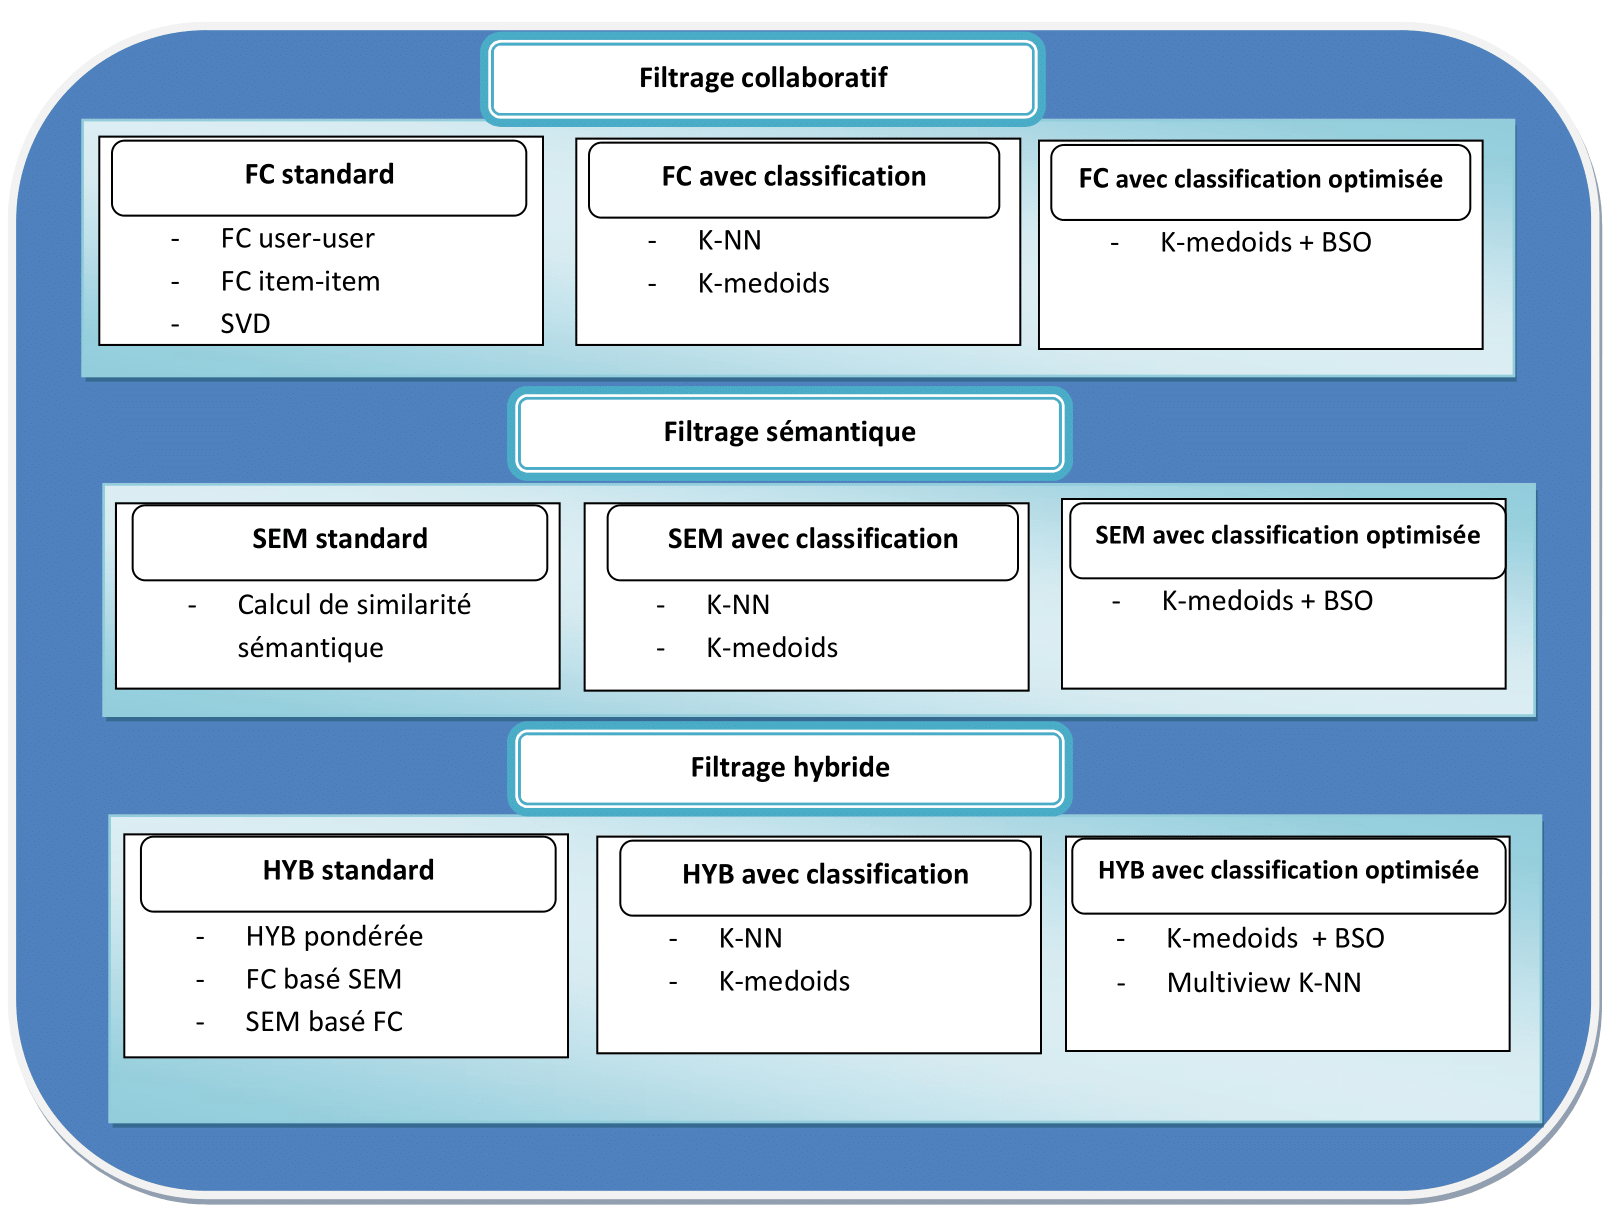
\includegraphics[width=\textwidth]{shema.png}
	\caption{Description générale de notre système de recommandation}
	\label{fig:shema}
\end{figure}

\section{Filtrage sans classification}
\subsection{Filtrage collaboratif}
Nous avons implémenté le filtrage collaboratif user-user,item-item, et une baseline qui est SVD.
\begin{enumerate}[nosep,label=\textbf{\arabic*)}]
	%%  \setcounter{enumi}{4}
	\item \textbf{Filtrage collaboratif standard}
\end{enumerate}\myparagraph{FC user-user}L'idée principale du FC user-user est d'utiliser la matrice d'usage pour déterminer les meilleurs voisins d'un utilisateur (parcours selon les lignes de la matrice), comme expliqué précédemment dans le chapitre 1. Le filtrage collaboratif passe par deux étapes, la première est le calcule de similarité et la détermination des voisins des utilisateurs, la deuxième consiste à effectuer la prédiction.

L'algorithme 1 ci-dessous décrit le FC basé user-user.

 \begin{algorithm}[H]
	\caption{FC}\label{FCUSERUSER}
	\hspace*{\algorithmicindent} \\
	\hspace*{\algorithmicindent} \textbf{Entrée:} Matrice{\_}usage, Seuil ;\\
	\hspace*{\algorithmicindent} \textbf{Sortie:} Ensemble de voisins de chaque utilisateur ;\\\\
	\hspace*{\algorithmicindent}\textbf{ Début:}
	\begin{itemize}
		
		\item []\textbf{Pour} Chaque \textit{utilisateur} de \textit{Matrice{\_}usage} \textbf{faire:} 
		   \begin{itemize}
		   	\item [] Calculer la distance entre cet utilisateur et tout les autres utilisateurs ;
		   	\item [] \textbf{Si:} distance  <= seuil \textbf{Alors} insérer cet utilisateur dans la table voisins du l'utilisateur en cours  \textbf{Fsi ;}
		   \end{itemize}
	   \item []\textbf{Fait ;} 
	
	\end{itemize}
	\hspace*{\algorithmicindent}\textbf{ Fin.}
\end{algorithm} 

\begin{itemize}
	\item \textbf{Seuil:} Nous déterminons le meilleur seuil pour le FC en évaluant les seuils générés à partir de la formule suivante:
	\begin{equation}
	Seuil=\frac{Min(matrice) + Max(matrice)}{10}
	\end{equation}
	Où Min() (respectivement Max()) est une fonction qui retourne la valeur minimum (respectivement maximum) de la matrice.
	À l'issue de l'application de cette formule nous obtenons dix seuils à tester, et nous choisirons celui qui nous donnera les meilleures prédictions. 
\end{itemize}

\begin{itemize}
	\item [-] \textbf{Complexité de l'algorithme}:
	\begin{itemize}
		\item [-] $n$: nombre d'utilisateurs.
		\item [-] Nous effectuons $n$ itérations pour calculer les voisins de chaque utilisateur.
	\end{itemize}
	\item [-] Donc la complexité de FC = $O(n)$
\end{itemize}


\myparagraph{FC item-item}
Comme pour le FC user-user, on détermine les voisins les plus proches des items avec la matrice d'usage mais cette fois-ci selon un parcours colonne par colonne.
\myparagraph {SVD (Singular Value decomposition)}
Dans le contexte des systèmes de recommandation, SVD est utilisée comme algorithme de filtrage collaboratif pour capturer la similarité entre les utilisateurs et les items en extrayant les caractéristiques cachées qu' utilisateur ou un item  possède et ainsi les faire correspondre selon leurs caractéristiques. 
Par exemple, pour les films, l'une des caractéristiques peut  être le genre auquel le film appartient comme comédie, horreur ou les deux en même temps et pour un utilisateur s'il a un caractère sérieux ou drôle ...ect, (voir figure ~\ref{fig:exemplefeatures}). 
Donc nous effectuons une décomposition en valeurs singulières pour extraire ces caractéristiques et avoir la meilleure décomposition de la matrice d'usage qui permet de prédire les ratings des items non encore évalués par les utilisateurs, souvent la métrique erreur racine moyenne (RMSE) est utilisée pour savoir si la décomposition et bonne ou pas(plus RMSE et bas mieux les performances et la prédiction est meilleure), on précise que nous prenons en compte que les ratings qu'on possède lors de la prédiction dans le calcul d'erreur.

SVD est effectué comme indiqué dans la figure \ref{fig:svd} ci-dessous.

\begin{figure}[H]
	\centering
	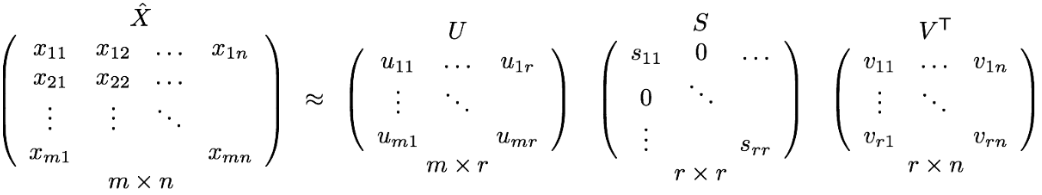
\includegraphics[width=\textwidth]{svd.png}
	\caption{Formule SVD}
	\label{fig:svd}
\end{figure}
Où:
\begin{itemize}
	\item  X: désigne la matrice d'utilité.
	\item  U: matrice singulière gauche, représentant la relation entre les utilisateurs et leurs caractéristiques.
	\item  S: matrice diagonale décrivant la force de chaque caractéristique.
	\item  V: matrice transposée singulière droite indiquant la similitude entre les items et leurs caractéristiques.
\end{itemize}



\begin{figure}[H]
	\centering
	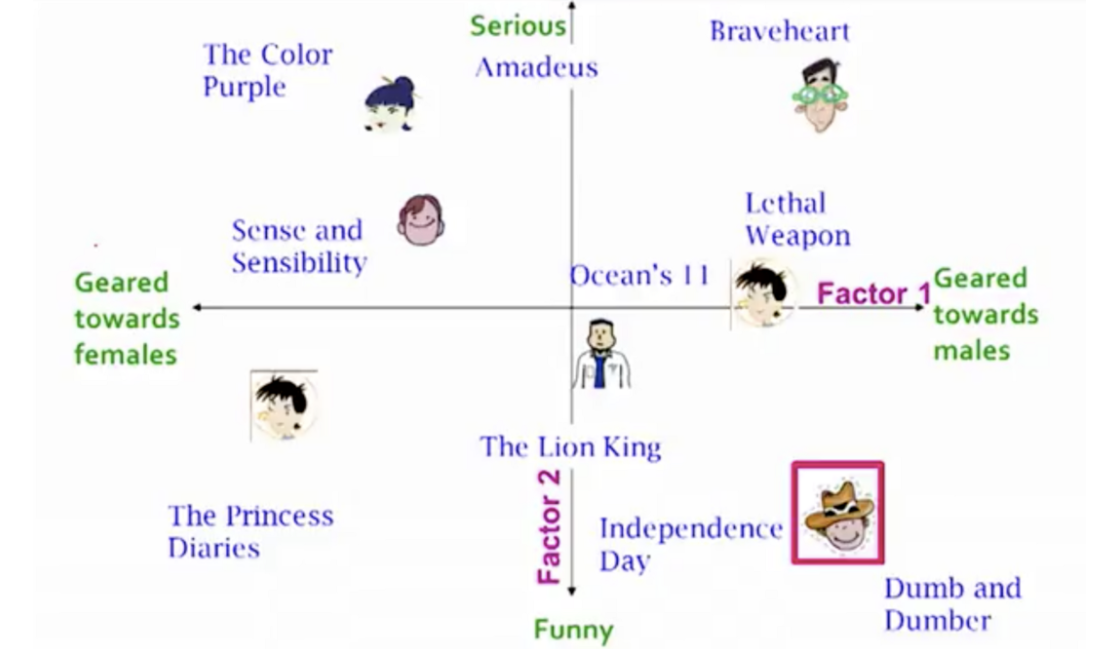
\includegraphics[width=\textwidth]{exemplefeatures.png}
	\caption{Exemple des caractéristiques d'un user \cite{ref31}}
	\label{fig:exemplefeatures}
\end{figure}

La figure \ref{fig:exemplesvd} ci-dessous montre un exemple de SVD

\begin{figure}[H]
	\centering
	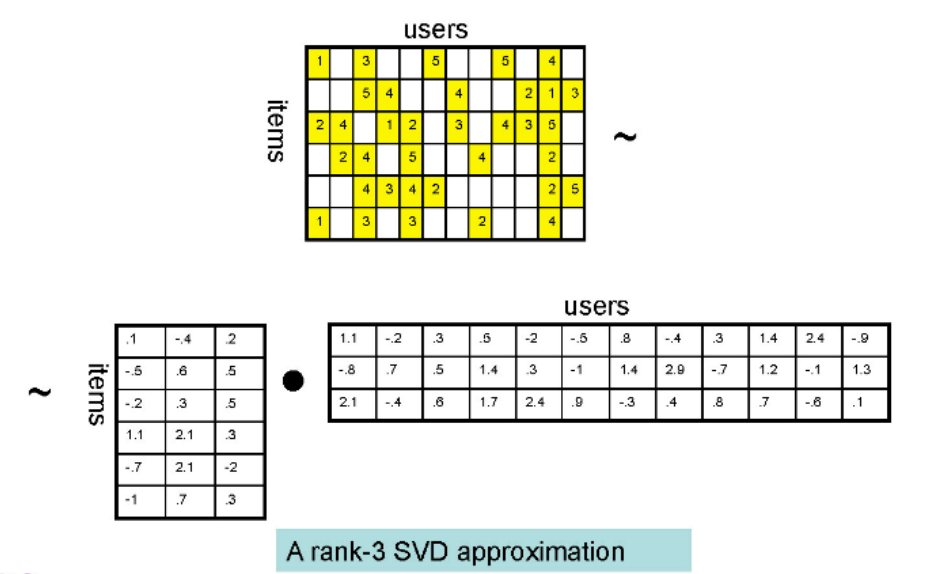
\includegraphics[width=\textwidth]{exempleofSVD.png}
	\caption{Exemple de Singular Value decomposition \cite{ref31}}
	\label{fig:exemplesvd}
\end{figure}
\myparagraph{Calcul de prédiction et distance pour le filtrage collaboratif}
Pour chaque algorithme FC cité précédemment, nous avons utilisé la formule de Pearson afin de calculer la distance entre les utilisateurs et les items, comme suit: 
\begin{itemize}
\item Calcul distance entre utilisateur:\\
Pour le calcul de distance entre deux utilisateurs u et v, la corrélation de Pearson est donnée par la formule suivante :
\begin{equation}\label{key21}
pearson(u,v)= 1 - \frac{\sum_{i \in I} (r_{u,i}-\bar{r}_{u}).(r_{v,i}-\bar{r}_{v})}{\sqrt{\sum_{i \in I} (r_{u,i}-\bar{r}_{u})^{2}.(r_{v,i}-\bar{r}_{v})^{2}}}
\end{equation}

où :
\begin{itemize}
	\item r $_{u,i}$ : est l'estimation de l'utilisateur u sur l’item i.
	\item r $_{v,i}$ : est l'estimation de l'utilisateur v sur l’item i.
	\item $\bar{r}_{u}$ : est la moyenne de toutes les notes de l'utilisateur u. 
	\item $\bar{r}_{v}$ : est la moyenne de toutes les notes de l'utilisateur v.
\end{itemize}

La distance est interprétée comme suit:

\begin{itemize}
	\item Si Pearson(u,v) = 0 alors les utilisateurs u et v sont parfaitement identiques.
	\item Si Pearson(u,v) = 1 alors les utilisateurs u et v ne sont pas corrélés. 
	\item Si 0 < Pearson(u,v) < 1  alors les utilisateurs u et v sont corrélés positivement (proches) et la distance représente le degrés de corrélation. 
	\item Si 1 < Pearson(u,v) < 2  alors les utilisateurs u et v sont corrélés négativement (loin) et la distance représente le degrés de corrélation. 
	\item Si Pearson(u,v) = 2 alors les utilisateurs u et v sont parfaitement opposés.
\end{itemize}

\item Calcul distance entre items:\\
Le calcul de distance entre deux items i et j : la corrélation de Pearson est donnée par la formule suivante :

\begin{equation}
pearson(i,j)= 1 - \frac{\sum_{u \in U} (r_{u,i}-\bar{r}_{i}).(r_{u,j}-\bar{r}_{j})}{\sqrt{\sum_{u \in U} (r_{u,i}-\bar{r}_{i})^{2}.\sum_{u \in U}(r_{u,i}-\bar{r}_{j})^{2}}}
\end{equation}

où :

\begin{itemize}
	\item r$_{u,i}$  : est l’évaluation de l’utilisateur u sur l’item i 
	\item r$_{u,j}$ : est l’évaluation de l’utilisateur u sur l’item j
	\item $\bar{r}_{i}$ : est la moyenne des évaluations de l’item i par les utilisateurs.
	\item $\bar{r}_{j}$ : : est la moyenne des évaluations de l’item j par les utilisateurs.
\end{itemize}
 
 
La distance est interprétée comme suit:
 
 \begin{itemize}
 	\item Si Pearson(i,j) = 0 alors les item i et j sont parfaitement identiques.
 	\item Si Pearson(i,j) = 1 alors les item i et j ne sont pas corrélés. 
 	\item Si 0 < Pearson(i,j) < 1  alors les item i et j  sont corrélés positivement (proches) et la distance représente le degrés de corrélation. 
 	\item Si 1 < Pearson(i,j) < 2  alors les item i et j sont corrélés négativement (loin) et la distance représente le degrés de corrélation. 
 	\item Si Pearson(i,j) = 2 alors les item i et j  sont parfaitement opposés.
 \end{itemize}


Pour la prédiction des valeurs des évaluations (ratings) des items non encore évalués, nous avons utilisé la formule de la somme pondérée:


\begin{equation}
pred(u_{i},i_{k})=\bar{r(u_{i})} + \frac{\sum_{u_{j} \in U_{i}} sim(u_{i},u_{j}).(r_{u_{j,ik}}-\bar{r(u_{j})})}{\sum_{u_{j} \in U_{i}} sim(u_{i},u_{j})}
\end{equation}

Où: 
\begin{itemize}
	\item sim(u$_{i}$,u$_{j}$) : est la mesure de similarité entre un utilisateur u$_{i}$ et son voisin u$_{j}$, tel que u$_{j}$ $\in$ U$_{i}$.
	\item $\bar{r}_{i}$ : est la moyenne des évaluations de l’item i par les utilisateurs.
	\item $\bar{r}_{j}$ : est la moyenne des évaluations de l’item j par les utilisateurs.
	
\end{itemize}
\end{itemize}
\subsection{Filtrage sémantique standard}
Ce type de filtrage utilise la notion sémantique pour déterminer les profils des utilisateurs qui sont similaires. Comme pour le filtrage collaboratif, le filtrage sémantique passe par deux étapes le calcule de similarité entre utilisateurs ensuite la prédication des ratings sur les items non évalués.

Pour déterminer si deux profils d'utilisateurs sont similaires du point de vue sémantique, nous nous intéressons aux items que les deux utilisateurs ont bien notés afin d'identifier les catégories qui sont susceptibles de les intéresser et donc par la suite leur recommander des items de catégories identiques ou similaires. 

C'est à partir de la catégorie d'un item que nous allons extraire l'information sémantique, pour cela nous disposons d'une matrice \textit{item-catégorie} qui contient pour chaque item donné la catégorie à laquelle il appartient.
Un item peut appartenir à plusieurs catégories en même temps, comme le montre la figure \ref{fig:cat} ci-dessous:

\begin{figure}[H]
	\centering
	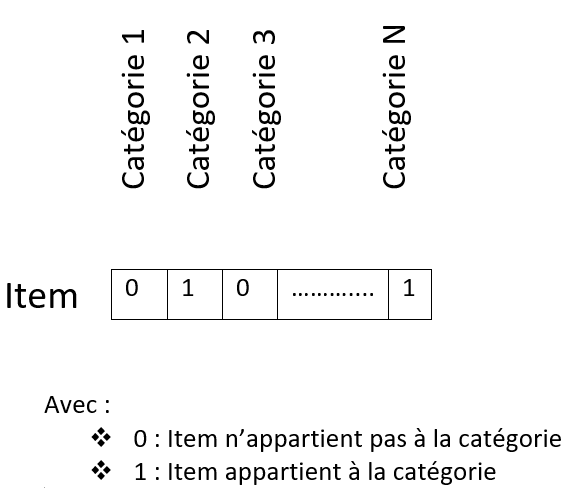
\includegraphics[width=0.60\textwidth]{movie-genre.PNG}
	\caption{Exemple d'une ligne de la matrice \textit{item-catégorie}}
	\label{fig:cat}
\end{figure}

Pour déterminer la similarité sémantique entres les items, nous devons calculer la distance entre ces derniers en se basant sur leurs représentation. Deux cas de figures se présentent à nous:
\begin{itemize}
	\item Les items ne sont pas représentés avec des ontologies: Pour chaque item de la matrice \textit{item-catégorie}, nous appliquons la distance de Jaccard  afin de déterminer les degrés de similarité entre les items et ainsi obtenir une matrice de distance \textit{item-item}. La distance de Jaccard est comprise entre $[0;1]$ et a la propriété d'être égale à 0 quand les items sont différents et 1 quand ils sont identiques et est calculée comme suit:
	
	\begin{equation}
	\displaystyle\text{J}(A,B) = 1 - \frac{|A\cap B|}{|A| + |B| -|A \cup B|} = 1 - \frac{\sum a_{i} * b_{i}}{\sum a_{i}^{2} + \sum b_{i}^{2} - \sum a_{i} * b_{i}}
	\end{equation}
	
	Où:
	\begin{itemize}
		\item $A$ et $B$: sont deux items,
		\item $a_{i}$, $b_{i}$: peuvent être soit 0 ou 1, ils indiquent l'appartenance ou non de l'item $A$ (respectivement $B$) à un une catégorie ${i}$ .
	\end{itemize}

\item Les items sont représentés avec des ontologies: Pour chaque item de la matrice \textit{item-catégorie}, nous appliquons la distance de Wu et Palmer  afin de déterminer les degrés de similarité entre les items et ainsi obtenir une matrice de distance \textit{item-item}. La distance de Wu et Palmer est comprise entre $[0;1]$. Si deux concepts sont identique la distance est égale à zéro et s'ils sont opposés elle est égale à un, et est calculée comme suit:

\begin{equation}
Dist_{WP}= 1 - \frac{ (2*N)}{(N_{1}+N_{2}+2*N)}
\end{equation}
Où:
\begin{itemize}
	\item $C1$ et $C2$: sont deux concepts.
	\item $N1$ et $N2$: la distance  séparant C1 et C2 du nœud racine.
	\item $N$: distance séparant l'ancêtre commun le plus proche de C1 et C2 du nœud racine.
\end{itemize}
\end{itemize}



\begin{figure}[H]
	\centering
	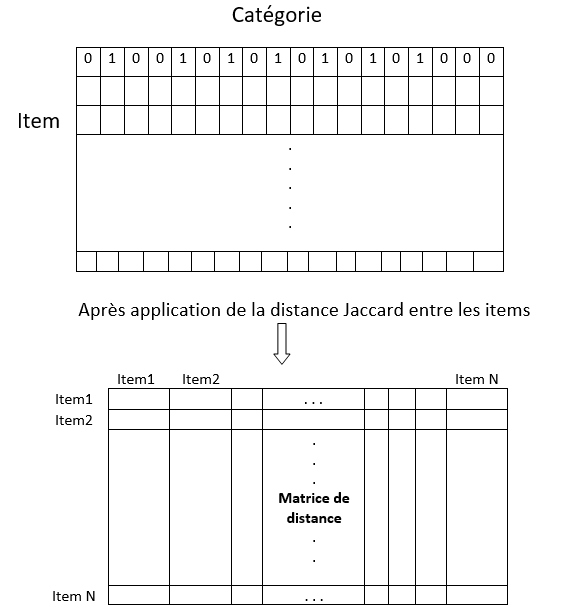
\includegraphics[width=\textwidth]{movie-movie-distance.PNG}
	\caption{Génération de la matrice de distance\textit{ item-item}}
\end{figure}

Après avoir obtenu la matrice distance\textit{ item-item} nous appliquons la formule de distance d'intérêt pour calculer la distance entre les utilisateurs de la matrice d'usage et ainsi obtenir la matrice de distance \textit{user-user} comme suit: 



\begin{equation}
d_{interest}(u,v) = \frac{\sum _{x \in X}n_{x} min_{y \in Y} d_{x,p} (x,y) + \sum_{y \in Y} n_{y} min_{x \in X} d_{w,p} (x,y)} {\sum _{x \in X} n_{x} + \sum _{y \in Y} n_{y}}
\end{equation}

Où: X (respectivement Y) sont les deux catégorie que u (respectivement v) a revu.



\begin{figure}[H]
	\centering
	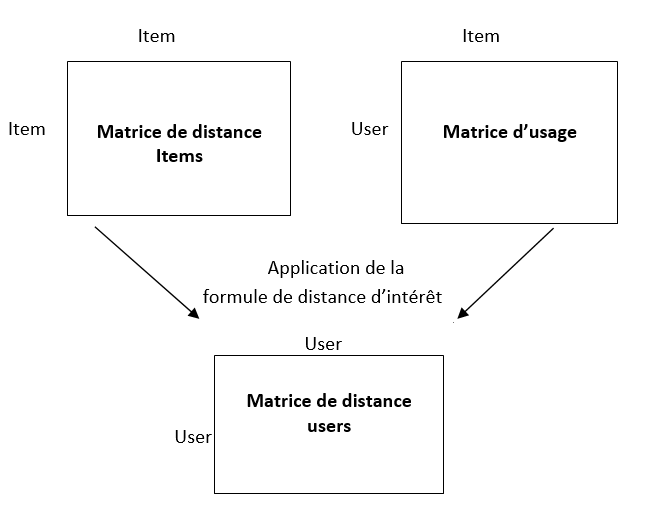
\includegraphics[width=0.8\textwidth]{user-user-interet.PNG}
	\caption{Génération de la matrice de distance \textit{user-user}}
\end{figure}

À partir de la matrice distancée \textit{user-user} nous pouvons déterminer à présent les voisins d'un utilisateur donné en appliquant l'algorithme suivant:

 \begin{algorithm}[H]
	\caption{Filtrage sémantique}
	\hspace*{\algorithmicindent} \\
	\hspace*{\algorithmicindent} \textbf{Entrée:} Matrice de distance user-user, Seuil;\\
	\hspace*{\algorithmicindent} \textbf{Sortie:} Ensemble de voisins de chaque utilisateur \\\\
	\hspace*{\algorithmicindent}\textbf{ Début:}
	\begin{itemize}
		
		\item []\textbf{Pour} Chaque \textit{utilisateur{\_}i} de \textit{matrice{\_}distance} \textbf{faire:} 
		\begin{itemize}
		\item []\textbf{Pour} Chaque \textit{distance{\_}j} de \textit{utilisateur{\_}i} \textbf{faire:} 
		\begin{itemize}
				\item [] /*récupérer l'indice de la colonne, qui représente l'indice du voisin en cours de traitement*/
			\item [] utilisateur{\_}j  $\leftarrow$ indice(distance{\_}j) 
			
			\item [] \textbf{Si:} \textit{distance{\_}j}  <= Seuil \textbf{Alors} insérer \textit{utilisateur{\_}j}  dans la table voisins du l'\textit{utilisateur{\_}i }\textbf{Fsi;}
		\end{itemize}
	
\item []  \textbf{Fait;}
\end{itemize}
\item []  \textbf{Fait;}
	\end{itemize}
	\hspace*{\algorithmicindent}\textbf{ Fin.}
\end{algorithm} 

\begin{itemize}
	\item \textbf{Seuil:} Le seuil est calculé de la même façon que pour le FC (voir seuil dans la partie FC).
\end{itemize}

\begin{itemize}
	\item [-] \textbf{Complexité de l'algorithme}:
	\begin{itemize}
		\item [-] $n$: nombre d'utilisateurs.
		\item [-] $n^2$: taille de la matrice de distance carré.
		\item [-] À chaque itération on fait un parcours de $n^2$ (taille de la matrice de distance).
	\end{itemize}
\item [-]  Donc la complexité du filtrage sémantique = $O(n^2)$
\end{itemize}

\myparagraph{Calcul de prédiction pour le filtrage sémantique}
Pour la prédiction des valeurs des ratings sur les items non encore évalués, nous avons utilisé la formule de la somme pondérée citée précédemment.

\subsection{Filtrage hybride}
Dans cette partie, nous allons détailler trois méthodes d'hybridation que nous avons implémentées entre les 2 types de filtrage déjà réalisés précédemment (sémantique, collaboratif), et qui sont:

\begin{itemize}
	\item Filtrage collaboratif hybride pondéré.
	\item Filtrage collaboratif basé sémantique.
	\item Filtrage sémantique basé collaboratif.
	
\end{itemize}

Pour chaque type d'hybridation conçu, les deux matrices de distance collaboratif (user-user, item-item) et sémantique jouent un rôle très important et sont calculées de la sorte:

\begin{itemize}
\item Matrice distance du filtrage collaboratif: 

Nous appliquons la formule Pearson pour calculer la distance d'un utilisateur avec le reste des utilisateurs de la  matrice d'usage et nous stockons les valeurs des distances dans une matrice comme le montre la figure \ref{fig:distuser} suivante: 

	\begin{figure}[H]
		\centering
		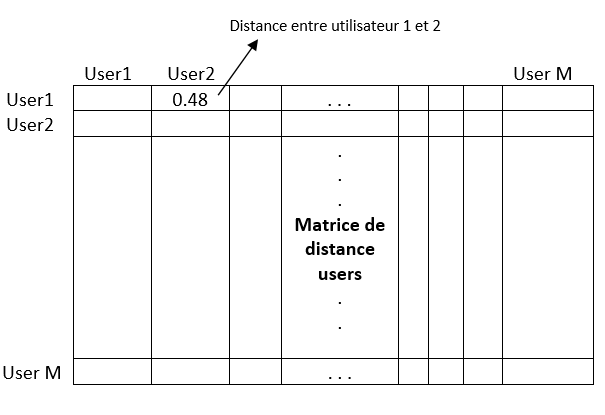
\includegraphics[width=0.80\textwidth]{matUserUSer.PNG}
		\caption{Matrice de distance user-user}
		\label{fig:distuser}
	\end{figure}

	\item  Matrice distance du filtrage sémantique: (voir explication dans la partie filtrage sémantique standard.)
\end{itemize}

\begin{enumerate}[nosep,label=\textbf{\arabic*)}]
	%%  \setcounter{enumi}{4}
	\item \textbf{Filtrage hybride pondéré}
\end{enumerate}\mbox{}\indent 
L'algorithme de filtrage hybride pondéré associe à chaque matrice de distance collaborative et sémantique respectivement un poids $\alpha$ et $\beta$ qui représentent les degrés d'importance de chaque type de recommandation (voir figure \ref{fig:alpha}) avec:
\begin{itemize}
	\item  $0.1 =< \alpha =< 0.9$
	\item  $\beta = 1 - Alpha$ 
	\item 	$\alpha + \beta = 1$
\end{itemize}

\begin{figure}[H]
	\centering
	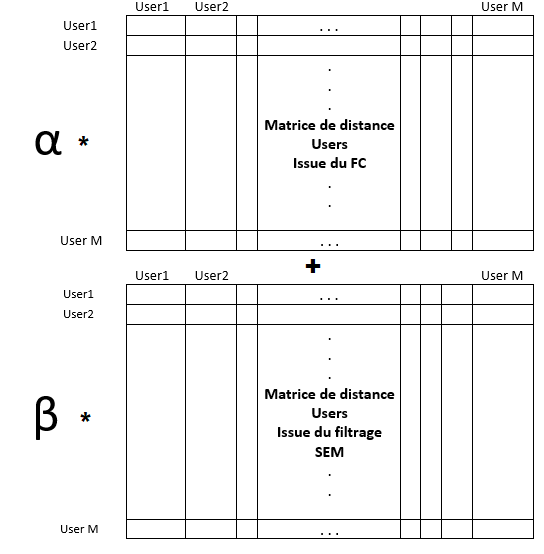
\includegraphics[width=0.9\textwidth]{hybpondere.PNG}
	\caption{Pondération des matrices de distances}
	\label{fig:alpha}
	
\end{figure}

Nous utilisons une boucle, dans laquelle nous augmentons la valeur de $\alpha$ de 0.1, et nous affectons à $\beta$ la valeur $1 - \alpha$, puis nous multiplions la matrice de distance du filtrage collaboratif par $\alpha$ et la matrice de distance du filtrage sémantique par $\beta$, nous évaluons par la suite les prédictions générées à partir de ces deux matrices, nous répétons ce processus jusqu'à ce que nous obtenons les meilleures valeurs possibles pour $\alpha$ et $\beta$ qui permettes d'accorder l'importance adéquate aux filtrages collaboratif et sémantique.

 \begin{algorithm}[H]
	\caption{Filtrage hybride pondéré}\label{HP}
	\hspace*{\algorithmicindent} \textbf{Entrée:}
	 \begin{itemize}
	\item [] Matrice{\_}distance{\_}FC: Matrice de distance du FC user-user , 
	\item [] Matrice{\_}distance{\_}SEM: Matrice de distance du filtrage sémantique user-user,
	\item [] Seuil{\_}Voisin: le seuil d'acceptation d'un voisin ;
	\end{itemize}
	\hspace*{\algorithmicindent} \textbf{Sortie:} 
	\begin{itemize}
	\item [] Ensemble de voisins pour chaque utilisateur selon meilleur poids Alpha ; 
	
	
	\end{itemize}
	
	\hspace*{\algorithmicindent}\textbf{ Début:}
	\begin{itemize}
		
		\item [] Alpha $\leftarrow$ 0.1 ;
		\item [] Beta $\leftarrow$ 1 - Alpha ;
		\item [] Best{\_}evaluation $\leftarrow$ Float(Inf) ;
		\item [] BestAlhpa $\leftarrow$ Float(Inf) ;
		\item []\textbf{Tant que } \textit{Beta >= 0.1}  \textbf{faire :} 
		\begin{itemize}
			
			\item [] AlphaMatrice $\leftarrow$  matrice{\_}distance{\_}FC * Alpha ;
			\item []Beta $\leftarrow$ 1 - Alpha ;
			\item [] BetaMatrice $\leftarrow$  matrice{\_}distance{\_}SEM * Beta ;
			\item  [] SommeMatrices $\leftarrow$  AphaMatrice +  BetaMatrice ;
			\item  [] Voisins{\_}users  $\leftarrow$ Voisin (SommeMatrices , Seuil{\_}Voisin) ;
			\item [] tableau{\_}prediciton $\leftarrow$  Prediction (usage{\_}matrice , Voisins{\_}users ) ;
			\item [] evaluation $\leftarrow$ Evaluation (tableau{\_}prediciton , reelles{\_}valeurs) ;
			\item [] \textbf{Si:} Best{\_}evaluation  >=  evaluation \textbf{Alors} 
			\begin{itemize}
				\item [] 	Swap (Best{\_}evaluation, evaluation) ;
				\item [] 	BestAlpha $\leftarrow$ valeurAlpha ;
			\end{itemize}	
				\item [] \textbf{Fsi ;}
				\item [] Alpha $\leftarrow$ Alpha - 0.1 ;
					
		\item [] \textbf{Fait ;} 
		\end{itemize}
		\item [] \textbf{Fait ;} 
	\end{itemize}
	\hspace*{\algorithmicindent}\textbf{ Fin.}
\end{algorithm} 

Où:
\begin{itemize}
	\item Voisins: Fonction qui calcule les voisins pour chaque utilisateur à partir d'un seuil et de la matrice de distance entre utilisateurs.
	\item Prediction: Fonction qui effectue les prédictions des items non évalués pour chaque utilisateur.
	\item Evaluation: Fonction qui calcule la qualité d'une prédiction effectuée. 
\end{itemize}

\begin{itemize}
	\item [-] \textbf{Complexité de l'algorithme}:
	\begin{itemize}
		\item [-] $n$: nombre d'utilisateurs.
		\item [-] $n^2$: taille de la matrice de distance carré.
		\item [-] Nous avons neuf itérations (de 0.1 jusqu'à 0.9).
		\item [-] À chaque itération on fait un parcours de $n^2$ (taille de la matrice de distance).
	\end{itemize}
	\item [-]  Donc la complexité du filtrage hybride pondéré = $O(9*n^2)$
\end{itemize}


\begin{enumerate}[nosep,label=\textbf{\arabic*)}]
	 \setcounter{enumi}{1}
	\item \textbf{Filtrage hybride sémantique basé collaboratif}
\end{enumerate}\mbox{}\indent Le filtrage sémantique standard décrit précédemment, utilise une matrice de distance entre les items qui est calculée avec la formule Jaccard, ici nous allons la remplacer avec la matrice de distance items issue du filtrage collaboratif (voir figure \ref{fig:semfc}) en utilisant la formule Pearson comme suit:
\begin{itemize}
	\item [-]Soit deux items i et j : la corrélation de Pearson est donnée par la formule suivante :
\end{itemize}
\begin{equation}
pearson(i,j)=\frac{\sum_{u \in U} (r_{u,i}-\bar{r}_{i}).(r_{u,j}-\bar{r}_{j})}{\sqrt{\sum_{u \in U} (r_{u,i}-\bar{r}_{i})^{2}.\sum_{u \in U}(r_{u,i}-\bar{r}_{j})^{2}}}
\end{equation}

Où:

\begin{itemize}
	\item r$_{u,i}$  : est l’évaluation de l’utilisateur u sur l’item i 
	\item r$_{u,j}$ : est l’évaluation de l’utilisateur u sur l’item j
	\item $\bar{r}_{i}$ : est la moyenne des évaluations de l’item i par les utilisateurs.
	\item $\bar{r}_{j}$ : est la moyenne des évaluations de l’item j par les utilisateurs.
\end{itemize}

\begin{figure}[H]
	\centering
	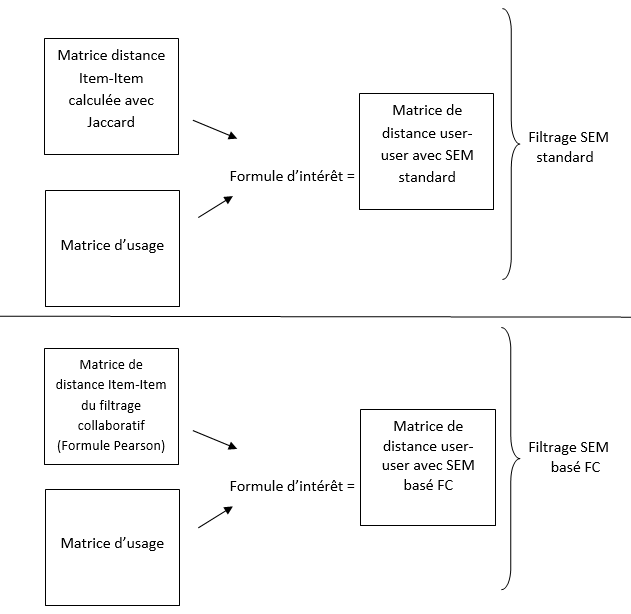
\includegraphics[width=\textwidth]{differance-entre-stand-sembasefc.PNG}
	\caption{Différence entre sémantique standard et sémantique basé collaboratif}
	\label{fig:semfc}
\end{figure}
\textbf{Remarque:} Après avoir passer en entrée la matrice de distance entre les items issue du FC, le même algorithme du filtrage sémantique est utilisé pour effectuer le filtrage sémantique basé collaboratif.
\myparagraph{Calcul de prédiction et distance pour le filtrage hybride sémantique basé collaboratif }
Pour la prédiction des valeurs des ratings sur les items non encore évalués, nous avons utilisé la formule de la somme pondérée citée précédemment.
Quant au calcule de distance entre utilisateurs elle s'effectue comme montré dans le filtrage sémantique en utilisant la même formule de calcul de distance d'intérêt (Formule 3.5). \\


\begin{enumerate}[nosep,label=\textbf{\arabic*)}]
	\setcounter{enumi}{2}
	\item \textbf{Filtrage hybride collaboratif basé sémantique}
\end{enumerate}\mbox{}\indent \iffalse  Dans le filtrage collaboratif, la matrice de distance est calculée avec la formule Pearson, qui donne une distance comprise entre [-1,1], si la distance est égale à 0 cela signifie qu'on ne sait pas si les deux utilisateurs sont corrélés ou pas et ça nous mène à un cas d'indétermination, donc pour y remédier on utilise la matrice de distance du filtrage sémantique dans le cas ou on trouve dans la matrice de distance du filtrage collaboratif \textit{user-user} des distances égalent à 0.
\fi Dans ce filtrage nous effectuons une séléction des voisins d'un utilisateur en utilisant les deux matrices de distance du FC et du filtrage sémantique.
Pour deux utilisateur A et B, B est considéré comme voisin de A ssi :\\
$\min( DFC(A,B) , DFSEM(A,B) ) <= seuil$
\\
Où:
\begin{itemize}
	\item DFC: distance ente utilisateur A et B selon le filtrage collaboratif.
	\item DFSEM: distance ente utilisateur A et B selon le filtrage sémantique.
	\item seuil: seuil d'acceptation d'un voisin pour un utilisateur donnée.
\end{itemize}

\begin{figure}[H]
	\centering
	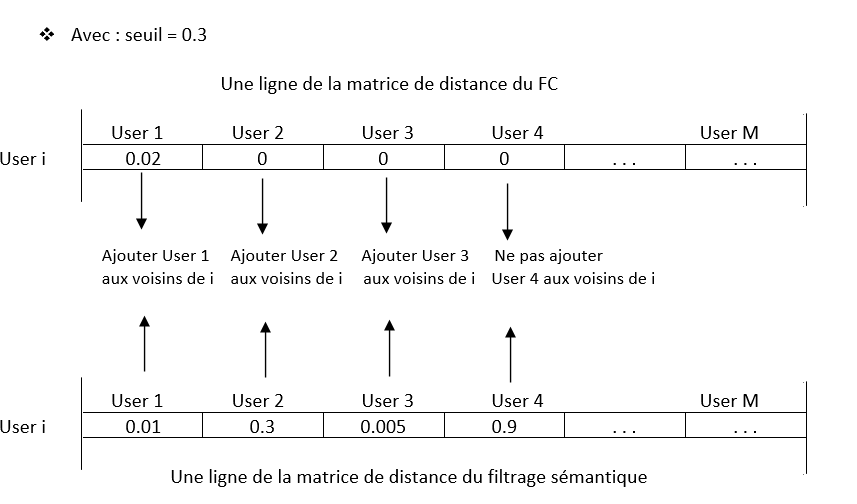
\includegraphics[width=\textwidth]{fcbasesem.PNG}
	\caption{Exemple de filtrage collaboratif-sémantique}
\end{figure}
\iffalse 
 \begin{algorithm}[H]
	\caption{Filtrage sémantique basé collaboratif}\label{sembasécol}
	\hspace*{\algorithmicindent} \\
	\hspace*{\algorithmicindent} \textbf{Entrée:} \begin{itemize}
		\item [] Matrice{\_}distance{\_}FC: Matrice de distance du FC user-user , 
		\item [] Matrice{\_}distance{\_}SEM: Matrice de distance du filtrage sémantique user-user;
		\item []  Seuil{\_}Voisin: le seuil d'acceptation d'un voisin ;
	\end{itemize}
	\hspace*{\algorithmicindent} \textbf{Sortie:} 
	\begin{itemize}
		\item [] Ensemble de voisins de chaque utilisateur
	\end{itemize}

	\hspace*{\algorithmicindent}\textbf{ Début:}
	
	\begin{itemize}
		\item [] \textbf{Pour} Chaque \textit{utilisateur{\_}i} de \textit{ Matrice{\_}distance{\_}FC} \textbf{faire:} 
	
		\begin{itemize}
		\item [] \textbf{Pour} Chaque \textit{distance{\_}j} de \textit{utilisateur{\_}i} \textbf{faire:} 
		\begin{itemize}
		\item [] /*récupérer l'indice de la colonne, qui représente l'indice du voisin en cours de traitement*/
		\item [] utilisateur{\_}j  $\leftarrow$ indice(distance{\_}j) 
		\item [] \textbf{Si:} distance{\_}j ==  0 \textbf{Alors} 
		\begin{itemize}
		\item [] distance{\_}j $\leftarrow$ Matrice{\_}distance{\_}SEM [ \textit{utilisateur{\_}i,utilisateur{\_}j }] \textbf{Fsi;}
		
		\end{itemize}
		\item [] \textbf{Si:} distance  <= Seuil \textbf{Alors} insérer utilisateur{\_}j  dans la table voisins du l'utilisateur{\_}i \textbf{Fsi;}
		\end{itemize}
	

		\end{itemize}
	\end{itemize}
		
	\hspace*{\algorithmicindent}\textbf{ Fin.}
\end{algorithm} 
\fi


\begin{algorithm}[H]
	\caption{Filtrage hybride collaboratif basé sémantique}
	\hspace*{\algorithmicindent} \\
	\hspace*{\algorithmicindent} \textbf{Entrée:} \begin{itemize}
		\item [] Matrice{\_}distance{\_}FC: Matrice de distance du FC user-user , 
		\item [] Matrice{\_}distance{\_}SEM: Matrice de distance du filtrage sémantique user-user;
		\item []  Seuil{\_}Voisin: le seuil d'acceptation d'un voisin ;
	\end{itemize}
	\hspace*{\algorithmicindent} \textbf{Sortie:} 
	\begin{itemize}
		\item [] Ensemble de voisins de chaque utilisateur ;
	\end{itemize}
	
	\hspace*{\algorithmicindent}\textbf{ Début:}


	
	\begin{itemize}
	\item []	Matrice{\_}distance $\leftarrow$ Min ( Matrice{\_}distance{\_}FC , Matrice{\_}distance{\_}SEM ) ;
		
		\item [] \textbf{Pour} Chaque \textit{utilisateur{\_}i} de \textit{ Matrice{\_}distance} \textbf{faire:}
				
		\begin{itemize}
			\item [] \textbf{Pour} Chaque \textit{distance{\_}j} de \textit{utilisateur{\_}i} \textbf{faire:} 
			\begin{itemize}
				\item [] /*récupérer l'indice de la colonne, qui représente l'indice du voisin en cours de traitement*/
				\item [] utilisateur{\_}j  $\leftarrow$ indice(distance{\_}j) 

				\item [] \textbf{Si:} distance{\_}j  <= Seuil \textbf{Alors} insérer utilisateur{\_}j  dans la table voisins du l'utilisateur{\_}i \textbf{Fsi;}
			\end{itemize}
			
			\item []  \textbf{Fait;}
		\end{itemize}
	\item []  \textbf{Fait;}
	\item [] \textbf{ Fin.}
	\end{itemize}
	

\end{algorithm} 

Où:
\begin{itemize}
	\item Min(): Fonction qui prend minimum des distances entre deux matrices et les stocke dans une nouvelle matrice.
\end{itemize}

\begin{itemize}
	\item [-] \textbf{Complexité de l'algorithme}:
	\begin{itemize}
		\item [-] $n$: nombre d'utilisateurs.
		\item [-] $n^2$: taille de la matrice de distance carré.
		\item [-] À chaque itération on fait un parcours de $n^2$ (taille de la matrice de distance).
	\end{itemize}
	\item [-]  Donc la complexité du filtrage collaboratif basé sémantique = $O(n^2)$
\end{itemize}


\section{Filtrage avec classification}
Dans cette partie, nous allons expliquer l'amélioration apportée aux différents filtrages conçus jusqu'à présent en leurs ajoutant une technique de classification, on précise que la matrice de distance que nous allons utiliser pour classifier les utilisateurs est le résultat d'une des variantes du FC, notre choix sera basé sur les tests effectués afin de prendre la meilleure variante, donc nous aurons à choisir entre FC item-item, FC user-user ou SVD. Concernant le FSem nous avons conçu une seule variante par conséquent il n'y aura pas de choix à faire. Enfin, pour le filtrage hybride nous incorporons la classification dans les trois méthodes réalisées (filtrage hybride pondéré, collaboratif basé sémantique et sémantique basé collaboratif.(voir figure \ref{fig:selec})

\begin{figure}[H]
	\centering
	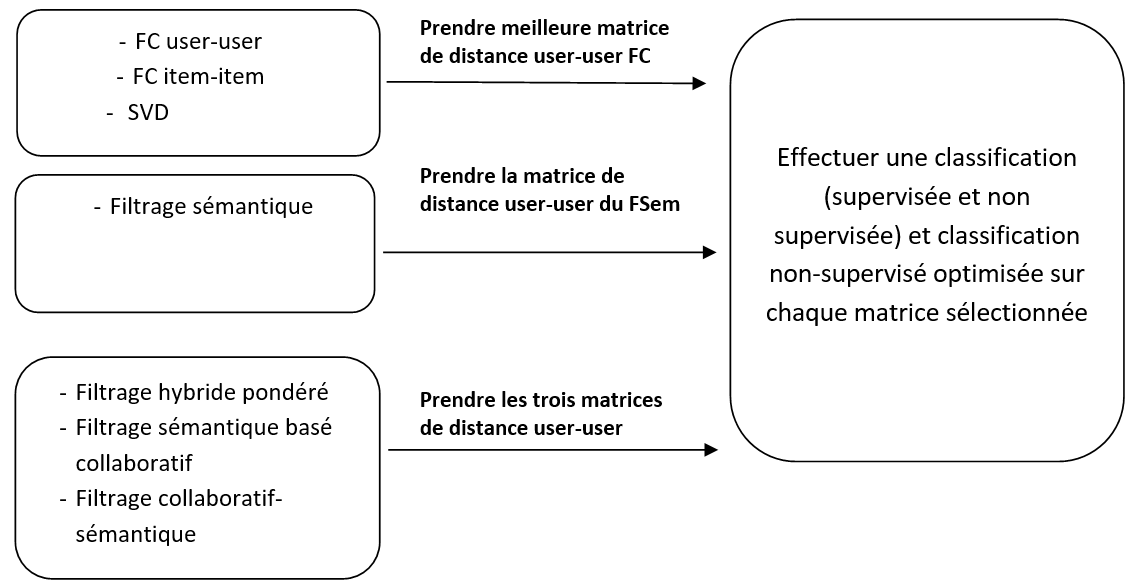
\includegraphics[width=1.1\textwidth]{selectionbestmat.PNG}
	\caption{Sélection des matrices de distance \textit{user-user} pour l'application de la classification}
	\label{fig:selec}
\end{figure}

\subsection{Filtrage avec classification supervisée}
\begin{enumerate}[nosep,label=\textbf{\arabic*)}]
	%%  \setcounter{enumi}{4}
	\item \textbf{K-NN}
\end{enumerate}\mbox{}\indent Comme motionné dans le chapitre 2, K-NN est un algorithme d'apprentissage automatique. Dans notre cas nous l'avons utilisé pour effectuer les prédictions d'un utilisateur donné, en se basant sur ses voisins les plus proches. Nous avons besoin donc des distances entre utilisateurs sous forme de matrice de distance \textit{user-user} issue d'un des type de filtrage et \textit{K} qui est le nombre de voisins à considérer.

Par exemple pour effectuer un filtrage sémantique basé K-NN, il suffit d'envoyer à l'algorithme ci-dessous la matrice de distance \textit{user-user} issue du filtrage sémantique.
Il en est de même pour effectuer:
\begin{itemize}
	\item Filtrage collaboratif basé K-NN.
	\item Filtrage hybride pondéré basé K-NN.
	\item Filtrage collaboratif basé sémantique avec classification K-NN.
	\item Filtrage sémantique basé collaboratif avec  classification K-NN.
\end{itemize}

\begin{algorithm}[H]
	\caption{Filtrage avec classification supervisée (K-NN)}
	\hspace*{\algorithmicindent} \\
	\hspace*{\algorithmicindent} \textbf{Entrée:} \begin{itemize}
		\item [] Matrice{\_}distance{\_}user-user: Matrice de distance issue d'un des types de filtrage , 
		\item []  K: le nombre de voisins à considérer dans les prédictions;
	\end{itemize}
	\hspace*{\algorithmicindent} \textbf{Sortie:} 
	\begin{itemize}
		\item [] Ensemble de K voisins de chaque utilisateur ;
	\end{itemize}
	
	\hspace*{\algorithmicindent}\textbf{ Début:}
	
	\begin{itemize}
		\item [] Voisins[ ] ;/*Liste de listes qui contient les voisins des utilisateurs*/
		\item [] \textbf{Pour} Chaque \textit{utilisateur{\_}i} de \textit{ Matrice{\_}distance{\_}user-user} \textbf{faire:} 
			
			\begin{itemize}
				\item [] /*trier selon l'ordre croissant les distances entre l'utilisateur i et le reste des utilisateur du dataset contenu dans la ligne utilisateur{\_}i */
				\item []	sortedListe $\leftarrow$ Sort(utilisateur{\_}i) ;
			\item []	/*Récupérer les indices des K plus proches voisins de l'utilisateur{\_}i/
				\item [] Voisins[utilisateur{\_}i] $\leftarrow$ Min{\_}K{\_}distance(K,indice(soretedListe)) ;
				
			\end{itemize}
		\end{itemize}
		
		\hspace*{\algorithmicindent}\textbf{ Fin.}
	\end{algorithm} 

\begin{itemize}
	\item [-] \textbf{Complexité de l'algorithme}:
	\begin{itemize}
		\item [-] $n$: nombre d'utilisateurs.
		\item [-] CAAT: complexité approximative de l'algorithme de trie.
		\item [-] À chaque itération on fait un parcours de $n$ (taille de la matrice de distance).
	\end{itemize}
	\item [-]  Donc la complexité du filtrage avec classification supervisée = $O(n*CAAT)$
\end{itemize}
	
\mbox{}
\begin{enumerate}[nosep,label=\textbf{\arabic*)}]
	  \setcounter{enumi}{1}
	\item \textbf{Hybridation mutivues, collaborative et sémantique, basé sur K-NN}
\end{enumerate}\mbox{}\indent Cette approche est inspirée du travail des chercheurs Guibing Guo et al. \cite{ref30}, dans lequel ils effectuent un clustering des utilisateurs en appliquant deux fois consécutives k-medoids (une fois selon la vue similarité et la deuxième fois selon la vue de confiance entre utilisateurs) et par la suite combiner le résultat des deux vues.
Nous avons étudié leur travail et put aboutir à l'idée d'utiliser l'algorithme K-NN selon nos deux vues sémantique et collaboratif.
Le choix de l'algorithme K-NN semble adéquat aux données et informations dont on dispose, de plus c'est un algorithme simple et très utilisé dans la recommandation.

L'idée générale de notre approche est d'effectuer une classification K-NN sur la matrice de distance \textit{user-user} du FC et de prendre K utilisateurs ce qui nous donne une classification selon une première vue, par la suite refaire la même chose sur la matrice de distance \textit{user-user} du filtrage sémantique  pour avoir la deuxième vue, enfin combiner les deux classifications en exécutant K-NN une autre fois sur les K utilisateurs issues de la première classification et de la deuxième (voir figure \ref{fig:knn}).


\begin{figure}[H]
	\centering
	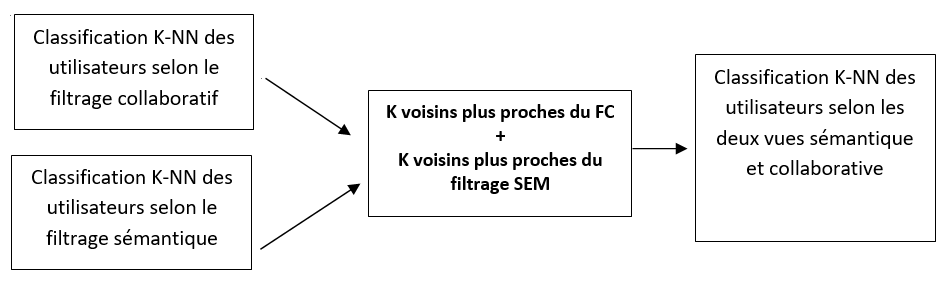
\includegraphics[width=\textwidth]{multiviewknn.PNG}
	\caption{Schéma du filtrage multiview K-NN}
	\label{fig:knn}
\end{figure} 

\begin{algorithm}[H]
	\caption{Filtrage avec multiview (K-NN) Partie 1}
	\hspace*{\algorithmicindent} \\
	\hspace*{\algorithmicindent} \textbf{Entrée:} \begin{itemize}
		\item [] Matrice{\_}distance{\_}user-user{\_}FC: Matrice de distance issue d'un du filtrage collaboratif,
		\item [] Matrice{\_}distance{\_}user-user{\_}SEM: Matrice de distance issue d'un du filtrage sémantique,
		\item []  K: le nombre de voisins à considérer dans les prédictions;
	\end{itemize}
	\hspace*{\algorithmicindent} \textbf{Sortie:} 
	\begin{itemize}
		\item [] Ensemble de K voisins de chaque utilisateur selon les deux vues ;
	\end{itemize}
	
	\hspace*{\algorithmicindent}\textbf{ Début:}
	\hspace*{\algorithmicindent}\\Voisins[ ]{\_}CF ;/*Liste de listes qui contient les voisins des utilisateurs selon filtrage collaboratif*/
	\hspace*{\algorithmicindent}\\ Voisins[ ]{\_}SEM ;/*Liste de listes qui contient les voisins des utilisateurs selon filtrage sémantique*/
\hspace*{\algorithmicindent}\\\textbf{Pour} Chaque \textit{utilisateur{\_}i} de \textit{ Matrice{\_}distance{\_}user-user{\_}CF} \textbf{faire:} 
		
		\begin{itemize}
			\item [] /*trier selon l'ordre croissant les distances entre l'utilisateur i et le reste des utilisateur du dataset contenu dans la ligne utilisateur{\_}i */
			\item []	sortedListe $\leftarrow$ Sort(utilisateur{\_}i) ;
			\item []	/*Récupérer les indices des K plus proches voisins de l'utilisateur{\_}i/
			\item [] Voisins[utilisateur{\_}i]{\_}CF$\leftarrow$ Min{\_}K{\_}distance(K,indice(soretedListe)) ;
			
		\end{itemize}
	
	
	 \textbf{Pour} Chaque \textit{utilisateur{\_}i} de \textit{ Matrice{\_}distance{\_}user-user{\_}SEM} \textbf{faire:} 
	
	\begin{itemize}
		\item [] /*trier selon l'ordre croissant les distances entre l'utilisateur i et le reste des utilisateur du dataset contenu dans la ligne utilisateur{\_}i */
		\item []	sortedListe $\leftarrow$ Sort(utilisateur{\_}i) ;
		\item []	/*Récupérer les indices des K plus proches voisins de l'utilisateur{\_}i/
		\item [] Voisins[utilisateur{\_}i]{\_}SEM$\leftarrow$ Min{\_}K{\_}distance(K,indice(soretedListe)) ;
		
	\end{itemize}

\end{algorithm} 

\setcounter{algorithm}{5}
\begin{algorithm}[H]
\caption{Filtrage avec multiview (K-NN) Partie 2}
/*Fusionner les deux vues*/
\hspace*{\algorithmicindent} \\Voisins[ ]$\leftarrow$ Voisins[utilisateur{\_}i]{\_}SEM + Voisins[utilisateur{\_}i]{\_}CF ;

\textbf{Pour} Chaque \textit{utilisateur{\_}i} de \textit{ Voisins[ ]} \textbf{faire:} 

\begin{itemize}
	\item [] /*trier selon l'ordre croissant les distances entre l'utilisateur i et le reste des utilisateur du dataset contenu dans la ligne utilisateur{\_}i */
	\item []	sortedListe $\leftarrow$ Sort(utilisateur{\_}i) ;
	\item []	/*Récupérer les indices des K plus proches voisins de l'utilisateur{\_}i/
	\item [] Voisins[utilisateur{\_}i]{\_}Multiview $\leftarrow$ Min{\_}K{\_}distance(K,indice(soretedListe)) ;
	
\end{itemize}

\textbf{ Fin.}
\end{algorithm} 
\begin{itemize}
	\item [-] \textbf{Complexité de l'algorithme}:
	\begin{itemize}
		\item [-] $n$: nombre d'utilisateurs.
		\item [-] CAAT: complexité approximative de l'algorithme de trie.
		\item [-] Nous effectuons trois fois l'algorithme K-NN.
		\item [-] À chaque itération on fait un parcours de $n$ (taille de la matrice de distance).
	\end{itemize}
	\item [-]  Donc la complexité du filtrage avec classification supervisée = $O(3*n*CAAT)$
\end{itemize}


\subsection{Filtrage avec classification non supervisée}
\begin{enumerate}[nosep,label=\textbf{\arabic*)}]
	%%\setcounter{enumi}{1}
	\item \textbf{Filtrage basé sur K-medoids}
\end{enumerate}\mbox{}\indent Le principe est d'appliquer l'algorithme K-medoids sur l'ensemble des utilisateurs de manière à construire des clusters qui contiennent des utilisateurs possédant des intérêts similaires, le choix des utilisateurs qui seront considérés comme medoids de départ s'effectue de façon aléatoire.
Les distances entre les utilisateurs sont stockées dans les matrice distance \textit{user-user} issue d'un des type de filtrage.

Par exemple pour effectuer un filtrage sémantique basé K-medoids, il suffit d'envoyer à l'algorithme ci-dessous la matrice de distance \textit{user-user} issue du filtrage sémantique.
Il en est de même pour effectuer:
\begin{itemize}
	\item Filtrage collaboratif basé K-medoids.
	\item Filtrage hybride pondéré basé K-medoids.
	\item Filtrage collaboratif basé sémantique avec clustering K-medoids.
	\item Filtrage sémantique basé collaboratif avec clustering K-medoids.
\end{itemize}


\begin{algorithm}[H]
	\caption{Filtrage avec classification non supervisé  (K-medoids)}
	\hspace*{\algorithmicindent} \\
	\hspace*{\algorithmicindent} \textbf{Entrée:}
		\begin{itemize}
		\item [] Matrice{\_}distance{\_}user-user: Matrice qui contient les distances entre utilisateur issue d'un des types de filtrage , 
		\item [] K: Le nombre de cluster à former ;
		\end{itemize}
		\hspace*{\algorithmicindent} \textbf{Sortie:} 
	\begin{itemize}
		\item [] Clustering des utilisateurs en K cluster ;
	\end{itemize}
	\hspace*{\algorithmicindent}\textbf{ Début:}	
		
		\begin{itemize}
		\item  [] Medoids $\leftarrow$ Choisir les K centres  des clusters : Désigné aléatoirement K indices de la matrice de distances représentant les indices de K utilisateurs ;
		\item [] calculer le cout initial;	

		\item [] \textbf{Pour} Chaque \textit{M-user } de \textit{Medoids} \textbf{faire:}
		\begin{itemize}
			\item [] \textbf{Pour} Chaque \textit{N-user}  de \textit{non-Medoids} \textbf{faire:}
			\begin{itemize}
				\item [] Swap(M,O) ;
				\item [] Distribution(Matrice{\_}distance{\_}user-user, Medoids) ;
				\item [] calculerCout( );
				\item []  \textbf{Si:} le cout de cette itération est supérieure au cout de l'itération précédente \textbf{alors} Undo(M-user,N-user) ; \textbf{Fsi;}	
				\item []  \textbf{Si:} Aucune changement alors arrêter l'algorithme \textbf{Fsi;}			
				
			\end{itemize}
			\item []\textbf{Fait;}
		\end{itemize}
		\item []\textbf{Fait;}
		\end{itemize}

	\hspace*{\algorithmicindent}\textbf{ Fin.}	
\end{algorithm}

Où: 
\begin{itemize}
	\item [-] Swap() : Remplace le medoid M-user par N-user
	\item [-] Undo() : Annule le swap de M-user par N-user
	\item [-] Distribution() : Assigne les utilisateurs au plus proche cluster en utilisant la matrice de distance et les medoids 
	\item [-] Cout() : Fonction objective qui est destinée à être minimisée
\end{itemize}

\begin{equation}
Cout=\min\sum_{c \in C}\sum_{u,v \in c}d(u,v)
\end{equation}

Avec : C l'ensemble des clusters résultant de l'lagorithme k-medoids, u et v deux utilisateurs, v appartient au cluster et u son medoids.

\begin{itemize}
	\item [-] \textbf{Complexité de l'algorithme}:
	\begin{itemize}
		\item [-] $n$: nombre d'utilisateurs.
		\item [-] $k$: nombre de clusters à former.
		\item [-] Nous devons trouver la distance entre chacun des $(n-k)$ points de données k fois pour placer les points de données dans le groupe le plus proche.
		\item [-] Après cela, nous devons remplacer chacun des medoids précédemment supposés par chaque non-medoid et recalculer la distance entre les objets $(n-k)$.
	\end{itemize}
	\item [-]  Donc la complexité du filtrage avec classification non supervisée = $O(k(n-k)^2)$
\end{itemize}


\subsection{Filtrage avec classification non supervisée optimisée}
Comme nous l'avons vu dans le chapitre précédent l'optimisation par colonie d'abeilles manipule un ensemble d'abeilles où chaque abeille correspond à une solution faisable d'un problème donné.
Nous avons décider d'exploiter le mieux possible BSO dans le but d'optimiser le clustering effectué par K-medoids, et ainsi améliorer la qualité des prédictions.

K-medoids commence initialement par des medoids qui sont sélectionnés aléatoirement, en utilisant BSO nous tentons de trouver les meilleurs medoids de départ qui permettent de faire le meilleur partitionnement possible des utilisateurs, et de ne pas effectuer une sélection aléatoire des medoids car nous avons peu de chance de tomber sur de bons medoids.

Cette classification non supervisée optimisée est appliquée pour les différents types de filtrage conçu (FC, FSem et Filtrage hybride) car 
nous faisons appelle à l'algorithme BSO qui lui fait appelle à l'algorithme K-medoids, ce dernier comme vu précédemment (voir Filtrage basé sur K-medoids) à en entrée une matrice de distance issue de l'un des types de filtrages implémentés.\\

\begin{enumerate}[nosep,label=\textbf{\arabic*)}]
	%%\setcounter{enumi}{1}
	\item \textbf{Codification et initialisation de la solution}
\end{enumerate}\mbox{}\indent Afin d'exploiter le mieux possible la métaheuristique et prouver son efficacité il est nécessaire de faire une codification adéquate qui permet de modéliser le problème.
Dans notre cas, chaque partitionnement des users effectué par k-medoids représente une solution, donc chaque abeille correspond à un partitionnement faisable.

La solution est représentée par un vecteur de taille égale au nombre d'utilisateurs à classifier dans un dataset, les indices du vecteur représentent les identificateurs des utilisateurs et chaque case du vecteur peut contenir un 0 ou 1 qui signifient respectivement:
\begin{itemize}
	\item le i ème utilisateur du vecteur solution n'est pas medoid.
	\item le i ème  utilisateur de vecteur solution est medoid.
\end{itemize}

On démarre l'algorithme avec une solution initiale qui est soit aléatoire en remplissant un vecteur de taille N (N = nombre d'utilisateurs) avec 0 et 1, ou une solution qui est le résultat d'un vecteur construit à partir des clusters sorties de l'algorithme K-medoids qui représente un partitionnement des utilisateurs en K clusters.\\

\begin{enumerate}[nosep,label=\textbf{\arabic*)}]
	\setcounter{enumi}{1}
	\item \textbf{Pseudo code de l'algorithme BSO adapté au probléme de recommandation}
\end{enumerate}\mbox{}\indent Le pseudo-code suivant explique le principe de l'algorithme BSO adapté à notre problème. À noter qu'à chaque ajout d'une solution référence on doit vérifier qu'elle n'est pas déjà dans la liste taboue.  


\begin{algorithm}[H]
	\caption{Recommandation avec K-medoids optimisée (BSO) partie 1}
	\hspace*{\algorithmicindent} \textbf{Entrée:}
	\begin{itemize}
		\item [] Matrice{\_}distance{\_}user-user: Matrice qui contient les distances entre utilisateur issue d'un des types de filtrage , 
		\item [] K: Le nombre de cluster à former,
		\item [] nbrIteration, flip, local{\_}max{\_}iter ;
	\end{itemize}
	\hspace*{\algorithmicindent} \textbf{Sortie:} 
	\begin{itemize}
		\item [] Vecteur de solution optimisé par BSO;
	\end{itemize}
	\hspace*{\algorithmicindent}\textbf{ Début:}	
	
\hspace*{\algorithmicindent}	\\/*Generation aléatoire de Sref (vecteur à valeurs entre 0 et 1)*/
 \hspace*{\algorithmicindent}	\\/*ou appeler K-medoids pour générer une solution avec K-1 medoids*/  
	\hspace*{\algorithmicindent} \\(Sref $\leftarrow$ Random-sol() || Sref $\leftarrow$ K-medoids(K-1, Matrice{\_}distance{\_}user-user)) ;
	\hspace*{\algorithmicindent}\\ /*Evaluer la solution Sref et la définir comme meilleure évaluation pour le moment*/  
		\hspace*{\algorithmicindent}\\  Best{\_}eval = Eval(sref);
	\hspace*{\algorithmicindent}\\  \textbf{Pour} \textit{cpt} de \textit{nbrIteration} \textbf{faire:}
			\begin{itemize}
				\item [] /*Ajouter la solution de référence à tabou liste*/
				\item [] taboo-list.append(Sref);	
				\item [] /*Generer les solutions a partir de Sref avec paramètre flip*/
				\item [] areas $\leftarrow$ search-area(Sref,flip);
				\item [] /* Début de la boucle de locale*/
				\item  [] \textbf{Pour} Chaque \textit{area} de \textit{areas} \textbf{faire:}
				\begin{itemize}
					\item [] /*Recherche local dans le voisinage de la solution courante*/
					\item []   current{\_}eval, solution = bee-local-search(area, local{\_}max{\_}iter);
					\item [] \textbf{Si:}  Best{\_}eval < min{\_}eval \textbf{alors:}
					\begin{itemize}
						\item []  Best{\_}eval $\leftarrow$ min{\_}eval;
						\item [] Sref $\leftarrow$  solution ;
					\end{itemize}
					
					\item []  \textbf{Fsi;}		
				\end{itemize}
				\item []  \textbf{fait;}	
			\end{itemize}
		
\end{algorithm}	
\setcounter{algorithm}{7}
\begin{algorithm}[H]
\caption{Recommandation avec K-medoids optimisée (BSO) partie 2}	
\hspace*{\algorithmicindent}\\ /*A la sortie de la boucle de la recherche locale, nous aurons une solution \textit{Sref} qui donne la meilleure évaluation, si \textit{nbriterations} n'est pas atteint alors nous générons des solutions à partir de \textit{Sref} et nous re-effectuant une recherche locale, sinon on sort avec la meilleure solution qui est \textit{Sref}*/
\hspace*{\algorithmicindent}\\  \textbf{fait;}

\hspace*{\algorithmicindent}\textbf{Fin.}
\end{algorithm}

Où:
\begin{itemize}
	\item search-area(): génère un espace de recherche à partir de Sref.
	\item bee-local-search(): permet d'effectuer une recherche local à partir d'une solution donnée,
	\item Eval(): évalue la qualité d'une solution donnée.
\end{itemize}
\begin{itemize}
	\item [-] \textbf{Complexité de l'algorithme}: Soient les variables suivantes :
	\begin{itemize}
	\item	GMI: nombre global de max itération.
	\item	LMI: nombre local de max itération.
	\item	EACK: estimation approximative de la complexité de kmedoids.
	\item	flip: paramètre empirique qui détermine le nombre de search areas.
	\end{itemize}
	\item [-] Donc complexité de BSO = $O(GMI*flip*LMI*EACK)$
\end{itemize}

\begin{enumerate}[nosep,label=\textbf{\arabic*)}]
	\setcounter{enumi}{2}
	\item \textbf{Flip}
\end{enumerate}\mbox{}\indent Détermine le nombre d'espace de recherche à générer à partir de \textit{Sref}, une valeur trop grande donnée au \textit{flip} implique dans notre cas la génération de plusieurs espaces de recherche et donc une bonne diversification et en même temps une intensification de la recherche, car il existerait des solutions qui seront proches dues au fait de la rotation à gauche qu'on effectue pour générer \textit{flip} solutions à partir de \textit{Sref}, tant dit qu'un petit \textit{flip} n'impliquerait qu'une intensification de la recherche dans un voisinage proche (voir figure \ref{fig:bsosearch}).\\


\begin{enumerate}[nosep,label=\textbf{\arabic*)}]
	\setcounter{enumi}{3}
	\item \textbf{L'espace de recherche}
\end{enumerate}\mbox{}\indent
\textbf{Exemple:}
Si on suppose que \textit{nbr{\_}medoid} = 4 et \textit{nbr-user} = 7, au départ nous générons un vecteur \textit{Sref} qui représente une solution de taille égale à 7 avec 3 medoids donc trois 1 seront présents dans le vecteur \textit{Sref}, par la suite nous générons un espace de recherche initiale à partir de \textit{Sref}  en prenant \textit{flip = nbr{\_}medoid / flip}, donc nous aurons \textit{flip} solutions générée à partir de \textit{Sref} en effectuant une rotation à gauche \textit{flip} fois, enfin nous envoyons à chaque abeille ( \textit{flip} abeille ) une solution pour qu'elle commence une recherche locale afin de trouver le 4ème medoids qui donne les meilleures évaluations possibles (voir figure \ref{fig:bsosearch}).

 \begin{figure}[H]
	\centering
	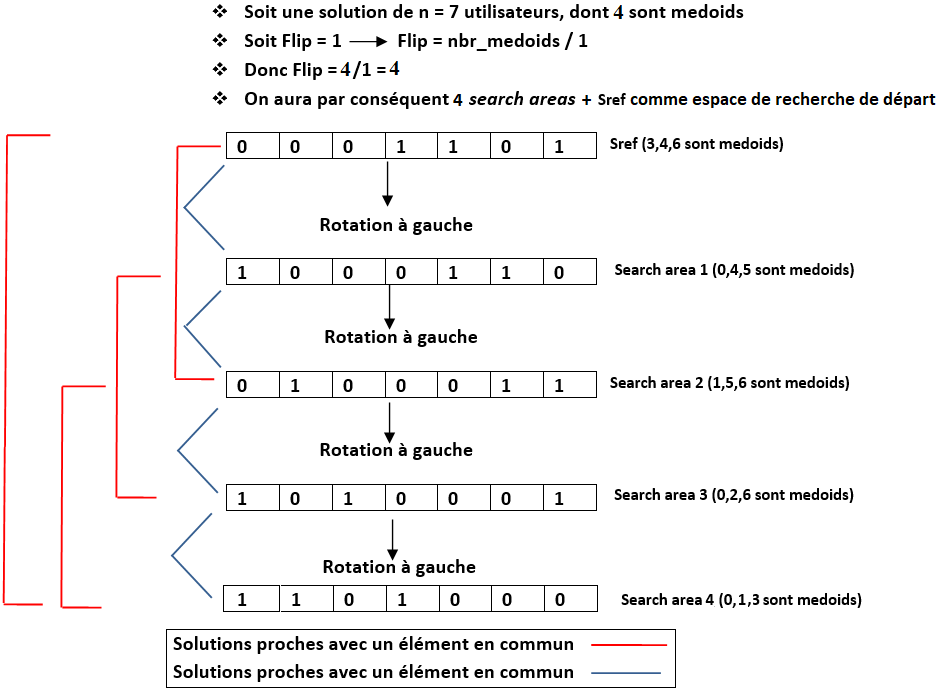
\includegraphics[width=1.1\textwidth]{bsosearch.png}
	\caption{Génération des \textit{search areas} à partir de \textit{Sref}}
	\label{fig:bsosearch}
\end{figure}

\begin{enumerate}[nosep,label=\textbf{\arabic*)}]
	\setcounter{enumi}{4}
	\item \textbf{Fonction fitness}
\end{enumerate}\mbox{}\indent Pour évaluer la qualité du vecteur de solution on a besoin d'évaluer la qualité de la prédiction effectuée à partir du clustering de K-medoids, pour cela nous avons utilisé les métriques RMSE/MAE (à minimiser).
\begin{equation}\label{eq:1}
RMSE = \sqrt{\frac{\sum_{i=1}^{N} (Predicted_{i} - Actual_{i})^{2}  } {N}}  
\end{equation}

\begin{equation}
MAE= \frac {1}{N} \sum_{i=1}^{N} | Predicted_{i} -  Actual_{i}|
\end{equation}

\mbox{}\\Où: 
\begin{itemize}
	\item $Predicted_{i}$: rating prédit pour l'item $i$.
	\item $Actual_{i}$: réel rating  pour l'item $i$.
	\item $N$: nombre d'item total.
\end{itemize}

\begin{enumerate}[nosep,label=\textbf{\arabic*)}]
	\setcounter{enumi}{5}
	\item \textbf{La recherche locale}
\end{enumerate}\mbox{}\indent La recherche locale est effectuée sur chaque vecteur de solution, pour essayer de trouver le nième medoid optimal. 
Une itération de la recherche locale est décrite comme suit:
\begin{enumerate}
	\item Ajouter le nième medoid en changeant la première valeur égale à zéro rencontrée dans le vecteur à un.
	\item Évaluer l'ajout du medoid avec la fonction fiteness, et enregistrer l'évaluation dans une liste nommée \textit{Liste{\_}Eval}.
	\item Défaire l'ajout du nième medoid de l'étape (1).
	\item Refaire les étapes  (1) (2) et (3) pour le reste des valeurs égale à zéro du vecteur solution.
\end{enumerate}
\indent Après avoir terminer le parcours du vecteur solution, on récupère l'indice du medoid qui a donné la meilleure valeur de fonction fitness à partir de \textit{Liste{\_}Eval}, nous affectons à \textit{Sref} la nouvelle solution trouvée dans la recherche locale, et si \textit{nbriterations} n'est pas atteint, alors nous générons des solutions à partir de \textit{Sref} et nous re-effectuant une recherche locale, sinon on sort avec la meilleure solution qui est \textit{Sref}.

\subsubsection*{Calcul de prédiction pour le filtrage avec classification et classification optimisée}Pour la prédiction en se basant sur le vote du cluster auquel appartient chaque utilisateur afin de calculer les ratings des items non encore évalués, et cela en utilisant la formule de la somme pondérée citée précédemment.

\section{Exemple de calcul de prédiction}
Soit la matrice d'usage suivante:
\begin{figure}[H]
	\centering
	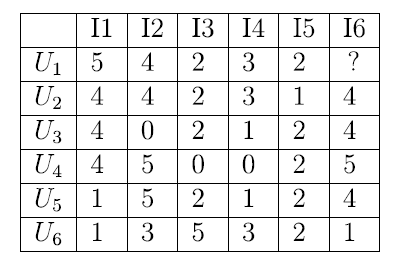
\includegraphics[width=0.40\textwidth]{exemple.PNG}
	\caption{Exemple de matrice d'usage}
	\label{fig:exemple}
\end{figure}
Pour calculer les distances entre les utilisateurs en applique la formule de distance de Pearson suivante:
\begin{equation}
pearson(u,v)= 1 - \frac{\sum_{i \in I} (r_{u,i}-\bar{r}_{u}).(r_{v,i}-\bar{r}_{v})}{\sqrt{\sum_{i \in I} (r_{u,i}-\bar{r}_{u})^{2}.(r_{v,i}-\bar{r}_{v})^{2}}}
\end{equation}
On aura la matrice de distance entre utilisateur comme suit:

\begin{figure}[H]
	\centering
	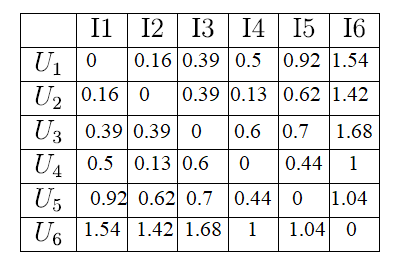
\includegraphics[width=0.45\textwidth]{exemplesim.PNG}
	\caption{Exemple de matrice de distance}
	\label{fig:sim}
\end{figure}

Pour calculer la prédiction de l'utilisateur $U_{1}$ sur l'item $I_{6}$, on effectue tout d'abord un des types de filtrage conçu pour trouver les voisins de chaque utilisateur, on suppose que les voisins de l'utilisateur $U_{1}$ sont comme suit:
 
\begin{figure}[H]
	\centering
	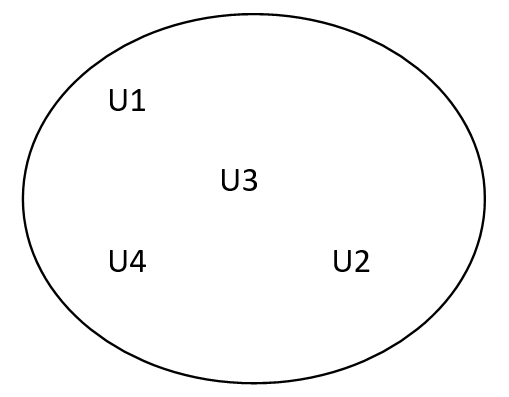
\includegraphics[width=0.35\textwidth]{voisin.PNG}
	\caption{Les voisins de l'utilisateur $U_{1}$}
	\label{fig:voisin}
\end{figure}
En utilisant la formule de prédiction de somme pondérée suivante:
\begin{equation}
pred(u_{i},i_{k})=\bar{r(u_{i})} + \frac{\sum_{u_{j} \in U_{i}} sim(u_{i},u_{j}).(r_{u_{j,ik}}-\bar{r(u_{j})})}{\sum_{u_{j} \in U_{i}} sim(u_{i},u_{j})}
\end{equation}
On aura:
\begin{equation}
pred(u_{1},i_{6})=	3.2 + \frac{0.16 * (4-3) + 0.39 * (4-2.6) + 0.5 * ( 5-4)}{ 0.16 + 0.39 + 0.5}= 4.38
\end{equation}
\section {Ingénierie du système}
Nous présentons le diagramme de cas d'utilisation qui modélise les différentes fonctionnalités de notre système de recommandation.
\begin{figure}[H]
	
	\centering
	\hspace*{-0.85in}
	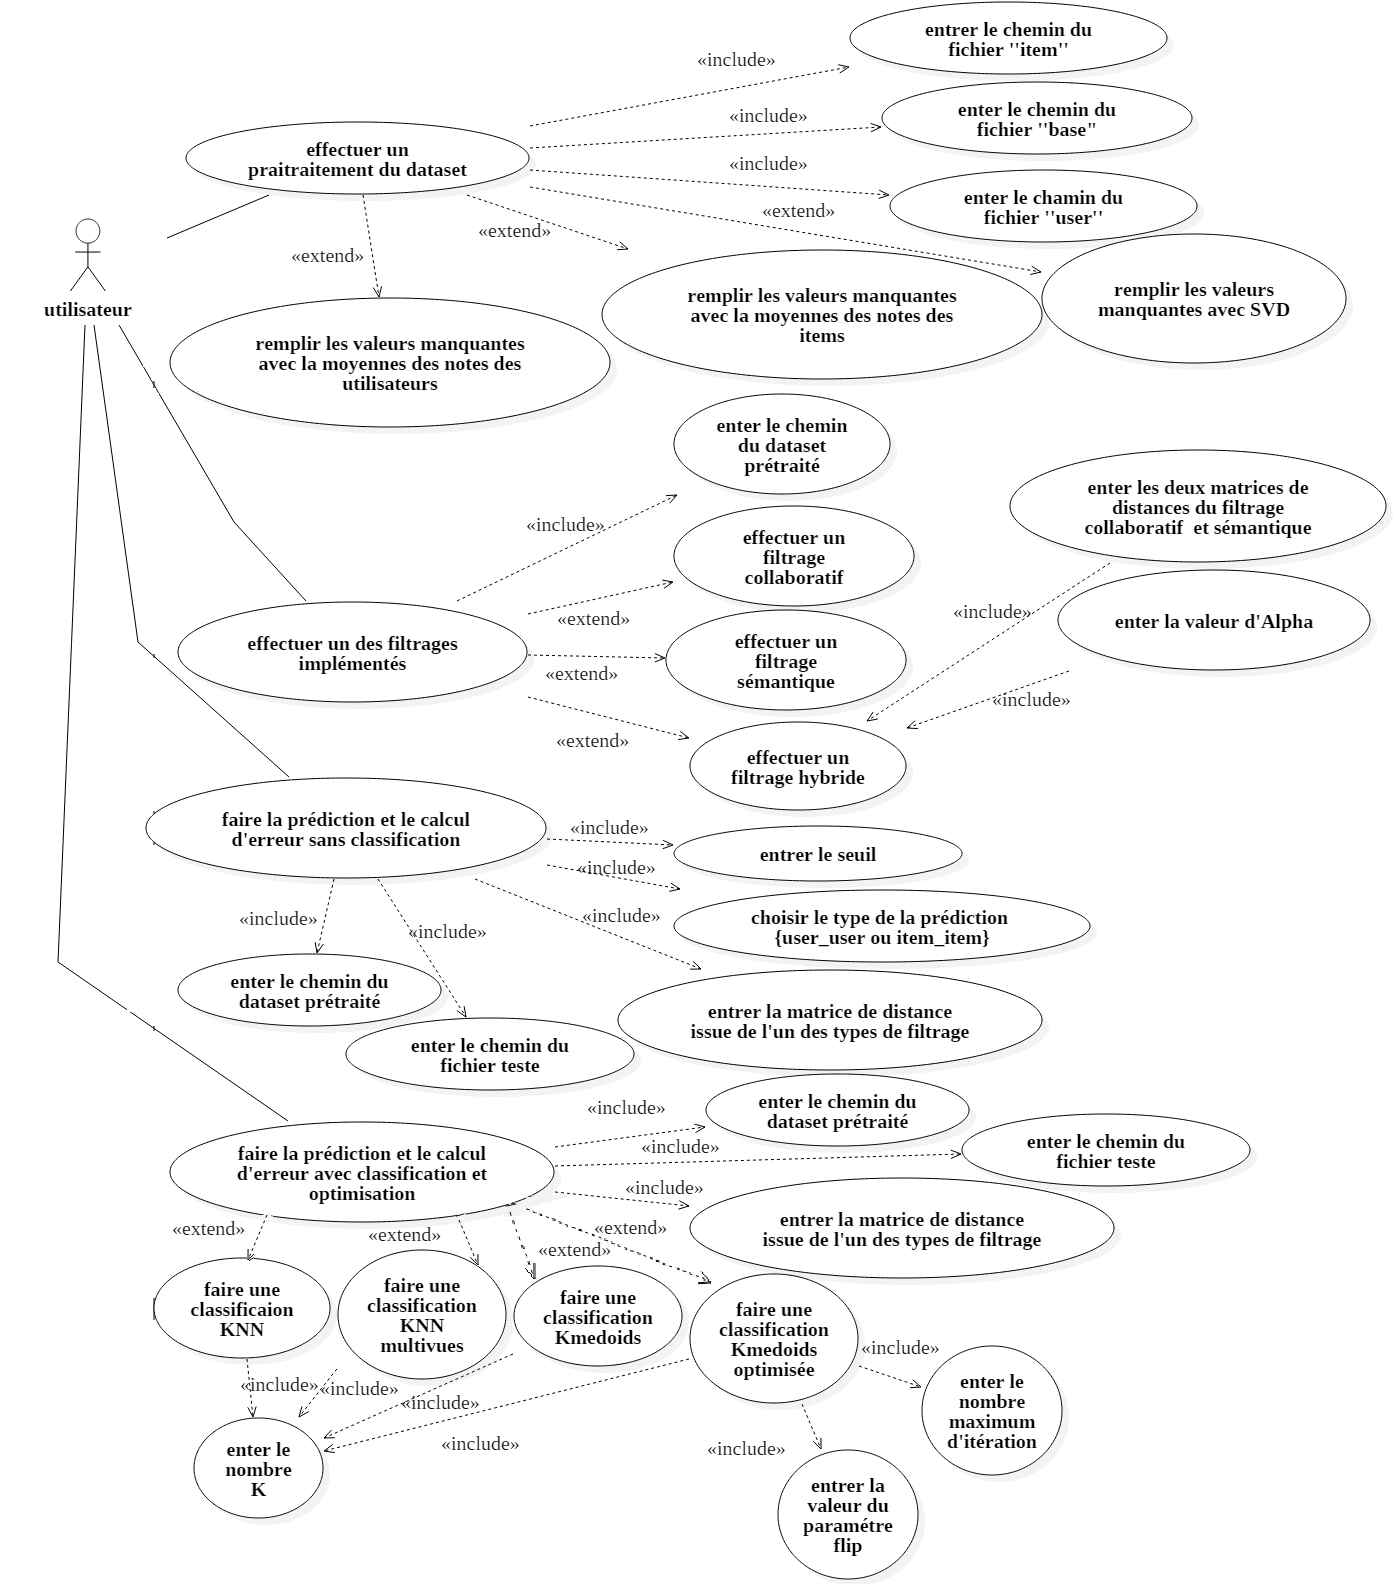
\includegraphics[width=1.2\textwidth]{shemaglobalesys.PNG}
	
	\caption{Diagramme de cas d'utilisation de notre système de recommandation}
	
	\label{fig:shemaglobalesys}
	
\end{figure}
\section {Conclusion}
Dans ce chapitre nous avons présenté en détail notre approche de recommandation qui utilise trois types de filtrage: Collaboratif, sémantique et hybride (combinant ces deux algorithmes selon différentes méthodes). Dans un second lieu, nous avons appliqué deux techniques de classification, supervisée (L'algorithme KNN a été utilisé) et non supervisée (l'algorithme K-medoids a été utilisé). Une hybridation basé sur ces algorithmes a été considéré, dont l'hybridation multivues avec KNN. Finalement, afin d'améliorer la qualité de la classification, nous avons appliqué une optimisation en utilisant la métaheuristique BSO (algorithme K-medoids-BSO). 
Dans le chapitre suivant nous allons évaluer notre système de recommandation et présenter l'interface réalisée qui permet aux utilisateurs de tester notre système et de visualiser les résultats obtenus.

\chapter{Implémentation et expérimentation }
\thispagestyle{empty}
\newpage
\section{Introduction}
Dans le chapitre précédent, nous avons proposé une approche de recommandation incluant plusieurs algorithmes basés sur des techniques différentes (hybridation, clustering, clustering optimisé et clustering multivues). 
Dans ce chapitre, nous présenterons en détail l'implémentation et l'expérimentation de notre système de recommandation.
Ce chapitre est structuré comme suit:
\begin{itemize}
	\item L'environnement de travail (langage, outils et bibliothèques utilisés),
	\item L’application réalisée, (son fonctionnement et mode d’emploi),
	\item L'analyse des performances de l’approche développée et la comparaison de nos résultat avec ceux d’autres techniques déjà existantes.
\end{itemize}

\section{Environnement de travail}
Nous allons présenter dans cette partie les outils que nous avons utilisé pour réaliser notre système de recommandation.
\subsection{Langage de programmation \textit{Python}}
Créé originellement par le programmeur Guido van Rossum autour de 1990, \textit{Python} est un langage de programmation objet interprété de haut niveau avec une sémantique dynamique. Ses structures de données intégrées de haut niveau, combinées à un typage et liaison dynamique, le rendent très attrayant pour le développement rapide d'applications, ainsi que pour son utilisation en tant que langage de script ou de collage pour connecter des composants existants\cite{ref39}.


\myparagraph{Caractéristiques du langage et avantages}
\begin{itemize}
	\item La syntaxe simple et facile à apprendre de Python met l'accent sur la lisibilité et réduit donc le coût de la maintenance du programme. 
	\item Python prend en charge les modules et les packages, ce qui encourage la modularité du programme et la réutilisation du code. 
	\item L'interpréteur Python et la vaste bibliothèque standard sont disponibles gratuitement sous forme binaire ou source pour toutes les principales plates-formes et peuvent être distribués librement.
\end{itemize}

\subsection{Outils et logiciels}
\myparagraph{Système d’exploitation (Linux)}Linux est un noyau monolithique à code source ouvert. Le noyau Linux a été développé à l'origine par Linus Torvalds, qui l'a annoncé dans le groupe de discussion comp.os.minix le 25 août 1991. Depuis lors, il a été porté sur des architectures informatiques comprenant x86-64, x86, ARM, RISC et DEC Alpha. Les développeurs ont accès à tout le code source de Linux et sont autorisés, dans les conditions de la licence, à le modifier et à le distribuer \cite{ref40}.

\myparagraph{L’environnement de développement (Visual Studio
Code)}
Visual Studio Code est un éditeur de code source gratuit et libre de droit, disponible pour Windows, macOS et Linux. Il est livré avec un support intégré pour JavaScript, TypeScript et Node.js et dispose d'un écosystème riche en extensions pour d'autres langages (tels que C ++, C\#, Java, Python, PHP, Go) \cite{ref41}.

\section{Présentation de notre système de recommandation}
\subsection{Description générale}
Le système que nous avons développé permettra de lancer les différents
algorithmes implémentés et de visualiser en détails les performances et les résultats de chaque technique stockés dans des fichiers \textit{.csv}.

Il sera également possible de choisir le dataset (jeux de données) à utiliser. Toutes les techniques implémentées sont généralisées pour traiter n’importe quel dataset possédant la structure montrée dans la figure \ref{fig:shemfi}.
La modularité du code source de l’application permettra facilement d’apporter des mises à jours aux algorithmes afin d'ajouter d'autre techniques.
\begin{figure}[H]
	\centering
	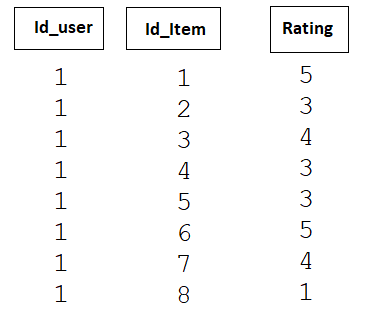
\includegraphics[width=0.5\textwidth]{shemfi.PNG}
	\caption{Exemple de structuration d'un fichier exploitable dans notre système de recommandation}
	\label{fig:shemfi}
\end{figure}



\subsection{Illustration des fonctionnalités développées}
L'interface de l'application est composée de 4 onglets, qui sont:
\begin{itemize}
	\item\textit{Data preprocessing}: le prétaitement des données d'un dataset est une étape essentielle avant son utilisation, dans notre cas il existe énormément de valeurs manquantes de rating  car les users ne notent pas tous les items existants et par conséquent la prédiction effectuée ne sera pas précise.
	Pour effectuer un prétraitement du dataset, il faut passer en entrée trois fichiers, qui sont: 
	\begin{itemize}
		\item Fichier \textit{u.item}: contient les identificateurs des items.
		\item Fichier \textit{u.user}: contient les identificateurs des utilisateurs.
		\item Fichier \textit{u.base}: contient les évaluations faites par les utilisateurs sur les items.
	\end{itemize}
	Le traitement des valeurs manquantes s'effectue avec l'une des options suivantes:
	\begin{itemize}
		\item Moyenne de rating des utilisateurs: on remplace les valeurs manquantes en effectuant la moyenne des évaluations des utilisateurs, pour voir en général la note que ces derniers attribuent aux items.
		
		\item Moyenne de rating des items: les valeurs manquantes d'un item sont remplacées par la moyenne des évaluations qu'il lui sont attribuées.
		
		\item SVD: nous utilisons la technique SVD expliqué dans le chapitre 3, afin d'effectuer une décomposition de la matrice d'usage du dataset pour extraire les caractéristiques cachées des items et des utilisateurs et ainsi les faire correspondre selon leurs caractéristiques, et remplacer les valeurs manquantes des ratings.
		
		On note qu'on peut laisser le fichier tel quel sans prétraitement.
	\end{itemize}

Quand le prétraitement des données est effectué, le résultat est sauvegardé dans un fichier pour une exploitation ultérieure.


\begin{figure}[H]
	\centering
	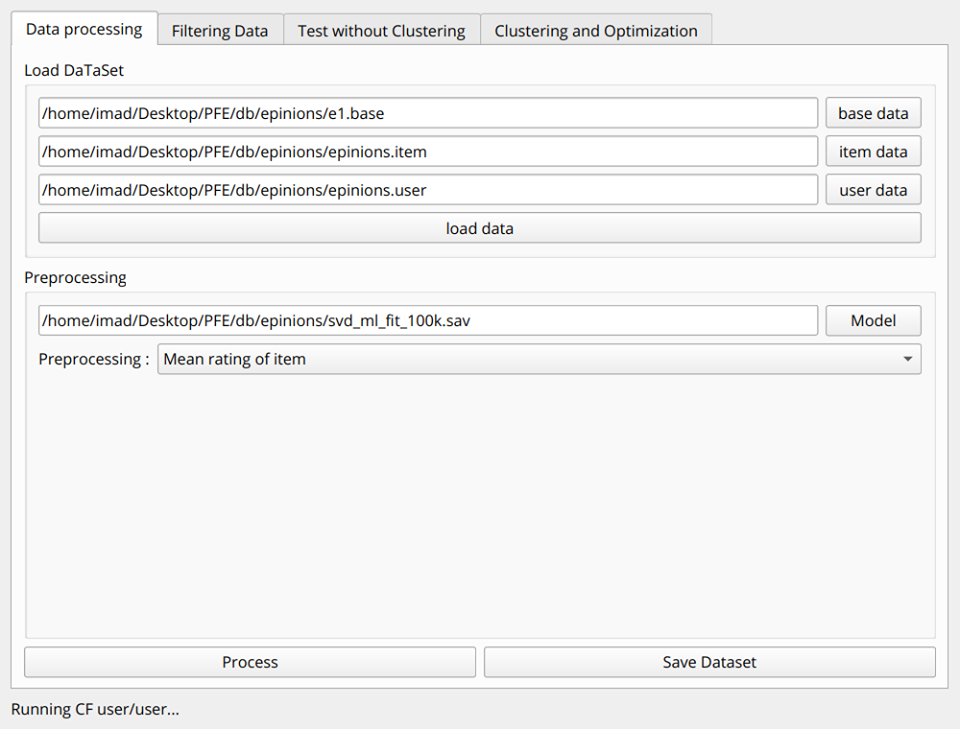
\includegraphics[width=\textwidth]{datapre.PNG}
	\caption{Capture d'écran de l'onglet \textit{Data preprocessing}}
	\label{fig:datapre}
\end{figure}

	\item \textit{Filtering data}: dans cet onglet on effectue l'un des filtrage conçu (FC, FSem, hybride), le fichier prétraité dans l'étape précédent est importé puis le calcul des distances entre les utilisateurs s'effectue avec les formules de similarité des filtrage et le résultat est sauvegardé dans un fichier (stockage de la matrice des distances dans un fichier).
	
	\begin{figure}[H]
		\centering
		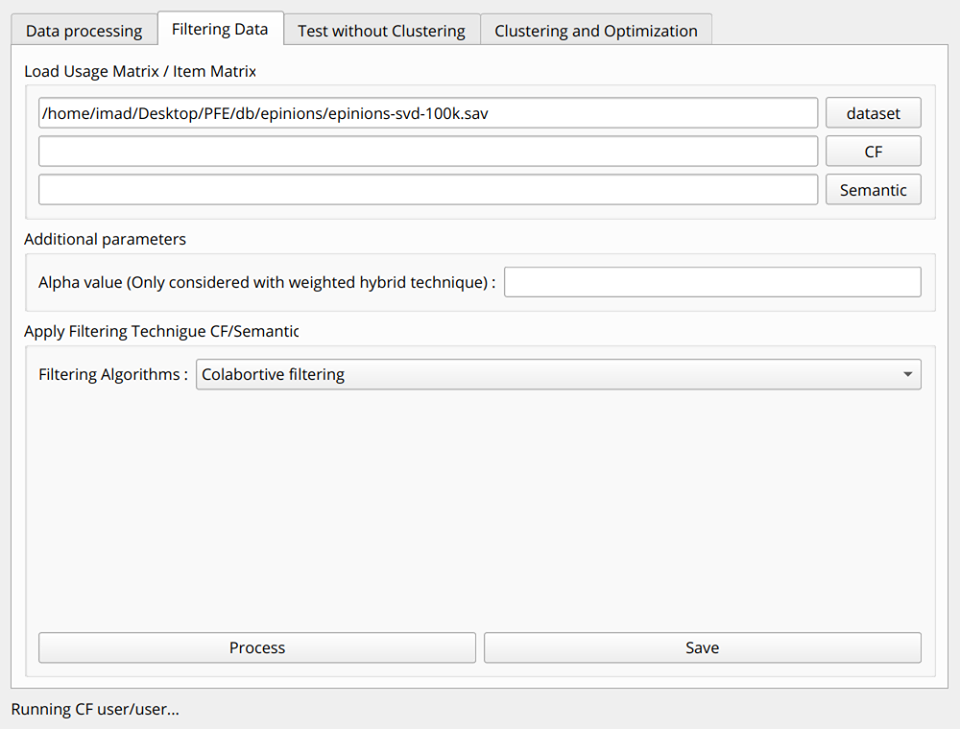
\includegraphics[width=\textwidth]{filter.PNG}
		\caption{Capture d'écran de l'onglet \textit{Filtering data}}
		\label{fig:filter}
	\end{figure}
	\item \textit{Test without classification}: comme expliqué dans le chapitre précédent, après avoir obtenu la matrice de distances qui est issue de l'un des types de filtrage on peut effectuer les prédictions des évaluations des items en utilisant un seuil qui permet la sélection des voisins des utilisateurs (ou les items pour le cas FC item-item).
	On commence par introduire le fichier prétraité d'un dataset, car il contient les évaluations des items donnés par les users, puis la matrice de distance du dataset pour la sélection des voisins des users. Le type de la matrice de distance qu'on introduit dépend des cas suivant:
	\begin{itemize}
		\item Si FC item-item alors introduire matrice de distance item-item calculée avec formule de Pearson.
		\item Si FC user-user alors introduire matrice de distance user-user calculée avec formule de Pearson.
		\item Si FSem alors introduire matrice de distance user-user calculée avec formule distance d'interet.
		\item Si filtrage hybride alors introduire matrice de distance hybride calculée avec formule Pearson et distance d'intérêt.
	\end{itemize}
	
	Après avoir importer les fichier du dataset prétraité et sa matrice de distance, on importe le fichier test qui contient les ratings des items pour effectuer les prédictions et vérifier la qualité de cette dernière avec les métriques RMSE et MAE vus dans le chapitre précédent et les affichées dans l'interface.
	
	\begin{figure}[H]
		\centering
		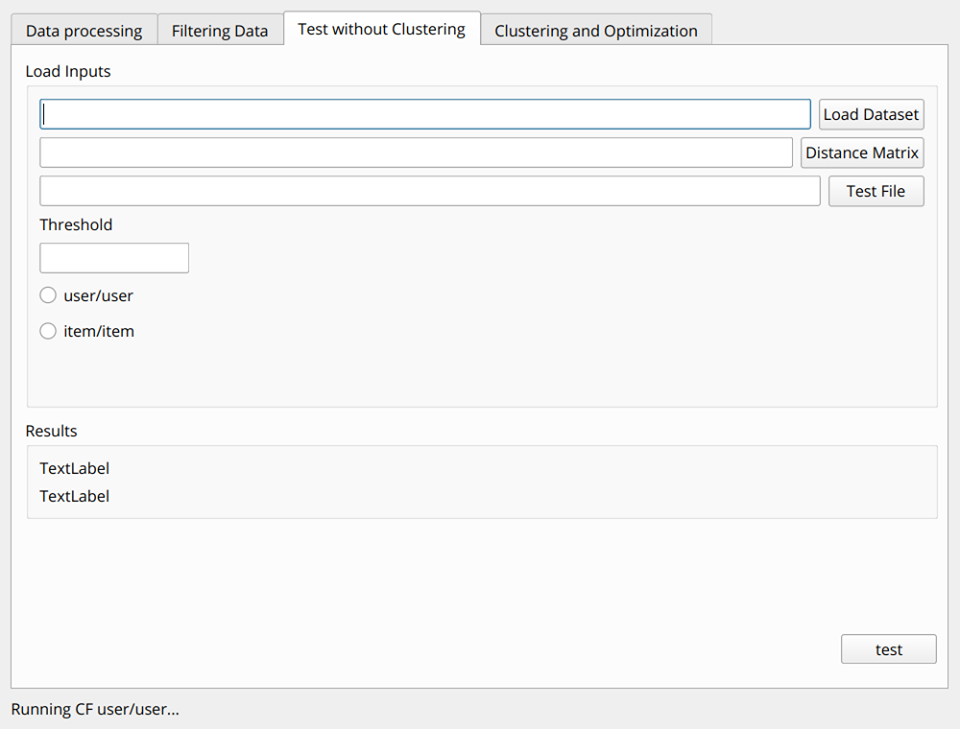
\includegraphics[width=\textwidth]{sansclus.PNG}
		\caption{Capture d'écran de l'onglet \textit{Test without classification}}
		\label{fig:sansclus}
	\end{figure}
	\item \textit{Classification and optimisation}: pour faire un filtrage avec classification ou classification optimisée,  les mêmes étapes de l'onglet \textit{test without clustering} sont reeffectuées sauf qu'au lieu d'introduire un seuil de sélection de voisins, on utilise un algorithme de classification sur la matrice de distances des users (respectivement des items pour le FC item-item avec classification).
	Après avoir introduit les fichiers contenant le dataset, la matrice de distances et les items de test, on entre les paramétrés selon la technique de classification voulue:
	
	\begin{itemize}
		\item K-medoids: le nombre K de cluster est requis pour lancer une classification avec K-medoids des utilisateurs.
		\item K-medoids optimisé: le nombre K de cluster à former et \textit{max iterations} qui est le nombre maximum d'itération à effectuer pour trouver une solution optimisée.
		\item K-NN: le nombre K de voisins à considérer pour les prédictions des ratings de chaque utilisateur.
		\item K-NN multiview: (le même paramètre que K-NN est requis pour exécuter K-NN multiview).
	\end{itemize} 
	Les résultats des évaluations des prédictions sera affiché après exécution des algorithmes dans l'interface est qui sont: RMSE, MAE, rappel, précision. 

\begin{figure}[H]
	\centering
	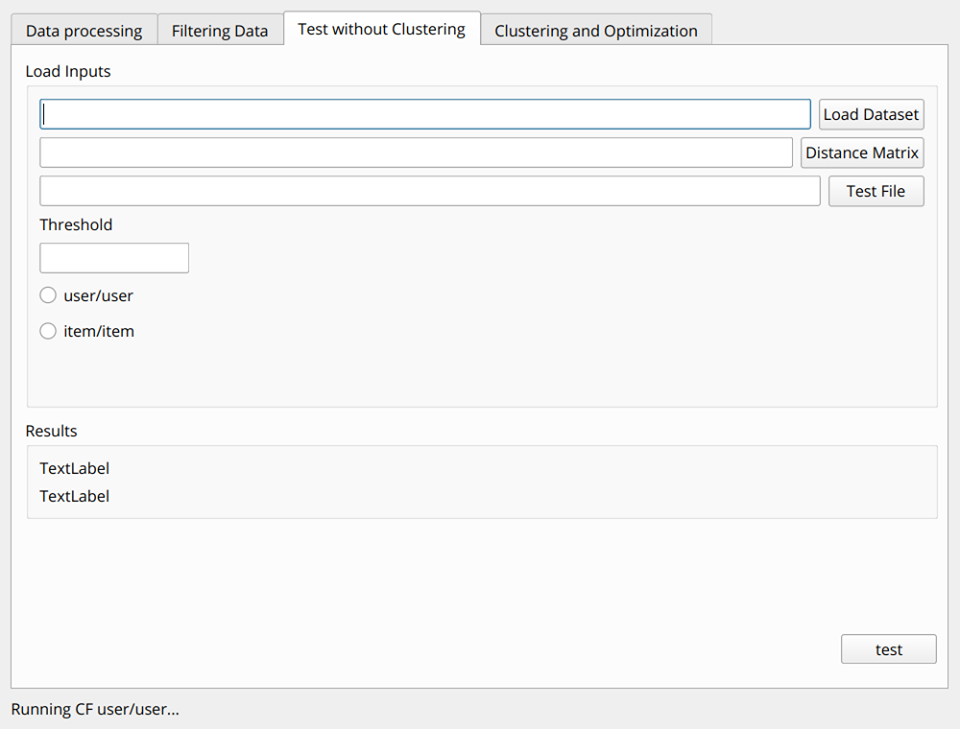
\includegraphics[width=\textwidth]{sansclus.PNG}
	\caption{Capture d'écran de l'onglet \textit{Classification and optimisation}}
	\label{fig:clasificationonglet}
\end{figure}


\end{itemize}



\section{Expérimentation}
\subsection{Dataset}
\begin{enumerate}[nosep,label=\textbf{\arabic*)}]
	%%\setcounter{enumi}{2}
	\item \textbf{Présentation de \textit{MovieLens}}
\end{enumerate}\mbox{} \indent GroupLens Research (un laboratoire de recherche de l’université du Minnesota) a mis à disposition un ensemble de données d’évaluation à partir du site Web MovieLens collectés sur différentes périodes.
On retrouve des jeux de données allant de 100 000 évaluations jusqu'à 20 millions, ce dernier est plus destinées à la recherche ou de grand moyens matériels sont souvent nécessaires.
Étant limité par le temps et par la puissance de calcul de nos machines, nous
opterons donc dans un premier temps pour des dataset de 100 000 évaluations afin d’effectuer nos tests.

\myparagraph{Architecture du dataset}Le dataset \textit{100K} de \textit{MovieLens} se présente sous la structure suivante :
\begin{itemize}
	\item Un fichier \textit{u.data}: de 100 000 lignes, contenant l’ensemble des évaluations (l’id de l’utilisateur, l’id de l’item, l’évaluation (de 1 à 5), la date d’évaluation).
	\item  Un fichier \textit{u.genre}: ou on peut retrouver les différent catégories des films présents sur la plate-forme.
	\item  Un fichier \textit{u.item}: ou sont indiqués tous les films avec l’ensemble des informations qui leurs sont relatives : date de sortie, genre etc ...
	\item Un fichier \textit{u.occupation}: indiquant les différentes professions des utilisateurs.
	\item  Un fichier \textit{u.user}: contenant les informations relatives à chaque utilisateur: age, sexe, profession etc ...
	\item  Un fichier \textit{u.base}: contient 80\%  des données \textit{u.data}, ce fichier est utilisé pour effectuer l'apprentissage (classification et construction de modèle).
	\item  Un fichier \textit{u.test}: contient 20\%  des données \textit{u.data}, ce fichier est utilisé pour effectuer les testes (prédiction et calcule d'erreur).
\end{itemize}
\subsubsection*{Exploitation du dataset}
Le processus de test et d’évaluation d’un algorithme nécessite deux ensembles de données : un ensemble d’apprentissage et un ensemble de test.
En effet, l’ensemble de données du fichier \textit{u.data} contient en tout 100 000 évaluations, nous prendrons donc \textit{u.base} qui contient 80 000 évaluations pour l’apprentissage et \textit{u.test} qui contient 20 000 évaluations pour la prédiction et le calcul des métriques.

\begin{enumerate}[nosep,label=\textbf{\arabic*)}]
	\setcounter{enumi}{1}
	\item \textbf{Présentation de \textit{RED}}
\end{enumerate}\mbox{} \indent Epinions.com était un un site général d'évaluation des consommateurs créé en 1999. Epinions a été acquis par Shopping.com (connu sous le nom de DealTime au moment de l'acquisition) en 2003, qui a ensuite été acquis par eBay en 2005. Chez Epinions, les visiteurs pouvaient lire nouvelles et anciennes critiques sur une variété d’articles pour les aider à effectuer leurs achats. Le 25 mars 2014, toutes les fonctionnalités de la communauté, ainsi que les fonctionnalités de soumission et de modification des avis, ont été désactivées. Par la suite, en mai 2018, le site a été complètement fermé et les URL du domaine epinions.com sont redirigées vers Shopping.com.

RED: (\textit{Rich Epinions Dataset for Recommender Systems}) est un jeu de données extrait d'Epinions et enrichi. Il contient des critiques d'utilisateurs sur les éléments, les valeurs de confiance entre les utilisateurs, la catégorie d'éléments, la hiérarchie des catégories et l'expertise des utilisateurs sur les catégories. Cet ensemble de données peut être utilisé pour évaluer divers systèmes de recommandation.

\myparagraph{Architecture du dataset}
Le dataset est une base de données relationnelle avec les tables suivantes:
\begin{itemize}
	\item Utilisateur: nom (pseudo et URL du profil), location, rang (peut être nul) et les visites de profil.
	\item Item: nom, catégorie et URL du profil.
	\item  Catégorie: nom, catégorie parent, url de description, lignage (chemin dans l'arborescence des catégories) et profondeur (dans l'arborescence des catégories).
	\item Critique: une critique associe un utilisateur à un élément, elle contient la note, entre 1 et 5, la note de la revue (moyenne de toutes les notes associées à cette critique) et la date de révision.
	\item Expertise: les utilisateurs experts dans une catégorie apparaissent ici avec l'expertise (responsable de la catégorie, examinateur principal, conseiller) associée à la catégorie considérée.
	\item Trust: Web de confiance, c’est-à-dire une valeur de confiance (-1 ou 1) d’un utilisateur à un autre, seules les valeurs de confiance positives apparaissent dans le jeu de données.
	\item Similarité: la similarité entre tous les couples d'utilisateurs avec la corrélation de coefficient de Pearson. 
\end{itemize}

\begin{figure}[H]
	\centering
	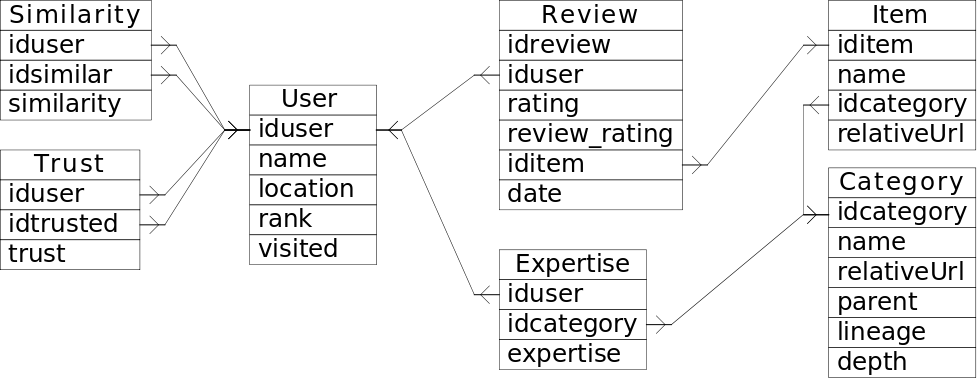
\includegraphics[width=\textwidth]{shemata.PNG}
	\caption{Architecture de la base de données RED}
	\label{fig:shemta}
\end{figure}
\subsubsection*{Exploitation du dataset}
Nous avons pris un échantillon du dataset RED, qui est formé de 100K ratings de 149 utilisateurs sur 5000 items, et nous avons divisé cette échantillon en deux ensemble de données, un ensemble d'apprentissage environ 80\% de l'échantillon et un ensemble de 20\% pour les testes. 
\subsection{Métriques d'évaluation}
Nous nous baserons sur deux métriques afin d’évaluer notre travail : MAE et RMSE cité dans le chapitre précédant (voir formule \ref{eq:1}), qui sont des métriques permettant de calculer la différence
entre deux variables continues. En effet, ces deux métriques restent les plus utilisées dans le domaine et les plus pertinentes quant à évaluer la qualité d’un système de recommandation.

\subsection{Résultats des évaluations}
Dans cette partie, nous réaliserons un ensemble de tests portant sur les performances de notre approche et nous comparerons nos résultats avec les résultats des approches existantes. 
\textbf{A) Évaluations avec MovieLens-100K}
\begin{enumerate}[nosep,label=\textbf{\arabic*)}]
	%%  \setcounter{enumi}{4}
	\item \textbf{Filtrage collaboratif}
\end{enumerate}
\subsubsection*{FC sans classification}
Dans cette phase d’expérimentations, nous allons évaluer la qualité de la recommandation lorsque celle-ci est basée sur un filtrage collaboratif standard (user-user, item-item, SVD). Nous ferons des expérimentations par rapport à la corrélation de Pearson, étant donné que celle-ci reste l’une des plus connues et des plus utilisées.
Nous avons évalué les algorithmes suivants:
\begin{itemize}
	\item  FC item-item avec un praitrétement la moyenne des évaluations des utilisateur 
	(FC-item-item-UA).
	\item  FC item-item avec un praitrétement la moyenne des évaluations des items (FC-item-item-IA).
	\item  FC item-item avec un praitrétement la méthode SVD (FC-item-item-SVD).
	\item FC item-item sans prétraitement (FC-item-item).
	\item  FC user-user avec un praitrétement la moyenne des évaluations des utilisateur (FC-user-user-UA).
	\item  FC user-user avec un praitrétement la moyenne des évaluations des items (FC-user-user-IA).
	\item  FC user-user avec un praitrétement la méthode SVD (FC-user-user-SVD).
	\item FC user-user sans prétraitement (FC-user-user).	
\end{itemize}
\begin{figure}[H]
	\centering
	\includegraphics[width=\textwidth]{MAEFC.PNG}
	\caption{Évaluation MAE du FC standard en fonction du seuil}
	\label{fig:FCMAE}
\end{figure}

\begin{figure}[H]
		\centering
	\includegraphics[width=\textwidth]{RMSEFC.PNG}
	\caption{Évaluation RMSE du FC standard en fonction du seuil}
	\label{fig:FCRMSE}
\end{figure}

\begin{center}\label{tab1}
	\begin{tabularx}{\textwidth}{|p{3.7cm}|l|l|l||p{3.65cm}|l|l|l|}
		\hline
		threshold & 0.258 & 0.345 & 0.301 & threshold & 0.073 & 0.109 & 0.256 \\ \hline
		MAE  (FC-item-UA) & 0.796 & 0.797 & 0.798 & MAE  (FC-user-IA) & 0.798 & 0.799 & 0.8 \\ \hline
		RMSE (FC-item-UA) & 1.067 & 1.067 & 1.068 & RMSE (FC-user-IA) & 1.069 & 1.07 & 1.07 \\ \hline\hline
		threshold & 0.284 & 0.227 & 0.17 & threshold & 0.4 & 0.6 & 0.5 \\ \hline
		MAE  (FC-user-SVD) & \textbf{0.73} & 0.736 & 0.75 & MAE  (FC-item-IA) & 0.775 & 0.78 & 0.782 \\ \hline
		RMSE (FC-user-SVD) & \textbf{1.001} & 1.007 & 1.023 & RMSE (FC-item-IA) & 1.064 & 1.066 & 1.07 \\ \hline\hline
		threshold & 0.454 & 0.606 & 0.53 & threshold & 0.151 & 0.227 & 0.303 \\ \hline
		MAE  (FC-user-ua) & 0.761 & 0.78 & 0.781 & MAE  (FC-user-user) & 0.795 & 0.81 & 1.022 \\ \hline
		RMSE (FC-user-ua) & 1.047 & 1.066 & 1.066 & RMSE (FC-user-user) & 1.079 & 1.111 & 1.492 \\ \hline\hline
		threshold & 0 & 0.105 & 0.158 & threshold & 0 & 0.1 & 0.2 \\ \hline
		MAE  (FC-item-SVD) & 0.923 & 0.93 & 0.94 & MAE  (FC-item-item) & 0.804 & 0.808 & 0.829 \\ \hline
		RMSE (FC-item-SVD) & 1.197 & 1.207 & 1.217 & RMSE (FC-item) & 1.076 & 1.085 & 1.133 \\ \hline
	\end{tabularx}	
	\captionof{table}{Récapitulatif des trois meilleurs résultats (MAE et RMSE) pour chaque FC sans classification} 
\end{center}
\subsubsection*{Discussion des résultats}
En analysant les deux figures ci-dessus, il est clair qu’au delà d’un certain seuil, environ 0.5, la qualité de la prédiction stagne pour les différent types de FC.

On remarque que lorsque le dataset n'est pas prétraité les résultats sont de qualité médiocre, ce qui confirme l'importance du prétraitement du dataset, les meilleures valeurs de MAE et RMSE sont au alentour de respectivement 0.80 et 1.2 dans le cas de FC user-user et FC item-item.

Les deux filtrages collaboratif user-user avec comme prétraitement la moyennes des items (FC-user-user-IA) et FC item-item avec  prétraitement la moyenne des users (FC-item-item-UA), donnent des résultat presque similaire environ  0.79 pour le meilleur MAE et 1.06 pour RMSE.
 
L'utilisation de la technique de SVD pour le prétraitement et l'application d'un FC item-item  par la suite (FC-item-item-SVD), donne de très mauvais résultats, donc cette technique est à exclure pour la suite des évaluations avec classification.

Le filtrage qui a donné les meilleures évaluations est FC user-user (FC-user-user-SVD) avec comme prétraitment SVD, et la meilleure valeur de MAE est égale à 0.73 et RMSE égale à 1.001, pour un seuil de 0.284, donc nous allons opté pour ce filtrage dans la suite des évaluations.

\subsubsection*{FC Avec classification}
Pour cette approche, nous ferons varier la valeur de k dans les algorithmes de FC avec classification, et essayer de déduire laquelle de ses valeurs nous permettra d’atteindre les meilleurs résultats.
Nous avons évalué les algorithmes suivants:
\begin{itemize}
	\item  FC user-user basé K-medoids (FC-user-user-Kmedoids).
	\item  FC user-user basé K-medoids et BSO (FC-user-user-Kmedoids-BSO).
	\item  FC user-user basé K-KNN (FC-user-user-KNN).
\end{itemize}

\begin{figure}[H]
		\centering
	\includegraphics[width=\textwidth]{MAEclassFC.PNG}
	\caption{Évaluation MAE du FC avec classification en fonction du seuil}
	\label{fig:MAEclassFC}
\end{figure}


\begin{figure}[H]
		\centering
	\includegraphics[width=\textwidth]{RMSEclassFC.PNG}
	\caption{Évaluation RMSE du FC avec classification en fonction du seuil}
	\label{fig:RMSEclassFC}
\end{figure}
\begin{table}[H]
	\centering
	\begin{tabular}{|l|l|l|l|}
		\hline
		threshold & 0.284 & 0.227 & 0.17 \\ \hline
		MAE  (FC-user-SVD) & \textbf{0.73} & 0.736 & 0.75\\ \hline
		RMSE (FC-user-SVD) & \textbf{1.001} & 1.007 & 1.023 \\\hline \hline
		K & 10 & 15 & 45 \\ \hline
		MAE(FC-kmedoids) & 0.733 & 0.732 & 0.734 \\ \hline
		RMSE(FC-svd-kmedoids) & 1.004 & 1.003 & 1.007 \\ \hline\hline
		K & 25 & 15 & 20 \\ \hline
		MAE(FC-kmedoids-bso) & \textbf{0.728} & 0.729 & 0.73 \\ \hline
		RMSE(FC-kmedoids-bso) & \textbf{1.001} & 1.001 & 1.001 \\ \hline\hline
		K & 50 & 40 & 30 \\ \hline
		MAE(FC-KNN) & 0.73 & 0.731 & 0.732 \\ \hline
		RMSE(FC-KNN) & 1.001 & 1.001 & 1.002 \\ \hline
	\end{tabular}
\captionof{table}{Récapitulatif des trois meilleurs résultats (MAE et RMSE) pour l'algorithme de FC avec classification}
\end{table}
\subsubsection*{Discussion des résultats}
Comme nous pouvons le constater sur les figures \ref{fig:MAEclassFC} et \ref{fig:RMSEclassFC} ci-dessus, la qualité de la prédiction évolue selon le nombre de voisins choisis. En prenant plus de 85 voisins la qualité semble diminuer pour les trois algorithme.

L'ajout du clustering au FC avec comme prétraiement SVD ne semble pas améliorer les résultats car la meilleure valeur de MAE obtenu est 0.733 pour FC basé Kmedoids alors que FC avec SVD elle était égale à 0.73, on suppose que le choix aléatoire des medoids est la cause de la non amélioration des évaluations, de ce fait une optimisation du choix des medoids est nécessaire pour voir l'apport de classification.

Nous pouvons constater que le FC basé Kmedoids-BSO améliore les résultats de FC basé K-medoids et FC standard, avec MAE égale à 0.728, ce qui confirme l'apport de l'optimisation sur le clustering et donc on peut dire que le clustering peut améliorer les résultats d'un FC standard si le jeu de teste est d'un volume plus important.

En ce qui concerne le FC basé K-NN, il n'améliore pas la qualité des évaluations du FC standard mais donne de résultats plus au moins stable avec MAE ne dépassant pas les 0.74 et RMSE les 1.005.

%%%%%%%%%%%%%%%%%%%%%%%FILTRAGE SEMANTIQUE%%%%%%%%%%%%%%%%%%%%%%%%%
\mbox{}\\
\begin{enumerate}[nosep,label=\textbf{\arabic*)}]
	 \setcounter{enumi}{1}
	\item \textbf{Filtrage sémantique standard}
	\end{enumerate}\mbox{} \indent Dans cette phase d’expérimentations, nous allons évaluer la qualité de la recommandation lorsque celle-ci est basée sur un filtrage sémantique. Nous ferons des expérimentations en utilisant la formule de distance d'intérêt entre utilisateur, et la distance de Jaccard entre les items car le dataset MovieLense ne possède pas une représentation sous forme d'ontologie des items.
Le prétraitement des valeurs manquantes est effectué avec la méthode SVD.

\subsubsection*{FSem sans classification}
Nous avons évalué l'algorithme FSem user-user.

\begin{figure}[H]
		\centering
	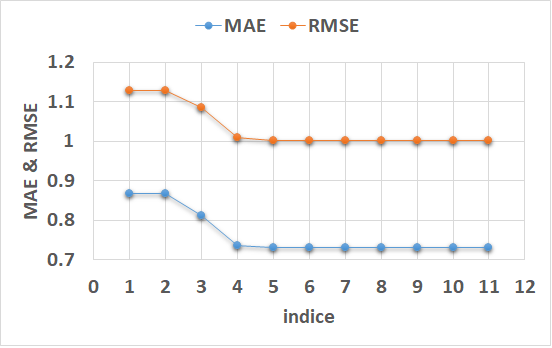
\includegraphics[width=0.8\textwidth]{semsvd.PNG}
	\caption{Évaluation MAE et RMSE du FSem en fonction du seuil de similarité}
	\label{fig:MAEsem}
\end{figure}

Afin de ne pas encombré le graphe ci-dessus (\ref{fig:MAEsem}) nous avons indexé les onze valeurs des seuils du FSem et nous les avons mis dans le tableau suivant:

\begin{table}[H]
	\centering
	\begin{tabular}{|l|l|}
		\hline
		indice & threshold \\ \hline
		1 & 0.6666666666666 564 \\ \hline
		2 & 0.6666666666666 592\\ \hline
		3 & 0.6666666666666 62 \\ \hline
		4 & 0.6666666666666 647 \\ \hline
		5 & 0.6666666666666 675 \\ \hline
		6 & 0.6666666666666 703 \\ \hline
		7 & 0.6666666666666 731 \\ \hline
		8 & 0.6666666666666 758 \\ \hline
		9 & 0.6666666666666 786 \\ \hline
	   10 & 0.6666666666666 814 \\ \hline
	   11 & 0.6666666666666 842 \\ \hline
	\end{tabular}
\captionof{table}{Les valeurs de seuils correspondant aux indices du graphes \ref{fig:MAEsem}}
\end{table}

\begin{center}
	\begin{tabularx}{\textwidth}{|p{5.1cm}|p{3.2cm}|p{3.2cm}|p{3.3cm}|}
		\hline
		indice& 5 & 6 & 9 \\ \hline
		MAE  (FSem-user-user) & \textbf{0.7297} & 0.7306 & 0.7303 \\ \hline
		RMSE (FSem-user-user) & \textbf{1.0012} & 1.0022 & 1.0020\\ \hline
	\end{tabularx}
\captionof{table}{Récapitulatif des trois meilleurs résultats (MAE et RMSE) pour l'algorithme de FSem sans classification}
\end{center}

\subsubsection*{Discussion des résultats}
En analysant la figure \ref{fig:MAEsem} ci-dessus, il est clair qu’au delà d’un certain seuil, plus précisément le seuil possédant l'indice 6, la qualité de la prédiction stagne au alentour de 0.73 pour MAE et 1.002 pour RMSE.

On constate que la meilleure valeur du seuil à choisir dans le FSem standard est le seuil possédant l'indice 5, qui à donné MAE égale à 0.729 et RMSE égale à 1.001.

\subsubsection*{FSem avec classification}
Pour cette approche, nous ferons varier la valeur de K dans les algorithme de FSem avec classification, et essayer de déduire laquelle de ses valeurs nous permettra d’atteindre les meilleurs résultats.
Nous avons évalué les algorithmes suivant:
\begin{itemize}
	\item  FSem user-user basé K-medoids (FSem-user-user-Kmedoids).
	\item  FSem user-user basé K-medoids et BSO (FSem-user-user-Kmedoids-BSO).
	\item  FSem user-user basé K-NN (FSem-user-user-KNN).
\end{itemize}
\begin{figure}[H]
	\centering
	\includegraphics[width=0.9\textwidth]{semMAEclass.PNG}
	\caption{Évaluation MAE avec les algorithmes de FSem basés classification}
	\label{fig:semMAEclass}
\end{figure}

\begin{figure}[H]
	\centering
	\includegraphics[width=0.9\textwidth]{RMSEclasssem.PNG}
	\caption{Évaluation RMSE avec les algorithmes de FSem basés classification}
	\label{fig:RMSEclasssem}
\end{figure}

\begin{center}\label{tab2}
	\begin{tabularx}{\textwidth}{|p{5.1cm}|p{3.2cm}|p{3.2cm}|p{3.3cm}|}
	\hline
	indice & 5 & 6 & 9 \\ \hline
	MAE  (FSem-user-user) & \textbf{0.7297} & 0.7306 & 0.7303 \\ \hline
	RMSE (FSem-user-user) & 1.0012 & 1.0022 & 1.0020\\ \hline	
	\hline
	k & 10 & 15 & 20 \\ \hline
	MAE  (FSem-user-user-kmedoids-bso) & 0.728 & 0.7292 & 0.7293 \\ \hline
	RMSE (FSem-user-user-kmedoids-bso) & 1.002 & 1.0012 & 1.005 \\ \hline\hline
	k & 55 & 65 & 60 \\ \hline
	MAE  (Fsem-user-user-KNN) & \textbf{0.7297} & 0.7299 & 0.7301 \\ \hline
	RMSE (Fsem-user-user-KNN) & \textbf{1.0007} & 1.0006 & 1.0003 \\ \hline\hline
	k & 15 & 25 & 10 \\ \hline
	MAE  (FSem-user-user-kmedoid) & 0.7301 & 0.7307 & 0.7309 \\ \hline
	RMSE (FSem-user-user-kmedoid) & 1.0012 & 1.0027 & 1.002 \\ \hline
\end{tabularx}
\captionof{table}{Récapitulatif des trois meilleurs résultats (MAE et RMSE) pour l'algorithme de FSem avec classification}
\end{center}

\subsubsection*{Discussion des résultats}
Comme nous pouvons le constater sur les figures \ref{fig:semMAEclass} et \ref{fig:RMSEclasssem} ci-dessus, la qualité de la prédiction évolue selon le nombre de voisins choisis. En prenant plus de 85 voisins la qualité semble diminuer pour les trois algorithme.

L'ajout du clustering au FSem avec comme prétraiement SVD ne semble pas améliorer les résultats car la meilleure valeur de MAE obtenu est 0.730 pour FSem basé Kmedoids, alors que le FSem standard avait donné MAE égale à 0.729, on suppose que le choix aléatoire des medoids est la cause de la non amélioration des évaluations, de ce fait une optimisation du choix des medoids est nécessaire pour voir l'apport de classification.

Après l'ajout de l'optimisation BSO au FSem basé K-medoids, cela a permis d'améliorer MAE de 0.001, cependant FSem standard reste mieux que FSem basé clustering optimisé.

Le FSem basé K-NN, ne semble pas apporter des améliorations au FSem standard car les deux possèdent des évaluations plus au moins égaux.

%%%%%%%%%%%%%%%%%%%%%%FILTRAGE HYBRIDE%%%%%%%%%%%%%%%%%%%%%%%%%%
\mbox{}\\
\begin{enumerate}[nosep,label=\textbf{\arabic*)}]
	\setcounter{enumi}{2}
	\item \textbf{Filtrage hybride}
\end{enumerate}
\mbox{} \indent Dans cette phase d’expérimentations, nous allons évaluer la qualité de la recommandation lorsque celle-ci est basée sur un filtrage hybride entre FC et FSem à savoir FHyb pondéré (FHyb-alpha), FHyb collaboratif basé sémantique (FHyb-FC-Sem) et FHyb sémantique basé collaboratif (FHyb-Sem-FC).
\subsubsection*{FHyb sans classification}
\begin{figure}[H]
	\centering
	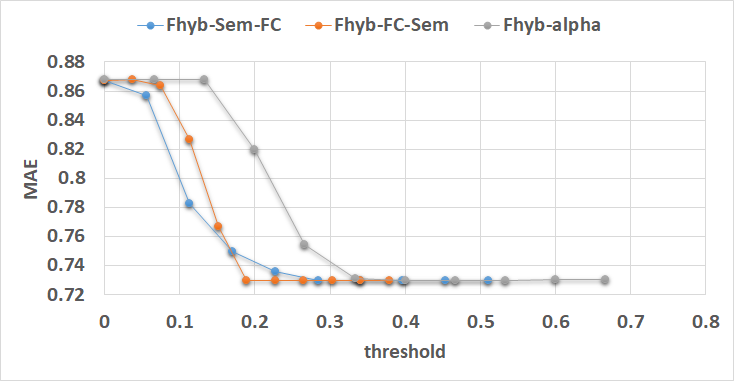
\includegraphics[width=0.9\textwidth]{hybsansclass.PNG}
	\caption{Évaluation MAE de l'hybridation sans classification des algorithmes FC et FSem}
	\label{fig:hybsansclassMAE}
\end{figure}

\begin{figure}[H]
	\centering
	\includegraphics[width=0.9\textwidth]{hybsansclassRMSE.PNG}
	\caption{Évaluation RMSE de l'hybridation sans classification des algorithmes FC et FSem}
	\label{fig:hybsansclassRMSE}
\end{figure}

Le tableau suivant présente les meilleures valeurs d'Alpha :
\begin{table}[H]
	\centering
	\begin{tabular}{|l|l|}
		\hline
		threshold & Best Alpha for threshold \\ \hline
		0 & 1 \\ \hline
		0.066666667 & 1 \\ \hline
		0.133333333 & 1 \\ \hline
		0.2 & 8 \\ \hline
		0.266666667 & 8 \\ \hline
		0.333333333 & 8 \\ \hline
		0.4 & 7 \\ \hline
		0.466666667 & 5 \\ \hline
		0.533333333 & 5 \\ \hline
		0.6 & 5 \\ \hline
		0.666666667 & 5 \\ \hline
	\end{tabular}
\captionof{table}{Tableau des differents seuils combiné à Alpha du FHyb pondéré}
\end{table}

Le tableau suivant \ref{tab:hyb} décrit les trois meilleures valeurs obtenues pour chaque algorithme en termes de MAE et RMSE.
\begin{table}[H]
	\centering
	\begin{tabular}{|l|l|l|l|}
		\hline
		threshold & 0.189 & 0.151 & 0.113 \\ \hline
		MAE  (FHyb-FC-Sem) & 0.73 & 0.767 & 0.827 \\ \hline
		RMSE (FHyb-FC-Sem) & 1.003 & 1.046 & \textbf{1.101} \\ \hline\hline
		threshold & 0.284& 0.227 & 0.17 \\ \hline
		MAE  (FHyb-Sem-FC) & 0.73 & 0.736 & 0.75 \\ \hline
		RMSE (FHyb-Sem-FC) & \textbf{1.001} & 1.007 & 1.023 \\ \hline\hline
		threshold & 0.466 & 0.533 & 0.6 \\ \hline
		Alpha & 0.5 & 0.5 & 0.5 \\ \hline
		MAE  (FHyb-alpha) & \textbf{0.7295} & 0.73 & 0.7301 \\ \hline
		RMSE (FHyb-alpha) & 1.0014 & 1.0018 & 1.002 \\ \hline
	\end{tabular}
	\captionof{table}{Récapitulatif des trois meilleurs résultats (MAE et RMSE) pour le FHyb pondéré}
	\label{tab:hyb}
\end{table}


\subsubsection*{Discussion des résultats}
Nous pouvons déduire de ces résultats que les trois hybridations donnent des résultats approximativement proches avec comme meilleure valeur de MAE égale à 0.73 et RMSE égale à 1.
Cependant, le FHyb pondéré à donnée la meilleurs valeurs de MAE qui est égale à 0.729 avec la valeur Alpha égales à 5.

\subsubsection*{FHyb avec classification}
Pour cette approche, nous ferons varier la valeur du nombre de clusters K dans les algorithmes suivants:
\begin{itemize}
\item FHyb pondéré K-NN (FHyb-alpha).
\item FHyb pondéré K-medoids (FHyb-alpha-Kmedoids).
\item FHyb collaboratif basé sémantique K-NN (FHyb-FC-Sem-KNN).
\item FHyb collaboratif basé sémantique K-medoids (FHyb-FC-Sem-Kmedoids).
\item FHyb collaboratif basé sémantique K-medoids et BSO (FHyb-FC-Sem-Kmedoids-BSO).
\item FHyb sémantique basé collaboratif K-NN (FHyb-Sem-FC-KNN).
\item FHyb sémantique basé collaboratif K-medoids (FHyb-Sem-FC-Kmedoids).
\item FHyb sémantique basé collaboratif K-medoids et BSO (FHyb-Sem-FC-Kmedoids-BSO).
\item FHyb Multivues K-NN (FHyb-Multiview-KNN).
\end{itemize}
\begin{figure}[H]
	\centering
	\includegraphics[width=0.9\textwidth]{hybclassMAE.PNG}
	\caption{Évaluation MAE des algorithmes hybrides basés classification}
	\label{fig:hybclassMAE}
\end{figure}


\begin{figure}[H]
	\centering
	\includegraphics[width=0.9\textwidth]{hybclassRMSE.PNG}
	\caption{Évaluation RMSE des algorithmes hybrides basés classification}
	\label{fig:hybclassRMSE}
\end{figure}

Le tableau suivant décrit les trois meilleures valeurs obtenues pour chaque algorithme en termes de MAE et RMSE.
\begin{table}[H]
	\centering
	\begin{tabular}{|l|l|l|l|}
		\hline
		k & 27 & 25 & 30 \\ \hline
		MAE(FHyb-FC-Sem-KNN) & \textbf{0.7171} &  0.7181 & 0.7185 \\ \hline
		RMSE(FHyb-FC-Sem-KNN)& \textbf{0.9946} &  0.9967 & 0.9950 \\ \hline\hline
		k & 15 & 45 & 30 \\ \hline
		MAE(FHyb-Sem-FC-KNN) & 0.7256& 0.7261& 0.7272 \\ \hline
		RMSE(FHyb-Sem-FC-KNN) & 1.003 & 1.0015 & 1.0030 \\ \hline\hline
		k & 65 & 55 & 45 \\ \hline
		MAE(FHyb-FC-Sem-Kmedoids-BSO) & 0.73001 & 0.7302 & 0.73064 \\ \hline
		RMSE(FHyb-FC-Sem-Kmedoids-BSO) & 1.0029 & 1.0029 & 1.0013 \\ \hline\hline
		k & 10 & 15 & 20 \\ \hline
		MAE(FHyb-Sem-FC-Kmedoids-BSO) & 0.7289 & 0.7309 & 0.7302 \\ \hline
		RMSE(FHyb-Sem-FC-Kmedoids-BSO) & 1.001 & 1.0034 & 1.0025 \\ \hline\hline
		k & 65 & 55 & 45 \\ \hline
		MAE(multiview\_knn\_svd) & 0.7300 & 0.7302 & 0.7306\\ \hline
		RMSE(multiview\_knn\_svd) & 1.0009 & 1.0017 & 1.0015 \\ \hline\hline
		k & 15 & 80 & 20 \\ \hline
		MAE(FHyb-Multiview-KNN) & 0.7294 & 0.7298 & 0.730\\ \hline
		RMSE(FHyb-Multiview-KNN) & 0.9994& 1.0015 & 0.9990 \\ \hline\hline
		k & 25 & 15 & 20 \\ \hline
		MAE(FHyb-Sem-FC-Kmedoids) & 0.7323 & 0.7324& 0.733 \\ \hline
		RMSE(FHyb-Sem-FC-Kmedoids) & 1.005& 1.004 & 1.0065 \\ \hline\hline
		k & 140 & 120 & 135 \\ \hline
		alpha & 0.1 & 0.4 & 0.6 \\ \hline
		MAE(FHyb-alpha-KNN) & 0.7287 & 0.7289 & 0.7289 \\ \hline
		RMSE(FHyb-alpha-KNN)& 0.9991 & 0.9991 & 0.9994\\ \hline\hline
		k & 15 & 20 & 10 \\ \hline
		alpha & 0.1 & 0.2 & 0.3 \\ \hline
		MAE(FHyb-alpha-Kmedoids) & 0.7300& 0.731 & 0.7312 \\ \hline
		RMSE(FHyb-alpha-Kmedoids) & 1.0015 & 1.0039 & 1.0021 \\ \hline
	\end{tabular}
\captionof{table}{Récapitulatif des trois meilleurs résultats (MAE et RMSE) pour les differents FHyb avec classification}
\end{table}
\subsubsection*{Discussion des résultats}
\myparagraph{FHyb pondéré} Pour ce filtrage l'ajout du clustering n'a pas amélioré les performances de la prédiction, car le Fhyb pondéré donne comme meilleure résultat 0.729 pour MAE et 1.001 pour RMSE, après l'ajout du clustering, MAE est passée à 0.730 et RMSE est restée presque la même.
Cependant l'ajout de la classification K-NN, a amélioré les performances de MAE qui est devenu 0.7287 et de RMSE qui est passé à 0.99.
 
\myparagraph{FHyb sémantique basé collaboratif} Après avoir incorporer le clustering K-medoids à ce filtrage, nous constatons que les évaluations ne se sont pas améliorées, car sans clustering MAE été égale à 0.73 et RMSE à 1.00, après l'ajout du clustering MAE est passée à 0.732 et RMSE est restée la même, donc on suppose que le choix des medoids d'une façon optimisée peut montrer l'apport du clustering, après avoir ajouté l'optimisation BSO, RMSE n'a pas changé mais MAE s'est améliorée et est passée à 0.728, donc le clustering optimisé est efficace sur ce filtrage.
Après l'ajout de la classification avec K-NN à ce filtrage, nous remarquons que MAE s'est améliorée et est devenu égale à 0.725, pour RMSE pas de changement à noter, donc la classification pour ce filtrage améliore la qualité de MAE seulement.

\myparagraph{FHyb collaboratif basé sémantique}
Ce filtrage sans classification a donnée comme meilleur résultat pour MAE=0.73 et RMSE=1.00, après l'ajout du clustering, MAE c'est améliorée et est passé à 0.729 et RMSE à 0.999 mais l'ajout de l'optimisation ne semble pas améliorer les performances de ces deux évaluations car elles ont passée respectivement à 0.73 et 1.00. Cependant l'ajout de la classification semble être la meilleure option à choisir pour ce filtrage car elle a fait passé MAE à 0.717 et RMSE à 0.994, donc elle est plus efficace que le clustering et le clustering optimisé.

\myparagraph{FHyb Multivues K-NN}
Ce filtrage utilise que la classification K-NN pour hybrider les deux vue sémantique et collaboratif, nous pouvons constaté qu'il a donné une valeur de 0.73 pour MAE et une valeur de 1.00 pour RMSE, donc pour cette base de donnée cette approche ne semble pas meilleure que les filtrages hybrides standard proposé ou avec classification car nous avons eu des performances mieux que celle-ci. 
Nous supposons que cette approche serait meilleure testée sur un autre dataset, de ce fait par la suite nous allons testé cette approche sur un autre jeu de données.

\subsubsection*{Comparaison des résultats avec d'autre méthodes utilisée sur MovieLens}
Pour voir si nos résultats sont de bonne qualité, nous avons décidé de les comparés à des méthodes déjà utilisé sur le dataset MovieLens 100k, les résultats peuvent être consultés sur le site \cite{ref42}.
Le tableau suivant est un récapitulatif de nos meilleurs résultats pour chaque approches développées:

\begin{table}[H]
	\centering
	\begin{tabular}{|l|l|l|}
		\hline
		& MAE & RMSE \\ \hline
		FC standard & 0.73 & 1.001 \\ \hline
		FC basé k-medoids & 0.733 & 1.004 \\ \hline
		FC basé k-medoids et BSO & 0.728 & 1.001 \\ \hline
		FC basé K-NN & 0.73 & 1.001 \\ \hline
		FSem standard & 0.729 & 1.002 \\ \hline
		FSem k-medoids & 0.730 & 1.001 \\ \hline
		FSem k-medoids et BSO & 0.728 & 1.002 \\ \hline
		FSem K-NN & 0.729 & 1.000 \\ \hline
		FHyb pondéré & 0.729 & 1.001 \\ \hline
		FHyb pondéré k-medoids & 0.730 & 1.001 \\ \hline
		FHyb pondéré K-NN & 0.728 & 0.991 \\ \hline
		FHyb Sem basé FC & 0.73 & 1.001 \\ \hline
		FHyb Sem basé FC k-medoids & 0.732 & 1.005 \\ \hline
		FHyb Sem basé FC k-medoids et BSO & 0.728 & 1.001 \\ \hline
		FHyb Sem basé FC K-NN & 0.725 & 1.003 \\ \hline
		FHyb FC basé Sem & 0.730 & 1.003 \\ \hline
		FHyb FC basé Sem k-medoids & 0.729 & 0.999 \\ \hline
		FHyb FC basé Sem k-medoids et BSO & 0.730 & 1.002 \\ \hline
		FHyb FC basé Sem K-NN & \cellcolor[HTML]{67FD9A}0.717 & \cellcolor[HTML]{67FD9A}0.994 \\ \hline
		FHyb mutivues K-NN & 0.730 & 1.000 \\ \hline
	\end{tabular}
\captionof{table}{Récapitulatif des meilleurs résultats (MAE et RMSE) pour touts les filtrages conçus}
 \label{tab:movie}
\end{table}
Le tableau suivant montre les résultats obtenu à partir du site \cite{ref42}.
Les deux méthodes utilisés sont SVDplusplus qui est une amélioration de la méthode SVD et UserKNNPearson qui est un filtrage collaboratif avec la corrélation de Pearson comme distance entre utilisateur et une classification des voisins des ces derniers avec l'algorithme K-NN.
\begin{table}[H]
	\centering
	\begin{tabular}{|l|l|l|}
		\hline
		& MAE & RMSE \\ \hline
		UserKNNPearson & 0.728 & 0.929 \\ \hline
		SVDPlusPlus version 1& 0.718 & 0.913 \\ \hline
		SVDPlusPlus  version 2& \cellcolor[HTML]{67FD9A} 0.713 & \cellcolor[HTML]{67FD9A}0.90829	\\ \hline
	\end{tabular}
\captionof{table}{Les meilleurs résultats (MAE et RMSE) trouvrer à partir de \cite{ref42} pour le dataset MovieLens 100k}
 \label{tab:mymedia}
\end{table}
Nous pouvons conclure que nos résultats sont dans les normes comparé avec ceux déjà développé ou part avant, de plus nous nous rapprochons avec notre méthode FHyb FC basé Sem et K-NN du résultat de SVDPlusPlus version 2 du tableau .
Sachant que la méthode de SVDPlusPlus prend beaucoup de temps pour s'exécutée, il serait possible d'opter pour notre approche qui est FHyb FC basé Sem et K-NN, qui s'exécutera plus rapidement que SVDPlusPlus, de plus notre approche est simple à implémenter et donne des résultats proches de la méthode SVDPlusPlus.\\


%%%%%%%%%%%%%%%%%%%%%%%%%%%%%%%%%%%%%%%%%%%%%%%%%%%%%%%%%%%%%
\textbf{B) Evaluations avec RED}\\
Afin de confirmer les résultats obtenus de nos approches sur le dataset MovieLens, nous avons décidé de refaire les testes sur un autre dataset qui est RED.
Nous avons choisi de refaire les testes que sur les approches qui ont donné de bons résultats, car nous somme limé par le temps et la puissance de calcul de nos machines.
\subsubsection*{Évaluations}
Dans cette partie, nous réaliserons un ensemble de tests portant sur les performances de notre approche et nous comparerons nos résultats avec les résultats des approches existantes. \\

\begin{enumerate}[nosep,label=\textbf{\arabic*)}]
	%%  \setcounter{enumi}{4}
	\item \textbf{Filtrage collaboratif avec classification et classification optimisée}
\end{enumerate}\mbox{}\indent{} Dans cette phase d’expérimentations, nous allons évaluer la qualité de la recommandation lorsque celle-ci est basée sur un FC basé K-medoids, FC basé K-medoids et BSO et FC basé K-NN. Nous ferons des expérimentations par rapport à la corrélation de Pearson, étant donné que celle-ci reste l’une des plus connues et des plus utilisées, et comme prétraitement du dataset nous avons opté pour la méthode SVD vu son efficacité d'après les testes précédent.
\begin{figure}[H]
	\centering
	\includegraphics[width=\textwidth]{epFCMAE.PNG}
	\caption{Évaluation MAE du FC avec classification sur RED}
	\label{fig:epFCMAE}
\end{figure}

\begin{figure}[H]
	\centering
	\includegraphics[width=\textwidth]{epFCRMSE.PNG}
	\caption{Évaluation RMSE du FC avec classification sur RED}
	\label{fig:epFCRMSE}
\end{figure}
Le tableau suivant décrit les trois meilleures valeurs obtenues en termes de MAE et RMSE.
\begin{table}[H]
	\centering
	\begin{tabular}{|l|l|l|l|}
		\hline
		k & 5 & 17 & 11 \\ \hline
		MAE(FC-user-user-KNN) & 0.7744 & 0.779 & 0.7798 \\ \hline
		RMSE(FC-user-user-KNN) & 1.066& 1.0709 & 1.0712 \\ \hline\hline
		k & 17 & 36 & 64 \\ \hline
		MAE(FC-user-user-Kmedoids-BSO) & \textbf{0.7677} & 0.7697  & 0.7684 \\ \hline
		RMSE(FC-user-user-Kmedoids-BSO) &\textbf{1.060} & 1.0697  & 1.07534 \\ \hline\hline
		k & 19 & 23 & 48 \\ \hline
		MAE(FC-user-user-Kmedoids) & 0.7751& 0.7753 & 0.7785\\ \hline
		RMSE(FC-user-user-Kmedoids) & 1.0659 & 1.06989 & 1.0814 \\ \hline
	\end{tabular}
\captionof{table}{Récapitulatif des trois meilleurs résultats (MAE et RMSE) pour le FC avec classification du dataset RED}
\end{table}
\subsubsection*{Discussion des résultats}
D'après le tableau récapitulatif et les graphes ci-dessus, nous constatons que l'approche qui donne les meilleurs résultats est le FC basé K-medoids et BSO avec MAE égale à 0.767 et RMSE égale à 1.060, ce qui confirme l'apport de l'optimisation sur le clustering.\\


%%%%%%%%%%%%%%%%%%%EP SEM%%%%%%%%%%%%%%%%%%%%%%%%%%%%%%
\begin{enumerate}[nosep,label=\textbf{\arabic*)}]
	\setcounter{enumi}{1}
	\item \textbf{Filtrage sémantique  avec classification et classification optimisée}
\end{enumerate}\mbox{} \indent Dans cette partie, nous allons évalué la qualité de la recommandation lorsque celle-ci est basée sur un FSem basé K-medoids, FSem basé K-medoids et BSO et FSem basé K-NN.  Nous ferons des expérimentations en utilisant la formule de distance d'intérêt entre utilisateur, et la distance de Wu and Palmer entre les items car le dataset RED possède une représentation sous forme d'ontologie des items.
Le prétraitement des valeurs manquantes est effectué avec la méthode SVD.
\begin{figure}[H]
	\centering
	\includegraphics[width=\textwidth]{epsemMAE.PNG}
	\caption{Évaluation MAE du FSem avec classification sur RED}
	\label{fig:epsemMAE}
\end{figure}

\begin{figure}[H]
	\centering
	\includegraphics[width=\textwidth]{epsemRMSE.PNG}
	\caption{Évaluation RMSE du FSem avec classification sur RED}
	\label{fig:epsemRMSE}
\end{figure}
La tableau suivant décrit les trois meilleures valeurs en termes de MAE et RMSE.
\begin{table}[H]
	\centering
	\begin{tabular}{|l|l|l|l|}
		\hline
		k & 12 & 32 & 46 \\ \hline
		MAE(FSem-user-user-Kmedoids) & 0.7765& 0.7771 & 0.7779\\ \hline
		RMSE(FSem-user-user-Kmedoids) & 1.0753 & 1.0775 & 1.0823 \\ \hline\hline
		k & 8 & 7 & 6 \\ \hline
		MAE(FSem-user-user-KNN) & 0.7778 & 0.7812 & 0.7832 \\ \hline
		RMSE(FSem-user-user-KNN) & 1.0790 & 1.0806 & 1.0834 \\ \hline\hline
		k & 43 & 20 & 46 \\ \hline
		MAE(FSem-user-user-Kmedoids-BSO) & \textbf{0.7637} & 0.7664 & 0.7664 \\ \hline
		RMSE(FSem-user-user-Kmedoids-BSO) & \textbf{1.064} & 1.0681 & 1.0750 \\ \hline
	\end{tabular}
\captionof{table}{Récapitulatif des trois meilleurs résultats (MAE et RMSE) pour le FSem avec classification du dataset RED}
\end{table}
\subsubsection*{Discussion des résultats}
D'après le tableau récapitulatif et les graphes ci-dessus, nous constatons que l'approche qui donne les meilleurs résultats est le FSem basé K-medoids et BSO avec MAE égale à 0.763 et RMSE égale à 1.064, ce qui confirme l'apport de l'optimisation sur le clustering.\\


%%%%%%%%%%%%%%%%%EP HYB%%%%%%%%%%%%%%%%%%%%%%%%%%%%%%%%%%%
\begin{enumerate}[nosep,label=\textbf{\arabic*)}]
	  \setcounter{enumi}{2}
	\item \textbf{Filtrage hybride avec classification et classification optimisée}
\end{enumerate}\mbox{}\indent Dans cette partie, nous allons évalué la qualité de la recommandation lorsque celle-ci est basée sur un FHyb basé K-medoids, FHyb basé K-medoids et BSO et FHyb basé K-NN.  Nous ferons des expérimentations par rapport à la corrélation de Pearson, étant donné que celle-ci reste l’une des plus connues et des plus utilisées, et comme prétraitement du dataset nous avons opté pour la méthode SVD vu son efficacité d'après les testes précédent.

\begin{figure}[H]
	\centering
	\includegraphics[width=\textwidth]{ephybMAE.PNG}
	\caption{Évaluation MAE du filtrage hybride avec classification sur RED}
	\label{fig:ephybMAE}
\end{figure}


\begin{figure}[H]
	\centering
	\includegraphics[width=\textwidth]{ephybRMSE.PNG}
	\caption{Évaluation RMSE du filtrage hybride avec classification sur RED}
	\label{fig:ephybRMSE}
\end{figure}
Le tableau suivant décrit les trois meilleurs valeurs obtenues pour chaque algorithme en termes de MAE et RMSE.
\begin{table}[H]
	\centering
	\begin{tabular}{|l|l|l|l|}
		\hline
		k & 10 & 8 & 11 \\ \hline
		MAE(FHyb-FC-Sem-KNN) & 0.7791 & 0.7812 & 0.7818 \\ \hline
		RMSE(FHyb-FC-Sem-KNN) & 1.0728 & 1.07503 & 1.07846 \\ \hline\hline
		k & 9 & 7 & 8 \\ \hline
		MAE(FHyb-Multiview) & \textbf{0.7657}& 0.7744 & 0.7744 \\ \hline
		RMSE(FHyb-Multiview) & \textbf{1.0703}& 1.0781 & 1.0812\\ \hline\hline
		k & 34 & 10 & 6 \\ \hline
		MAE(FHyb-FC-Sem-Kmedoids) & 0.784 & 0.7852 & 0.7865 \\ \hline
		RMSE(FHyb-FC-Sem-Kmedoids) & 1.0850 & 1.0762 & 1.07503 \\ \hline\hline
		k & 38 & 13 & 17 \\ \hline
		MAE(FHyb-FC-Sem-Kmedoids-BSO) & 0.7798 & 0.78053 & 0.7812 \\ \hline
		RMSE(FHyb-FC-Sem-Kmedoids-BSO) & 1.0825 & 1.0765 & 1.0769 \\ \hline
	\end{tabular}
\captionof{table}{Récapitulatif des trois meilleurs résultats (MAE et RMSE) pour le FHyb avec classification du dataset RED}
\end{table}

\subsubsection*{Discussion des résultats}
D'après le tableau récapitulatif et les graphes ci-dessus, nous constatons que l'approche qui donne les meilleurs résultats dans le cas d'un filtrage hybride est le FHyb multivues K-NN avec MAE égale à 0.765 et RMSE égale à 1.070, c'est l'approche inspiré du travail de \cite{ref30}.

\subsubsection*{Comparaison des résultats avec d'autre méthodes utilisée sur RED}
Pour voir si nos résultats sont de bonne qualité et dans les normes, nous avons décidé de les comparés à des méthodes déjà utilisé sur le dataset RED, les résultats peuvent être consultés sur le site \cite{ref43}.
Le tableau suivant est un récapitulatif de nos meilleurs résultats pour chaque approches développées:

\begin{table}[H]
	\centering
	\begin{tabular}{|l|l|l|}
		\hline
		             & MAE & RMSE \\ \hline
		FC basé K-NN & 0.774 & 1.065 \\ \hline
		FC basé k-medoids & 0.775 & 1.065 \\ \hline
		FC basé k-medoids et BSO & 0.767 & 1.060 \\ \hline
		FSem basé K-NN & 0.778 & 1.079 \\ \hline
		FSem basé k-medoids & 0.776 & 1.075 \\ \hline
		FSem basé k-medoids et BSO & \cellcolor[HTML]{67FD9A}0.763 & \cellcolor[HTML]{67FD9A}1.064 \\ \hline
		FHyb collaboratif basé sémantique K-NN & 0.779 & 1.072 \\ \hline
		FHyb collaboratif basé sémantique  et k-medoids & 0.784 & 1.085 \\ \hline
		FHyb collaboratif basé sémantique et k-medoids-BSO & 0.779 & 1.082 \\ \hline
		FHyb multivues & 0.765 & 1.070 \\ \hline
	\end{tabular}
\captionof{table}{Récapitulatif des meilleurs résultats (MAE et RMSE) pour les differents filtrage conçu et testés sur RED}
\end{table}
Sur le site \cite{ref43}, le meilleur résultat de MAE est de 0.804, et 1.047 pour RMSE avec la méthode SVD. En comparant nos résultats avec celui du site, nous pouvons dire que nous avons amélioré nettement MAE avec notre approche qui est FSem basé K-medoids et BSO avec MAE égale à 0.763, pour RMSE il n'y a pas une grande différence entre notre approche et SVD. Par conséquent nous avons prouvé l'efficacité de notre méthode comparé aux méthodes déjà appliqué sur le dataset RED.

\section{Récapitulatif des différents résultats des évaluations}
Dans cette partie nous allons récapituler les différents résultats obtenus pour chaque filtrage réalisé, en termes  d'hybridation, de classification et de classification optimisée sur les deux dataset utilisés.
\begin{enumerate}[nosep,label=\textbf{\arabic*)}]
	%%\setcounter{enumi}{2}
	\item Filtrage collaboratif
\end{enumerate}\mbox{} \indent
Pour le filtrage collaboratif standard, le clustering optimisé avec l'algorithme K-medoids et BSO a amélioré les résultats du FC standard.
En utilisant la classification avec K-NN sur le FC standard, cela n'a pas apporté d'amélioration. Donc pour le FC le meilleur filtrage est le FC basé K-medoids et BSO, il a pu donner des résultats très proches à ceux des algorithmes déjà appliqués sur MovieLens, d'environ 0.015 de différence pour MAE et de 0.092 pour RMSE.\\

\begin{enumerate}[nosep,label=\textbf{\arabic*)}]
	\setcounter{enumi}{1}
	\item \ Filtrage sémantique
\end{enumerate}\mbox{} \indent
Le FSem standard n'a pas pu être amélioré ni par la classification avec K-NN et ni par le clustering optimisé. Mais ses résultats restent dans les normes comparé aux résultats données par d'autres méthodes appliquées sur le dataset MovieLens, avec MAE égale à 0.7297 et RMSE égale à 1.0012.
En appliquant le FSem basé K-medoids, le FSem basé K-medoids-BSO et le FSem basé K-NN sur le dataset RED, nous avons obtenus de très bons résultats comparé à ceux du site \cite{ref43}.\\

\begin{enumerate}[nosep,label=\textbf{\arabic*)}]
	\setcounter{enumi}{2}
	\item Filtrage hybride
\end{enumerate}\mbox{} \indent
L'approche que nous avons conçue et qui a donné les meilleures performances sur le dataset MovieLens est le FHyb collaboratif basé sémantique et K-NN, ce résultat et très proche des meilleurs performance existantes de ce dataset (voir les deux tableaux \ref{tab:mymedia} et \ref{tab:movie}).

\subsubsection*{Comparaison entre les résultats de MovieLens et RED}
En rajoutant la classification et classification optimisée aux trois types de filtrages et après les avoirs testés sur le dataset RED, nous avons obtenu de très bons résultat comparé a ceux du site \cite{ref43}, et nous pouvons ainsi conclure et dire qu'il y'a un apport lors de l'ajout de la classification et la classification optimisée aux  différent types de filtrage conçus, car cela nous a permis de nous rapprocher des meilleurs résultats déjà existants dans le cas du dataset MovieLens, et de surpasser les performances des algorithmes déjà existants en utilisant le dataset RED.
\section{Conclusion}
Dans ce chapitre que nous clôturons, nous avons pu tester différents algorithmes
de recommandation que nous avons réalisé sur les datasets MovieLens 100k et RED.
En effet, ces expérimentations nous ont permis de faire des comparaison entre les différents filtrages conçus, et de conclure en disant que les filtrages conçus se sont montrés très efficace sur le dataset RED. Nous avons pu nous rapprocher des résultats déjà existants sur le dataset MovieLens avec notre approche (FHyb collaboratif basé sémantique et K-NN) qui est simple et plus rapide que SVDPlusPlus.  

\newpage
\thispagestyle{empty}
\setcounter{table}{1}
\begin{appendices}
\section*{Évaluation de MovieLens}
\subsection*{Filtrage collaboratif}
\begin{center}\label{tab30}
	\begin{tabularx}{\textwidth}{|l|X|X|X|X|X|X|X|X|X|X|X|}
		\hline
		threshold & 0.0 & 0.1 & 0.2 & 0.3 & 0.4 & 0.5 & 0.6 & 0.7 & 0.799 & 0.899 & 1.0 \\ \hline
		mae & 0.804 & 0.808 & 0.829 & 1.032 & 2.492 & 2.981 & 2.921 & 2.921 & 2.921 & 2.921 & 2.921 \\ \hline
		rmse & 1.076 & 1.085 & 1.133 & 1.476 & 2.837 & 3.178 & 3.119 & 3.119 & 3.119 & 3.119 & 3.119 \\ \hline				
	\end{tabularx}	
	\captionof{table}{Résultats de MAE et RMSE pour l'algorithme de FC item-item} 
\end{center}

\begin{center}\label{tab31}
	\begin{tabularx}{\textwidth}{|l|X|X|X|X|X|X|X|X|X|X|X|}
		\hline
		threshold & 0.0 & 0.1 & 0.2 & 0.3 & 0.4 & 0.5 & 0.6 & 0.7 & 0.799 & 0.899 & 1.0 \\ \hline
		mae & 0.852 & 0.853 & 0.851 & 0.831 & 0.775 & 0.782 & 0.78 & 0.78 & 0.78 & 0.78 & 0.78 \\ \hline
		rmse & 1.169 & 1.169 & 1.167 & 1.146 & 1.064 & 1.07 & 1.066 & 1.066 & 1.066 & 1.066 & 1.066 \\ \hline
	\end{tabularx}	
	\captionof{table}{Résultats de MAE et RMSE pour l'algorithme de FC item-item-IA} 
\end{center}


\begin{center}\label{tab3}
	\begin{tabularx}{\textwidth}{|l|X|X|X|X|X|X|X|X|X|X|X|}
		\hline
		threshold & 0.0 & 0.052 & 0.105 & 0.158 & 0.211 & 0.264 & 0.317 & 0.369 & 0.422 & 0.475 & 0.528 \\ \hline
		mae & 0.923 & 0.923 & 0.93 & 0.94 & 0.942 & 0.959 & 0.967 & 0.974 & 0.973 & 0.974 & 0.974 \\ \hline
		rmse & 1.197 & 1.198 & 1.207 & 1.217 & 1.225 & 1.245 & 1.254 & 1.259 & 1.26 & 1.259 & 1.259 \\ \hline
	\end{tabularx}	
	\captionof{table}{Résultats de MAE et RMSE pour l'algorithme de FC item-item-SVD} 
\end{center}

\begin{center}\label{tab4}
	\begin{tabularx}{\textwidth}{|l|X|X|X|X|X|X|X|X|X|X|X|}
		\hline
		threshold & 0.0 & 0.043 & 0.086 & 0.129 & 0.172 & 0.215 & 0.258 & 0.301 & 0.345 & 0.388 & 0.431 \\ \hline
		mae & 0.804 & 0.803 & 0.802 & 0.8 & 0.798 & 0.793 & 0.796 & 0.798 & 0.797 & 0.797 & 0.797 \\ \hline
		rmse & 1.076 & 1.074 & 1.073 & 1.071 & 1.07 & 1.065 & 1.067 & 1.068 & 1.067 & 1.067 & 1.067 \\ \hline
	\end{tabularx}	
	\captionof{table}{Résultats de MAE et RMSE pour l'algorithme de FC item-item-UA} 
\end{center}

\begin{center}\label{tab5}
	\begin{tabularx}{\textwidth}{|l|X|X|X|X|X|X|X|X|X|X|X|}
		\hline
		threshold & 0.0 & 0.075 & 0.151 & 0.227 & 0.303 & 0.378 & 0.454 & 0.53 & 0.606 & 0.681 & 0.757 \\ \hline
		mae & 0.795 & 0.795 & 0.795 & 0.81 & 1.022 & 1.957 & 2.612 & 2.941 & 2.948 & 2.948 & 2.948 \\ \hline
		rmse & 1.079 & 1.079 & 1.079 & 1.111 & 1.492 & 2.504 & 2.842 & 3.135 & 3.143 & 3.142 & 3.142 \\ \hline
	\end{tabularx}	
	\captionof{table}{Résultats de MAE et RMSE pour l'algorithme de FC user-user} 
\end{center}



\begin{center}\label{tab6}
	\begin{tabularx}{\textwidth}{|l|X|X|X|X|X|X|X|X|X|X|X|}
		\hline
		threshold & 0.0 & 0.036 & 0.073 & 0.109 & 0.146 & 0.183 & 0.219 & 0.256 & 0.292 & 0.329 & 0.366 \\ \hline
		mae & 1.028 & 0.821 & 0.798 & 0.799 & 0.801 & 0.801 & 0.801 & 0.8 & 0.8 & 0.8 & 0.8 \\ \hline
		rmse & 1.265 & 1.093 & 1.069 & 1.07 & 1.071 & 1.072 & 1.072 & 1.07 & 1.07 & 1.07 & 1.07 \\ \hline
	\end{tabularx}	
	\captionof{table}{Résultats de MAE et RMSE pour l'algorithme de FC user-user-IA} 
\end{center}


\begin{center}\label{tab7}
	\begin{tabularx}{\textwidth}{|l|X|X|X|X|X|X|X|X|X|X|X|}
		\hline
		threshold & 0 & 0.075 & 0.151 & 0.227 & 0.303 & 0.378 & 0.454 & 0.53 & 0.606 & 0.681 & 0.757 \\ \hline
		mae & 0.795 & 0.795 & 0.795 & 0.795 & 0.796 & 0.795 & 0.761 & 0.781 & 0.78 & 0.78 & 0.78 \\ \hline
		rmse & 1.079 & 1.079 & 1.079 & 1.079 & 1.081 & 1.08 & 1.047 & 1.066 & 1.066 & 1.066 & 1.066 \\ \hline
	\end{tabularx}	
	\captionof{table}{Résultats de MAE et RMSE pour l'algorithme de FC user-user-UA} 
\end{center}

\begin{center}\label{tab8}
	\begin{tabularx}{\textwidth}{|l|X|X|X|X|X|X|X|X|X|X|}	
		\hline
		threshold & 0.0 & 0.056 & 0.113 & 0.17 & 0.227 & 0.284 & 0.34 & 0.397 & 0.454 & 0.511 \\ \hline
		mae & 0.867 & 0.857 & 0.783 & 0.75 & 0.736 & 0.73 & 0.73 & 0.73 & 0.73 & 0.73 \\ \hline
		rmse & 1.129 & 1.12 & 1.056 & 1.023 & 1.007 & 1.001 & 1.001 & 1.002 & 1.002 & 1.002 \\ \hline
	\end{tabularx}	
	\captionof{table}{Résultats de MAE et RMSE pour l'algorithme de FC user-user-SVD} 
\end{center}


\begin{center} \label{tab9}
	\begin{tabularx}{\textwidth}{|l|X|X|X|X|X|X|X|X|X|X|X|X|} 
		\hline 
		K & 10 & 15 & 20 & 25 & 30 & 35 & 40 & 45 & 50 & 55 & 60 & 65 \\ \hline 
		mae & 0.733 & 0.732 & 0.735 & 0.735 & 0.736 & 0.732 & 0.736 & 0.734 & 0.736 & 0.74 & 0.737 & 0.74 \\ \hline 
		rmse & 1.004 & 1.003 & 1.006 & 1.006 & 1.008 & 1.005 & 1.008 & 1.007 & 1.008 & 1.011 & 1.011 & 1.012 \\ \hline 
		\hline 
		K & 70 & 75 & 80 & 85 & 90 & 95 & 100 & 105 & 110 & 115 & 120 & 125 \\ \hline 
		mae & 0.743 & 0.737 & 0.739 & 0.738 & 0.744 & 0.747 & 0.745 & 0.746 & 0.747 & 0.74 & 0.751 & 0.747 \\ \hline 
		rmse & 1.015 & 1.011 & 1.011 & 1.011 & 1.015 & 1.02 & 1.017 & 1.017 & 1.02 & 1.015 & 1.024 & 1.019 \\ \hline 
		\hline 
		K & 130 & 135 & 140 & 145 & 150 & 155 & 160 & 165 & 170 & 175 & 180 & 185 \\ \hline 
		mae & 0.753 & 0.744 & 0.756 & 0.747 & 0.752 & 0.755 & 0.746 & 0.745 & 0.76 & 0.754 & 0.753 & 0.759 \\ \hline 
		rmse & 1.025 & 1.019 & 1.028 & 1.021 & 1.027 & 1.028 & 1.021 & 1.021 & 1.036 & 1.026 & 1.027 & 1.033 \\ \hline 
		\hline 
		K & 190 & 195 & 200 & 205 & 210 & 215 & 220 & 225 & 230 & 235 & 240 & 245 \\ \hline 
		mae & 0.754 & 0.761 & 0.76 & 0.752 & 0.76 & 0.755 & 0.755 & 0.76 & 0.766 & 0.76 & 0.76 & 0.762 \\ \hline 
		rmse & 1.028 & 1.033 & 1.037 & 1.026 & 1.034 & 1.027 & 1.03 & 1.03 & 1.038 & 1.039 & 1.032 & 1.036 \\ \hline 
		\hline 
		K & 250 & 255 & 260 & 265 & 270 & 275 & 280 & 285 & 290 & 295 & 300 & 305 \\ \hline 
		mae & 0.764 & 0.769 & 0.763 & 0.754 & 0.766 & 0.77 & 0.771 & 0.776 & 0.766 & 0.764 & 0.766 & 0.775 \\ \hline 
		rmse & 1.037 & 1.042 & 1.042 & 1.03 & 1.04 & 1.039 & 1.044 & 1.053 & 1.041 & 1.039 & 1.043 & 1.051 \\ \hline 
		\hline 
		K & 310 & 315 & 320 & 325 & 330 & 335 & 340 & 345 & 350 & 355 & 360 & 365 \\ \hline 
		mae & 0.766 & 0.774 & 0.768 & 0.778 & 0.775 & 0.77 & 0.767 & 0.776 & 0.772 & 0.78 & 0.777 & 0.78 \\ \hline 
		rmse & 1.041 & 1.048 & 1.048 & 1.049 & 1.052 & 1.043 & 1.041 & 1.053 & 1.047 & 1.056 & 1.052 & 1.056 \\ \hline 
		\hline 
		K & 370 & 375 & 380 & 385 & 390 & 395 & 400 & 405 & 410 & 415 & 420 & 425 \\ \hline 
		mae & 0.778 & 0.78 & 0.774 & 0.778 & 0.778 & 0.782 & 0.781 & 0.786 & 0.779 & 0.78 & 0.777 & 0.79 \\ \hline 
		rmse & 1.051 & 1.052 & 1.052 & 1.053 & 1.058 & 1.051 & 1.052 & 1.059 & 1.054 & 1.054 & 1.051 & 1.067 \\ \hline 
		\hline 
		K & 430 & 435 & 440 & 445 & 450 & 455 & 460 & 465 & 470 & 475 & 480 & 485 \\ \hline 
		mae & 0.785 & 0.786 & 0.784 & 0.786 & 0.787 & 0.791 & 0.784 & 0.792 & 0.784 & 0.792 & 0.79 & 0.79 \\ \hline 
		rmse & 1.063 & 1.063 & 1.057 & 1.058 & 1.056 & 1.06 & 1.057 & 1.064 & 1.06 & 1.069 & 1.066 & 1.062 \\ \hline 
		\hline 
		K & 490 & 495 & 500 & 505 & 510 & 515 & 520 & 525 & 530 & 535 & 540 & 545 \\ \hline 
		mae & 0.797 & 0.788 & 0.789 & 0.791 & 0.795 & 0.798 & 0.794 & 0.808 & 0.792 & 0.79 & 0.808 & 0.791 \\ \hline 
		rmse & 1.07 & 1.061 & 1.066 & 1.063 & 1.067 & 1.072 & 1.062 & 1.076 & 1.069 & 1.064 & 1.081 & 1.06 \\ \hline 
		\hline 
		K & 550 & 555 & 560 & 565 & 570 & 575 & 580 & 585 & 590 & 595 & 600 & 605 \\ \hline 
		mae & 0.797 & 0.792 & 0.806 & 0.795 & 0.8 & 0.818 & 0.798 & 0.8 & 0.79 & 0.793 & 0.799 & 0.805 \\ \hline 
		rmse & 1.074 & 1.067 & 1.078 & 1.068 & 1.07 & 1.094 & 1.07 & 1.073 & 1.06 & 1.064 & 1.074 & 1.079 \\ \hline 
		\hline 
		K & 610 & 615 & 620 & 625 & 630 & 635 & 640 & 645 & 650 & 655 & 660 & 665 \\ \hline 
		mae & 0.811 & 0.798 & 0.811 & 0.811 & 0.807 & 0.806 & 0.798 & 0.812 & 0.807 & 0.807 & 0.812 & 0.811 \\ \hline 
		rmse & 1.08 & 1.066 & 1.081 & 1.089 & 1.079 & 1.078 & 1.07 & 1.083 & 1.084 & 1.081 & 1.081 & 1.085 \\ \hline 
		\hline 
		K & 670 & 675 & 680 & 685 & 690 & 695  & & & & & & \\ \hline 
		mae & 0.811 & 0.823 & 0.816 & 0.808 & 0.806 & 0.816 & & & & & &  \\ \hline 
		rmse & 1.081 & 1.091 & 1.09 & 1.076 & 1.086 & 1.087  & & & & & & \\ \hline 
	\end{tabularx} 
	\captionof{table}{Résultats de MAE et RMSE pour l'algorithme de FC user-user-Kmedoids} 
\end{center}

\begin{center} \label{tab10}
	\begin{tabularx}{\textwidth}{|l|X|X|X|X|X|X|X|X|X|X|X|X|} 
		\hline 
		K & 10 & 15 & 20 & 25 & 30 & 35 & 40 & 45 & 50 & 55 & 60 & 65 \\ \hline 
		mae & 0.733 & 0.733 & 0.732 & 0.733 & 0.732 & 0.732 & 0.731 & 0.73 & 0.73 & 0.73 & 0.731 & 0.73 \\ \hline 
		rmse & 1.002 & 1.003 & 1.002 & 1.004 & 1.002 & 1.003 & 1.001 & 1.001 & 1.001 & 1.001 & 1.001 & 1 \\ \hline 
		\hline 
		K & 70 & 75 & 80 & 85 & 90 & 95 & 100 & 105 & 110 & 115 & 120 & 125 \\ \hline 
		mae & 0.731 & 0.731 & 0.731 & 0.73 & 0.731 & 0.731 & 0.73 & 0.731 & 0.73 & 0.73 & 0.728 & 0.729 \\ \hline 
		rmse & 1 & 1.001 & 1.001 & 1.001 & 1.001 & 1.001 & 1.001 & 1.001 & 1.001 & 1 & 0.999 & 0.999 \\ \hline 
		\hline 
		K & 130 & 135 & 140 & 145 & 150 & 155 & 160 & 165 & 170 & 175 & 180 & 185 \\ \hline 
		mae & 0.729 & 0.728 & 0.729 & 0.729 & 0.73 & 0.73 & 0.73 & 0.73 & 0.73 & 0.73 & 0.73 & 0.73 \\ \hline 
		rmse & 0.999 & 0.999 & 0.999 & 1 & 1 & 1 & 1.001 & 1 & 1 & 1.001 & 1.001 & 1.001 \\ \hline 
		\hline 
		K & 190 & 195 & 200 & 205 & 210 & 215 & 220 & 225 & 230 & 235 & 240 & 245 \\ \hline 
		mae & 0.73 & 0.73 & 0.731 & 0.73 & 0.731 & 0.73 & 0.73 & 0.731 & 0.731 & 0.73 & 0.73 & 0.731 \\ \hline 
		rmse & 1 & 1.001 & 1.001 & 1.001 & 1.001 & 1.001 & 1.001 & 1.001 & 1.001 & 1.001 & 1.001 & 1.001 \\ \hline 
		\hline 
		K & 250 & 255 & 260 & 265 & 270 & 275 & 280 & 285 & 290 & 295 & 300 & 305 \\ \hline 
		mae & 0.73 & 0.73 & 0.73 & 0.73 & 0.73 & 0.73 & 0.73 & 0.73 & 0.73 & 0.73 & 0.729 & 0.73 \\ \hline 
		rmse & 1.001 & 1.001 & 1.001 & 1.001 & 1.001 & 1.001 & 1.001 & 1.001 & 1.001 & 1.001 & 1.001 & 1.001 \\ \hline 
		\hline 
		K & 310 & 315 & 320 & 325 & 330 & 335 & 340 & 345 & 350 & 355 & 360 & 365 \\ \hline 
		mae & 0.73 & 0.729 & 0.73 & 0.729 & 0.729 & 0.729 & 0.729 & 0.729 & 0.729 & 0.729 & 0.729 & 0.729 \\ \hline 
		rmse & 1.001 & 1.001 & 1.001 & 1.001 & 1.001 & 1.001 & 1 & 1 & 1.001 & 1 & 1 & 1.001 \\ \hline 
		\hline 
		K & 370 & 375 & 380 & 385 & 390 & 395 & 400 & 405 & 410 & 415 & 420 & 425 \\ \hline 
		mae & 0.729 & 0.729 & 0.73 & 0.73 & 0.73 & 0.73 & 0.729 & 0.729 & 0.729 & 0.729 & 0.729 & 0.729 \\ \hline 
		rmse & 1 & 1.001 & 1.001 & 1.001 & 1.001 & 1.001 & 1.001 & 1 & 1 & 1.001 & 1 & 1.001 \\ \hline 
		\hline 
		K & 430 & 435 & 440 & 445 & 450 & 455 & 460 & 465 & 470 & 475 & 480 & 485 \\ \hline 
		mae & 0.729 & 0.729 & 0.729 & 0.73 & 0.73 & 0.729 & 0.73 & 0.729 & 0.729 & 0.729 & 0.729 & 0.729 \\ \hline 
		rmse & 1.001 & 1 & 1.001 & 1.001 & 1.001 & 1.001 & 1.001 & 1 & 1 & 1 & 1 & 1 \\ \hline 
		\hline 
		K & 490 & 495 & 500 & 505 & 510 & 515 & 520 & 525 & 530 & 535 & 540 & 545 \\ \hline 
		mae & 0.73 & 0.729 & 0.729 & 0.729 & 0.729 & 0.729 & 0.729 & 0.73 & 0.729 & 0.729 & 0.729 & 0.729 \\ \hline 
		rmse & 1 & 1 & 1 & 1 & 1 & 1 & 1 & 1 & 1 & 1 & 0.999 & 0.999 \\ \hline 
		\hline 
		K & 550 & 555 & 560 & 565 & 570 & 575 & 580 & 585 & 590 & 595 & 600 & 605 \\ \hline 
		mae & 0.729 & 0.73 & 0.73 & 0.73 & 0.73 & 0.73 & 0.729 & 0.729 & 0.729 & 0.729 & 0.729 & 0.73 \\ \hline 
		rmse & 1 & 1.001 & 1.001 & 1.001 & 1.001 & 1.001 & 1.001 & 1 & 1 & 1.001 & 1.001 & 1.001 \\ \hline 
		\hline 
		K & 610 & 615 & 620 & 625 & 630 & 635 & 640 & 645 & 650 & 655 & 660 & 665 \\ \hline 
		mae & 0.73 & 0.73 & 0.73 & 0.73 & 0.73 & 0.731 & 0.731 & 0.73 & 0.73 & 0.73 & 0.73 & 0.73 \\ \hline 
		rmse & 1.001 & 1.001 & 1.001 & 1.001 & 1.001 & 1.002 & 1.002 & 1.001 & 1.002 & 1.001 & 1.001 & 1.001 \\ \hline 
		\hline 
		K & 670 & 675 & 680 & 685 & 690 & 695  & & & & & & \\ \hline 
		mae & 0.73 & 0.729 & 0.73 & 0.729 & 0.729 & 0.73 & & & & & &  \\ \hline 
		rmse & 1.001 & 1.001 & 1.001 & 1.001 & 1.001 & 1.001  & & & & & & \\ \hline 
	\end{tabularx} 
	\captionof{table}{Résultats de MAE et RMSE pour l'algorithme de FC user-user-KNN}  
\end{center}

\subsection*{Filtrage sémantique}
\begin{center}\label{tab21}
	\begin{tabularx}{\textwidth}{|l|X|X|X|X|X|X|X|X|X|X|X|}
		\hline
		threshold & 0.666 & 0.666 & 0.666 & 0.666 & 0.666 & 0.666 & 0.666 & 0.666 & 0.666 & 0.666 & 0.666 \\ \hline
		mae & 0.867 & 0.867 & 0.811 & 0.736 & 0.729 & 0.73 & 0.73 & 0.73 & 0.73 & 0.73 & 0.73 \\ \hline
		rmse & 1.129 & 1.128 & 1.085 & 1.009 & 1.001 & 1.002 & 1.002 & 1.002 & 1.002 & 1.002 & 1.002 \\ \hline
	\end{tabularx}	
	\captionof{table}{Résultats de MAE et RMSE pour l'algorithme de FSem user-user} 
\end{center}

\begin{center} \label{tab22}	
	\begin{tabularx}{\textwidth}{|l|X|X|X|X|X|X|X|X|X|X|X|X|} 
		\hline 
		K & 10 & 15 & 20 & 25 & 30 & 35 & 40 & 45 & 50 & 55 & 60 & 65 \\ \hline 
		mae & 0.73 & 0.73 & 0.732 & 0.73 & 0.734 & 0.733 & 0.735 & 0.735 & 0.737 & 0.737 & 0.736 & 0.737 \\ \hline 
		rmse & 1.002 & 1.001 & 1.005 & 1.002 & 1.005 & 1.004 & 1.007 & 1.007 & 1.006 & 1.008 & 1.006 & 1.008 \\ \hline 
		\hline 
		K & 70 & 75 & 80 & 85 & 90 & 95 & 100 & 105 & 110 & 115 & 120 & 125 \\ \hline 
		mae & 0.739 & 0.737 & 0.738 & 0.739 & 0.739 & 0.745 & 0.748 & 0.745 & 0.747 & 0.746 & 0.744 & 0.747 \\ \hline 
		rmse & 1.011 & 1.009 & 1.01 & 1.011 & 1.011 & 1.017 & 1.016 & 1.018 & 1.017 & 1.018 & 1.015 & 1.018 \\ \hline 
		\hline 
		K & 130 & 135 & 140 & 145 & 150 & 155 & 160 & 165 & 170 & 175 & 180 & 185 \\ \hline 
		mae & 0.743 & 0.751 & 0.752 & 0.749 & 0.751 & 0.753 & 0.755 & 0.752 & 0.757 & 0.753 & 0.758 & 0.763 \\ \hline 
		rmse & 1.014 & 1.022 & 1.024 & 1.019 & 1.023 & 1.026 & 1.024 & 1.024 & 1.028 & 1.026 & 1.027 & 1.034 \\ \hline 
		\hline 
		K & 190 & 195 & 200 & 205 & 210 & 215 & 220 & 225 & 230 & 235 & 240 & 245 \\ \hline 
		mae & 0.753 & 0.753 & 0.757 & 0.765 & 0.764 & 0.754 & 0.759 & 0.759 & 0.76 & 0.769 & 0.752 & 0.776 \\ \hline 
		rmse & 1.024 & 1.023 & 1.028 & 1.037 & 1.034 & 1.026 & 1.029 & 1.03 & 1.034 & 1.041 & 1.025 & 1.044 \\ \hline 
		\hline 
		K & 250 & 255 & 260 & 265 & 270 & 275 & 280 & 285 & 290 & 295 & 300 & 305 \\ \hline 
		mae & 0.761 & 0.77 & 0.772 & 0.77 & 0.763 & 0.768 & 0.762 & 0.765 & 0.771 & 0.771 & 0.768 & 0.773 \\ \hline 
		rmse & 1.03 & 1.04 & 1.044 & 1.039 & 1.033 & 1.035 & 1.032 & 1.036 & 1.043 & 1.042 & 1.04 & 1.044 \\ \hline 
		\hline 
		K & 310 & 315 & 320 & 325 & 330 & 335 & 340 & 345 & 350 & 355 & 360 & 365 \\ \hline 
		mae & 0.771 & 0.775 & 0.768 & 0.778 & 0.77 & 0.778 & 0.774 & 0.775 & 0.78 & 0.788 & 0.781 & 0.776 \\ \hline 
		rmse & 1.043 & 1.049 & 1.037 & 1.049 & 1.041 & 1.051 & 1.044 & 1.042 & 1.051 & 1.058 & 1.051 & 1.043 \\ \hline 
		\hline 
		K & 370 & 375 & 380 & 385 & 390 & 395 & 400 & 405 & 410 & 415 & 420 & 425 \\ \hline 
		mae & 0.778 & 0.78 & 0.783 & 0.79 & 0.783 & 0.783 & 0.78 & 0.784 & 0.779 & 0.78 & 0.788 & 0.796 \\ \hline 
		rmse & 1.045 & 1.051 & 1.052 & 1.06 & 1.056 & 1.051 & 1.05 & 1.052 & 1.048 & 1.049 & 1.055 & 1.063 \\ \hline 
		\hline 
		K & 430 & 435 & 440 & 445 & 450 & 455 & 460 & 465 & 470 & 475 & 480 & 485 \\ \hline 
		mae & 0.786 & 0.797 & 0.788 & 0.779 & 0.795 & 0.796 & 0.789 & 0.786 & 0.784 & 0.788 & 0.801 & 0.792 \\ \hline 
		rmse & 1.057 & 1.069 & 1.059 & 1.047 & 1.062 & 1.07 & 1.059 & 1.057 & 1.056 & 1.059 & 1.073 & 1.06 \\ \hline 
		\hline 
		K & 490 & 495 & 500 & 505 & 510 & 515 & 520 & 525 & 530 & 535 & 540 & 545 \\ \hline 
		mae & 0.791 & 0.801 & 0.797 & 0.794 & 0.793 & 0.81 & 0.794 & 0.803 & 0.802 & 0.796 & 0.807 & 0.798 \\ \hline 
		rmse & 1.064 & 1.069 & 1.063 & 1.059 & 1.061 & 1.078 & 1.066 & 1.072 & 1.066 & 1.066 & 1.076 & 1.066 \\ \hline 
		\hline 
		K & 550 & 555 & 560 & 565 & 570 & 575 & 580 & 585 & 590 & 595 & 600 & 605 \\ \hline 
		mae & 0.81 & 0.795 & 0.798 & 0.806 & 0.805 & 0.795 & 0.8 & 0.798 & 0.809 & 0.807 & 0.808 & 0.806 \\ \hline 
		rmse & 1.079 & 1.063 & 1.062 & 1.073 & 1.071 & 1.068 & 1.069 & 1.067 & 1.076 & 1.073 & 1.078 & 1.076 \\ \hline 
		\hline 
		K & 610 & 615 & 620 & 625 & 630 & 635 & 640 & 645 & 650 & 655 & 660 & 665 \\ \hline 
		mae & 0.818 & 0.803 & 0.805 & 0.807 & 0.8 & 0.818 & 0.816 & 0.805 & 0.809 & 0.805 & 0.812 & 0.812 \\ \hline 
		rmse & 1.085 & 1.073 & 1.074 & 1.074 & 1.069 & 1.085 & 1.08 & 1.074 & 1.076 & 1.072 & 1.084 & 1.077 \\ \hline 
		\hline 
		K & 670 & 675 & 680 & 685 & 690 & 695  & & & & & & \\ \hline 
		mae & 0.81 & 0.81 & 0.809 & 0.812 & 0.815 & 0.81 & & & & & &  \\ \hline 
		rmse & 1.075 & 1.076 & 1.081 & 1.08 & 1.081 & 1.078  & & & & & & \\ \hline 
	\end{tabularx} 
	\captionof{table}{Résultats de MAE et RMSE pour l'algorithme de FSem user-user-Kmedoids}
\end{center}
\subsection*{Filtrage hybride}

\begin{center}\label{tab11}
	\begin{tabularx}{\textwidth}{|l|X|X|X|X|X|X|X|X|X|X|X|}\hline
		threshold & 0 & 0.066 & 0.133 & 0.2 & 0.266 & 0.333 & 0.4 & 0.466 & 0.533 & 0.6 & 0.666 \\ \hline
		alpha & 1 & 1 & 1 & 8 & 8 & 8 & 7 & 5 & 5 & 5 & 5 \\ \hline
		mae & 0.867 & 0.867 & 0.867 & 0.819 & 0.754 & 0.73 & 0.73 & 0.729 & 0.73 & 0.73 & 0.73 \\ \hline
		rmse & 1.129 & 1.129 & 1.129 & 1.088 & 1.027 & 1.002 & 1.001 & 1.001 & 1.001 & 1.002 & 1.002 \\ \hline
	\end{tabularx}	
	\captionof{table}{Résultats de MAE et RMSE pour l'algorithme de FHyb-alpha}
\end{center}

\begin{center} \label{tab12}
	\begin{tabularx}{\textwidth}{|l|X|X|X|X|X|X|X|X|X|X|X|X|} 
		\hline 
		K & 10 & 15 & 20 & 25 & 30 & 35 & 40 & 45 & 50 & 55 & 60 & 65 \\ \hline 
		mae & 3 & 1 & 2 & 1 & 6 & 6 & 1 & 1 & 7 & 1 & 2 & 1 \\ \hline 
		rmse & 0.731 & 0.73 & 0.731 & 0.732 & 0.731 & 0.736 & 0.734 & 0.731 & 0.734 & 0.74 & 0.738 & 0.74 \\ \hline 
		\hline 
		K & 70 & 75 & 80 & 85 & 90 & 95 & 100 & 105 & 110 & 115 & 120 & 125 \\ \hline 
		mae & 1 & 8 & 7 & 6 & 8 & 3 & 6 & 1 & 4 & 1 & 1 & 4 \\ \hline 
		rmse & 0.741 & 0.743 & 0.739 & 0.742 & 0.743 & 0.743 & 0.746 & 0.742 & 0.742 & 0.747 & 0.747 & 0.749 \\ \hline 
		\hline 
		K & 130 & 135 & 140 & 145 & 150 & 155 & 160 & 165 & 170 & 175 & 180 & 185 \\ \hline 
		mae & 3 & 3 & 5 & 3 & 2 & 8 & 1 & 3 & 5 & 8 & 8 & 3 \\ \hline 
		rmse & 0.749 & 0.747 & 0.742 & 0.753 & 0.75 & 0.745 & 0.747 & 0.75 & 0.758 & 0.748 & 0.752 & 0.752 \\ \hline 
		\hline 
		K & 190 & 195 & 200 & 205 & 210 & 215 & 220 & 225 & 230 & 235 & 240 & 245 \\ \hline 
		mae & 8 & 3 & 3 & 3 & 2 & 3 & 8 & 1 & 3 & 1 & 1 & 3 \\ \hline 
		rmse & 0.758 & 0.761 & 0.757 & 0.75 & 0.762 & 0.757 & 0.759 & 0.76 & 0.758 & 0.764 & 0.77 & 0.764 \\ \hline 
		\hline 
		K & 250 & 255 & 260 & 265 & 270 & 275 & 280 & 285 & 290 & 295 & 300 & 305 \\ \hline 
		mae & 8 & 5 & 6 & 5 & 1 & 1 & 2 & 5 & 5 & 8 & 1 & 7 \\ \hline 
		rmse & 0.765 & 0.767 & 0.766 & 0.761 & 0.766 & 0.769 & 0.771 & 0.763 & 0.765 & 0.77 & 0.763 & 0.774 \\ \hline 
		\hline 
		K & 310 & 315 & 320 & 325 & 330 & 335 & 340 & 345 & 350 & 355 & 360 & 365 \\ \hline 
		mae & 2 & 4 & 5 & 7 & 2 & 1 & 1 & 8 & 6 & 6 & 4 & 3 \\ \hline 
		rmse & 0.768 & 0.765 & 0.776 & 0.767 & 0.766 & 0.772 & 0.773 & 0.777 & 0.772 & 0.784 & 0.778 & 0.779 \\ \hline 
		\hline 
		K & 370 & 375 & 380 & 385 & 390 & 395 & 400 & 405 & 410 & 415 & 420 & 425 \\ \hline 
		mae & 6 & 1 & 8 & 4 & 3 & 8 & 1 & 2 & 4 & 7 & 1 & 3 \\ \hline 
		rmse & 0.777 & 0.78 & 0.785 & 0.781 & 0.772 & 0.78 & 0.789 & 0.782 & 0.786 & 0.778 & 0.787 & 0.785 \\ \hline 
		\hline 
		K & 430 & 435 & 440 & 445 & 450 & 455 & 460 & 465 & 470 & 475 & 480 & 485 \\ \hline 
		mae & 3 & 2 & 8 & 1 & 1 & 8 & 6 & 2 & 6 & 1 & 7 & 3 \\ \hline 
		rmse & 0.776 & 0.78 & 0.788 & 0.793 & 0.786 & 0.793 & 0.788 & 0.799 & 0.794 & 0.792 & 0.789 & 0.79 \\ \hline 
		\hline 
		K & 490 & 495 & 500 & 505 & 510 & 515 & 520 & 525 & 530 & 535 & 540 & 545 \\ \hline 
		mae & 3 & 3 & 7 & 1 & 1 & 1 & 1 & 1 & 6 & 2 & 4 & 3 \\ \hline 
		rmse & 0.792 & 0.792 & 0.796 & 0.79 & 0.787 & 0.797 & 0.792 & 0.799 & 0.789 & 0.796 & 0.794 & 0.791 \\ \hline 
		\hline 
		K & 550 & 555 & 560 & 565 & 570 & 575 & 580 & 585 & 590 & 595 & 600 & 605 \\ \hline 
		mae & 3 & 2 & 1 & 1 & 3 & 2 & 4 & 1 & 3 & 3 & 6 & 3 \\ \hline 
		rmse & 0.812 & 0.794 & 0.802 & 0.799 & 0.793 & 0.8 & 0.801 & 0.808 & 0.803 & 0.8 & 0.8 & 0.796 \\ \hline 
		\hline 
		K & 610 & 615 & 620 & 625 & 630 & 635 & 640 & 645 & 650 & 655 & 660 & 665 \\ \hline 
		mae & 7 & 1 & 8 & 8 & 7 & 3 & 2 & 3 & 3 & 1 & 7 & 7 \\ \hline 
		rmse & 0.816 & 0.8 & 0.806 & 0.8 & 0.809 & 0.806 & 0.813 & 0.813 & 0.804 & 0.811 & 0.803 & 0.805 \\ \hline 
		\hline 
		K & 670 & 675 & 680 & 685 & 690 & 695  & & & & & & \\ \hline 
		mae & 3 & 1 & 8 & 1 & 2 & 1 & & & & & &  \\ \hline 
		rmse & 0.805 & 0.807 & 0.812 & 0.804 & 0.817 & 0.814  & & & & & & \\ \hline 
	\end{tabularx} 
	\captionof{table}{Résultats de MAE et RMSE pour l'algorithme de FHyb alpha-Kmedoids}
\end{center}
\begin{center} \label{tab13}
	\begin{tabularx}{\textwidth}{|l|X|X|X|X|X|X|X|X|X|X|X|X|} 
		\hline 
		K & 10 & 15 & 20 & 25 & 30 & 35 & 40 & 45 & 50 & 55 & 60 & 65 \\ \hline 
		mae & 1 & 3 & 1 & 8 & 1 & 1 & 7 & 7 & 1 & 6 & 6 & 8 \\ \hline 
		rmse & 0.733 & 0.734 & 0.732 & 0.732 & 0.732 & 0.732 & 0.731 & 0.73 & 0.73 & 0.73 & 0.731 & 0.73 \\ \hline 
		\hline 
		K & 70 & 75 & 80 & 85 & 90 & 95 & 100 & 105 & 110 & 115 & 120 & 125 \\ \hline 
		mae & 2 & 1 & 3 & 1 & 5 & 8 & 4 & 1 & 4 & 1 & 4 & 1 \\ \hline 
		rmse & 0.731 & 0.731 & 0.731 & 0.73 & 0.731 & 0.731 & 0.731 & 0.73 & 0.73 & 0.729 & 0.728 & 0.73 \\ \hline 
		\hline 
		K & 130 & 135 & 140 & 145 & 150 & 155 & 160 & 165 & 170 & 175 & 180 & 185 \\ \hline 
		mae & 1 & 6 & 1 & 1 & 1 & 8 & 8 & 5 & 1 & 8 & 7 & 6 \\ \hline 
		rmse & 0.729 & 0.728 & 0.728 & 0.729 & 0.729 & 0.73 & 0.73 & 0.73 & 0.73 & 0.73 & 0.73 & 0.73 \\ \hline 
		\hline 
		K & 190 & 195 & 200 & 205 & 210 & 215 & 220 & 225 & 230 & 235 & 240 & 245 \\ \hline 
		mae & 1 & 1 & 1 & 1 & 8 & 1 & 1 & 1 & 2 & 6 & 1 & 1 \\ \hline 
		rmse & 0.73 & 0.73 & 0.73 & 0.73 & 0.73 & 0.73 & 0.73 & 0.73 & 0.73 & 0.73 & 0.73 & 0.73 \\ \hline 
		\hline 
		K & 250 & 255 & 260 & 265 & 270 & 275 & 280 & 285 & 290 & 295 & 300 & 305 \\ \hline 
		mae & 1 & 7 & 8 & 1 & 3 & 3 & 1 & 1 & 1 & 1 & 5 & 6 \\ \hline 
		rmse & 0.73 & 0.73 & 0.73 & 0.73 & 0.73 & 0.73 & 0.73 & 0.729 & 0.729 & 0.73 & 0.729 & 0.73 \\ \hline 
		\hline 
		K & 310 & 315 & 320 & 325 & 330 & 335 & 340 & 345 & 350 & 355 & 360 & 365 \\ \hline 
		mae & 8 & 1 & 8 & 1 & 1 & 1 & 6 & 4 & 7 & 6 & 7 & 8 \\ \hline 
		rmse & 0.73 & 0.729 & 0.729 & 0.729 & 0.729 & 0.729 & 0.729 & 0.729 & 0.73 & 0.729 & 0.729 & 0.729 \\ \hline 
		\hline 
		K & 370 & 375 & 380 & 385 & 390 & 395 & 400 & 405 & 410 & 415 & 420 & 425 \\ \hline 
		mae & 8 & 3 & 1 & 1 & 7 & 1 & 1 & 8 & 1 & 1 & 8 & 2 \\ \hline 
		rmse & 0.729 & 0.729 & 0.729 & 0.729 & 0.73 & 0.73 & 0.729 & 0.729 & 0.729 & 0.729 & 0.729 & 0.729 \\ \hline 
		\hline 
		K & 430 & 435 & 440 & 445 & 450 & 455 & 460 & 465 & 470 & 475 & 480 & 485 \\ \hline 
		mae & 1 & 8 & 8 & 1 & 1 & 1 & 5 & 1 & 1 & 3 & 7 & 6 \\ \hline 
		rmse & 0.729 & 0.729 & 0.729 & 0.729 & 0.729 & 0.729 & 0.729 & 0.73 & 0.729 & 0.729 & 0.729 & 0.73 \\ \hline 
		\hline 
		K & 490 & 495 & 500 & 505 & 510 & 515 & 520 & 525 & 530 & 535 & 540 & 545 \\ \hline 
		mae & 1 & 1 & 4 & 8 & 5 & 1 & 6 & 1 & 1 & 6 & 8 & 8 \\ \hline 
		rmse & 0.73 & 0.73 & 0.729 & 0.729 & 0.73 & 0.729 & 0.729 & 0.729 & 0.729 & 0.729 & 0.729 & 0.729 \\ \hline 
		\hline 
		K & 550 & 555 & 560 & 565 & 570 & 575 & 580 & 585 & 590 & 595 & 600 & 605 \\ \hline 
		mae & 6 & 6 & 1 & 1 & 6 & 4 & 1 & 1 & 1 & 5 & 1 & 6 \\ \hline 
		rmse & 0.73 & 0.73 & 0.73 & 0.73 & 0.73 & 0.729 & 0.729 & 0.729 & 0.729 & 0.729 & 0.729 & 0.73 \\ \hline 
		\hline 
		K & 610 & 615 & 620 & 625 & 630 & 635 & 640 & 645 & 650 & 655 & 660 & 665 \\ \hline 
		mae & 1 & 1 & 3 & 1 & 8 & 2 & 2 & 1 & 7 & 1 & 6 & 4 \\ \hline 
		rmse & 0.729 & 0.73 & 0.73 & 0.73 & 0.73 & 0.73 & 0.73 & 0.73 & 0.73 & 0.73 & 0.729 & 0.729 \\ \hline 
		\hline 
		K & 670 & 675 & 680 & 685 & 690 & 695  & & & & & & \\ \hline 
		mae & 1 & 1 & 4 & 8 & 2 & 1 & & & & & &  \\ \hline 
		rmse & 0.73 & 0.73 & 0.73 & 0.729 & 0.729 & 0.729  & & & & & & \\ \hline 
	\end{tabularx} 
	\captionof{table}{Résultats de MAE et RMSE pour l'algorithme de FHyb alpha-KNN} 
\end{center}

\begin{center}\label{tab14}
	\begin{tabularx}{\textwidth}{|l|X|X|X|X|X|X|X|X|X|X|X|}
		\hline
		threshold & 0 & 0.037 & 0.075 & 0.113 & 0.151 & 0.189 & 0.227 & 0.265 & 0.303 & 0.341 & 0.379 \\ \hline
		mae & 0.867 & 0.868 & 0.864 & 0.827 & 0.767 & 0.73 & 0.73 & 0.73 & 0.73 & 0.73 & 0.73 \\ \hline
		rmse & 1.129 & 1.13 & 1.127 & 1.101 & 1.046 & 1.003 & 1.003 & 1.002 & 1.002 & 1.002 & 1.002 \\ \hline
	\end{tabularx}	
	\captionof{table}{Résultats de MAE et RMSE pour l'algorithme de FHyb FC basé Sem}
\end{center}
\begin{center} \label{tab15}
	\begin{tabularx}{\textwidth}{|l|X|X|X|X|X|X|X|X|X|X|X|X|} 
		\hline 
		K & 10 & 15 & 20 & 25 & 30 & 35 & 40 & 45 & 50 & 55 & 60 & 65 \\ \hline 
		mae & 0.73 & 0.729 & 0.73 & 0.732 & 0.731 & 0.731 & 0.732 & 0.733 & 0.733 & 0.732 & 0.731 & 0.733 \\ \hline 
		rmse & 1.001 & 0.999 & 0.999 & 1.004 & 1.002 & 1.004 & 1.003 & 1.004 & 1.004 & 1.001 & 1.004 & 1.003 \\ \hline 
		\hline 
		K & 70 & 75 & 80 & 85 & 90 & 95 & 100 & 105 & 110 & 115 & 120 & 125 \\ \hline 
		mae & 0.733 & 0.735 & 0.729 & 0.74 & 0.736 & 0.736 & 0.735 & 0.741 & 0.741 & 0.741 & 0.737 & 0.741 \\ \hline 
		rmse & 1.006 & 1.007 & 1.001 & 1.011 & 1.007 & 1.008 & 1.009 & 1.016 & 1.014 & 1.016 & 1.012 & 1.011 \\ \hline 
		\hline 
		K & 130 & 135 & 140 & 145 & 150 & 155 & 160 & 165 & 170 & 175 & 180 & 185 \\ \hline 
		mae & 0.744 & 0.739 & 0.745 & 0.746 & 0.741 & 0.748 & 0.742 & 0.75 & 0.747 & 0.742 & 0.746 & 0.745 \\ \hline 
		rmse & 1.014 & 1.011 & 1.016 & 1.018 & 1.012 & 1.021 & 1.018 & 1.021 & 1.019 & 1.019 & 1.018 & 1.022 \\ \hline 
		\hline 
		K & 190 & 195 & 200 & 205 & 210 & 215 & 220 & 225 & 230 & 235 & 240 & 245 \\ \hline 
		mae & 0.746 & 0.75 & 0.75 & 0.747 & 0.747 & 0.761 & 0.747 & 0.759 & 0.75 & 0.749 & 0.753 & 0.761 \\ \hline 
		rmse & 1.019 & 1.026 & 1.025 & 1.023 & 1.025 & 1.033 & 1.024 & 1.03 & 1.026 & 1.026 & 1.027 & 1.036 \\ \hline 
		\hline 
		K & 250 & 255 & 260 & 265 & 270 & 275 & 280 & 285 & 290 & 295 & 300 & 305 \\ \hline 
		mae & 0.756 & 0.766 & 0.761 & 0.753 & 0.764 & 0.757 & 0.776 & 0.765 & 0.756 & 0.76 & 0.762 & 0.766 \\ \hline 
		rmse & 1.031 & 1.04 & 1.036 & 1.027 & 1.036 & 1.035 & 1.05 & 1.038 & 1.031 & 1.035 & 1.036 & 1.043 \\ \hline 
		\hline 
		K & 310 & 315 & 320 & 325 & 330 & 335 & 340 & 345 & 350 & 355 & 360 & 365 \\ \hline 
		mae & 0.764 & 0.766 & 0.761 & 0.775 & 0.767 & 0.775 & 0.767 & 0.773 & 0.774 & 0.768 & 0.772 & 0.777 \\ \hline 
		rmse & 1.038 & 1.042 & 1.038 & 1.051 & 1.04 & 1.048 & 1.046 & 1.052 & 1.051 & 1.041 & 1.048 & 1.053 \\ \hline 
		\hline 
		K & 370 & 375 & 380 & 385 & 390 & 395 & 400 & 405 & 410 & 415 & 420 & 425 \\ \hline 
		mae & 0.777 & 0.777 & 0.767 & 0.771 & 0.781 & 0.787 & 0.776 & 0.778 & 0.776 & 0.769 & 0.78 & 0.778 \\ \hline 
		rmse & 1.049 & 1.055 & 1.045 & 1.047 & 1.054 & 1.06 & 1.05 & 1.051 & 1.053 & 1.046 & 1.059 & 1.053 \\ \hline 
		\hline 
		K & 430 & 435 & 440 & 445 & 450 & 455 & 460 & 465 & 470 & 475 & 480 & 485 \\ \hline 
		mae & 0.781 & 0.78 & 0.778 & 0.784 & 0.783 & 0.779 & 0.793 & 0.791 & 0.795 & 0.785 & 0.79 & 0.79 \\ \hline 
		rmse & 1.059 & 1.06 & 1.054 & 1.063 & 1.056 & 1.053 & 1.068 & 1.069 & 1.067 & 1.063 & 1.064 & 1.067 \\ \hline 
		\hline 
		K & 490 & 495 & 500 & 505 & 510 & 515 & 520 & 525 & 530 & 535 & 540 & 545 \\ \hline 
		mae & 0.791 & 0.79 & 0.794 & 0.786 & 0.793 & 0.809 & 0.797 & 0.799 & 0.79 & 0.794 & 0.795 & 0.795 \\ \hline 
		rmse & 1.065 & 1.068 & 1.065 & 1.062 & 1.067 & 1.087 & 1.07 & 1.075 & 1.068 & 1.069 & 1.07 & 1.068 \\ \hline 
		\hline 
		K & 550 & 555 & 560 & 565 & 570 & 575 & 580 & 585 & 590 & 595 & 600 & 605 \\ \hline 
		mae & 0.798 & 0.798 & 0.785 & 0.801 & 0.788 & 0.791 & 0.797 & 0.79 & 0.801 & 0.806 & 0.797 & 0.797 \\ \hline 
		rmse & 1.077 & 1.073 & 1.058 & 1.079 & 1.066 & 1.069 & 1.067 & 1.064 & 1.076 & 1.08 & 1.076 & 1.073 \\ \hline 
		\hline 
		K & 610 & 615 & 620 & 625 & 630 & 635 & 640 & 645 & 650 & 655 & 660 & 665 \\ \hline 
		mae & 0.808 & 0.805 & 0.803 & 0.803 & 0.816 & 0.806 & 0.798 & 0.812 & 0.805 & 0.801 & 0.804 & 0.803 \\ \hline 
		rmse & 1.082 & 1.079 & 1.076 & 1.078 & 1.089 & 1.079 & 1.08 & 1.084 & 1.088 & 1.075 & 1.082 & 1.074 \\ \hline 
		\hline 
		K & 670 & 675 & 680 & 685 & 690 & 695  & & & & & & \\ \hline 
		mae & 0.813 & 0.806 & 0.807 & 0.811 & 0.799 & 0.817 & & & & & &  \\ \hline 
		rmse & 1.089 & 1.077 & 1.081 & 1.082 & 1.079 & 1.091  & & & & & & \\ \hline 
	\end{tabularx} 
	\captionof{table}{Résultats de MAE et RMSE pour l'algorithme de FHyb FC basé Sem et Kmedoids}
\end{center}

\begin{center} \label{tab16}
	\begin{tabularx}{\textwidth}{|l|X|X|X|X|X|X|X|X|X|X|X|X|} 
		\hline 
		K & 10 & 15 & 20 & 25 & 30 & 35 & 40 & 45 & 50 & 55 & 60 & 65 \\ \hline 
		mae & 0.728 & 0.723 & 0.72 & 0.718 & 0.718 & 0.722 & 0.719 & 0.72 & 0.721 & 0.722 & 0.721 & 0.723 \\ \hline 
		rmse & 1.007 & 1.002 & 0.996 & 0.996 & 0.995 & 0.997 & 0.996 & 0.995 & 0.995 & 0.994 & 0.995 & 0.996 \\ \hline 
		\hline 
		K & 70 & 75 & 80 & 85 & 90 & 95 & 100 & 105 & 110 & 115 & 120 & 125 \\ \hline 
		mae & 0.722 & 0.722 & 0.721 & 0.723 & 0.723 & 0.724 & 0.723 & 0.724 & 0.725 & 0.723 & 0.725 & 0.725 \\ \hline 
		rmse & 0.995 & 0.996 & 0.995 & 0.996 & 0.996 & 0.996 & 0.995 & 0.997 & 0.997 & 0.996 & 0.997 & 0.998 \\ \hline 
		\hline 
		K & 130 & 135 & 140 & 145 & 150 & 155 & 160 & 165 & 170 & 175 & 180 & 185 \\ \hline 
		mae & 0.725 & 0.725 & 0.725 & 0.726 & 0.724 & 0.724 & 0.724 & 0.724 & 0.724 & 0.724 & 0.724 & 0.723 \\ \hline 
		rmse & 0.998 & 0.997 & 0.997 & 0.998 & 0.997 & 0.997 & 0.997 & 0.997 & 0.997 & 0.997 & 0.996 & 0.996 \\ \hline 
		\hline 
		K & 190 & 195 & 200 & 205 & 210 & 215 & 220 & 225 & 230 & 235 & 240 & 245 \\ \hline 
		mae & 0.724 & 0.723 & 0.723 & 0.723 & 0.723 & 0.723 & 0.722 & 0.723 & 0.723 & 0.723 & 0.723 & 0.723 \\ \hline 
		rmse & 0.997 & 0.996 & 0.995 & 0.996 & 0.996 & 0.996 & 0.996 & 0.996 & 0.996 & 0.996 & 0.997 & 0.996 \\ \hline 
		\hline 
		K & 250 & 255 & 260 & 265 & 270 & 275 & 280 & 285 & 290 & 295 & 300 & 305 \\ \hline 
		mae & 0.723 & 0.724 & 0.725 & 0.725 & 0.725 & 0.725 & 0.725 & 0.724 & 0.725 & 0.725 & 0.726 & 0.726 \\ \hline 
		rmse & 0.996 & 0.997 & 0.998 & 0.997 & 0.997 & 0.998 & 0.998 & 0.997 & 0.998 & 0.998 & 0.998 & 0.999 \\ \hline 
		\hline 
		K & 310 & 315 & 320 & 325 & 330 & 335 & 340 & 345 & 350 & 355 & 360 & 365 \\ \hline 
		mae & 0.726 & 0.727 & 0.727 & 0.727 & 0.727 & 0.728 & 0.728 & 0.727 & 0.728 & 0.727 & 0.728 & 0.727 \\ \hline 
		rmse & 0.999 & 1 & 0.999 & 0.999 & 0.999 & 1 & 1 & 0.999 & 1 & 1 & 1 & 1 \\ \hline 
		\hline 
		K & 370 & 375 & 380 & 385 & 390 & 395 & 400 & 405 & 410 & 415 & 420 & 425 \\ \hline 
		mae & 0.727 & 0.728 & 0.728 & 0.727 & 0.727 & 0.728 & 0.727 & 0.728 & 0.728 & 0.727 & 0.727 & 0.727 \\ \hline 
		rmse & 1 & 1 & 1 & 1 & 1 & 1 & 1 & 1 & 1 & 1 & 1 & 1 \\ \hline 
		\hline 
		K & 430 & 435 & 440 & 445 & 450 & 455 & 460 & 465 & 470 & 475 & 480 & 485 \\ \hline 
		mae & 0.727 & 0.728 & 0.728 & 0.729 & 0.729 & 0.728 & 0.728 & 0.728 & 0.729 & 0.729 & 0.729 & 0.729 \\ \hline 
		rmse & 1 & 1 & 1 & 1.001 & 1.002 & 1.001 & 1.001 & 1.001 & 1.002 & 1.001 & 1.001 & 1.001 \\ \hline 
		\hline 
		K & 490 & 495 & 500 & 505 & 510 & 515 & 520 & 525 & 530 & 535 & 540 & 545 \\ \hline 
		mae & 0.729 & 0.73 & 0.73 & 0.73 & 0.729 & 0.73 & 0.73 & 0.73 & 0.73 & 0.729 & 0.729 & 0.729 \\ \hline 
		rmse & 1.001 & 1.002 & 1.002 & 1.002 & 1.002 & 1.002 & 1.002 & 1.002 & 1.002 & 1.002 & 1.002 & 1.002 \\ \hline 
		\hline 
		K & 550 & 555 & 560 & 565 & 570 & 575 & 580 & 585 & 590 & 595 & 600 & 605 \\ \hline 
		mae & 0.73 & 0.729 & 0.73 & 0.73 & 0.73 & 0.729 & 0.73 & 0.729 & 0.73 & 0.73 & 0.729 & 0.729 \\ \hline 
		rmse & 1.002 & 1.002 & 1.002 & 1.002 & 1.002 & 1.002 & 1.002 & 1.002 & 1.002 & 1.002 & 1.002 & 1.002 \\ \hline 
		\hline 
		K & 610 & 615 & 620 & 625 & 630 & 635 & 640 & 645 & 650 & 655 & 660 & 665 \\ \hline 
		mae & 0.729 & 0.729 & 0.729 & 0.729 & 0.729 & 0.729 & 0.729 & 0.729 & 0.729 & 0.729 & 0.73 & 0.73 \\ \hline 
		rmse & 1.002 & 1.001 & 1.002 & 1.002 & 1.002 & 1.002 & 1.001 & 1.002 & 1.002 & 1.002 & 1.002 & 1.002 \\ \hline 
		\hline 
		K & 670 & 675 & 680 & 685 & 690 & 695  & & & & & & \\ \hline 
		mae & 0.729 & 0.729 & 0.729 & 0.729 & 0.729 & 0.729 & & & & & &  \\ \hline 
		rmse & 1.002 & 1.002 & 1.002 & 1.002 & 1.001 & 1.002  & & & & & & \\ \hline 
	\end{tabularx} 
	\captionof{table}{Résultats de MAE et RMSE pour l'algorithme de FHyb FC basé Sem et K-NN}
\end{center}

\begin{center}\label{tab17}
	\begin{tabularx}{\textwidth}{|l|X|X|X|X|X|X|X|X|X|X|}
		\hline
		threshold & 0 & 0.056 & 0.113 & 0.17 & 0.227 & 0.284 & 0.34 & 0.397 & 0.454 & 0.511 \\ \hline
		mae & 0.867 & 0.857 & 0.783 & 0.75 & 0.736 & 0.73 & 0.73 & 0.73 & 0.73 & 0.73 \\ \hline
		rmse & 1.129 & 1.12 & 1.056 & 1.023 & 1.007 & 1.001 & 1.001 & 1.002 & 1.002 & 1.002 \\ \hline
	\end{tabularx}	
	\captionof{table}{Résultats de MAE et RMSE pour l'algorithme de FHyb Sem basé FC}
\end{center}



\begin{center} \label{tab18}
	\begin{tabularx}{\textwidth}{|l|X|X|X|X|X|X|X|X|X|X|X|X|} 
		\hline 
		K & 10 & 15 & 20 & 25 & 30 & 35 & 40 & 45 & 50 & 55 & 60 & 65 \\ \hline 
		mae & 0.733 & 0.732 & 0.733 & 0.732 & 0.733 & 0.736 & 0.735 & 0.734 & 0.736 & 0.739 & 0.74 & 0.746 \\ \hline 
		rmse & 1.004 & 1.004 & 1.006 & 1.005 & 1.006 & 1.008 & 1.008 & 1.008 & 1.009 & 1.014 & 1.013 & 1.015 \\ \hline 
		\hline 
		K & 70 & 75 & 80 & 85 & 90 & 95 & 100 & 105 & 110 & 115 & 120 & 125 \\ \hline 
		mae & 0.737 & 0.742 & 0.741 & 0.739 & 0.742 & 0.741 & 0.743 & 0.749 & 0.749 & 0.745 & 0.745 & 0.745 \\ \hline 
		rmse & 1.01 & 1.015 & 1.015 & 1.014 & 1.018 & 1.013 & 1.016 & 1.023 & 1.021 & 1.021 & 1.015 & 1.019 \\ \hline 
		\hline 
		K & 130 & 135 & 140 & 145 & 150 & 155 & 160 & 165 & 170 & 175 & 180 & 185 \\ \hline 
		mae & 0.748 & 0.745 & 0.749 & 0.746 & 0.752 & 0.753 & 0.749 & 0.758 & 0.756 & 0.756 & 0.755 & 0.754 \\ \hline 
		rmse & 1.02 & 1.019 & 1.022 & 1.022 & 1.027 & 1.024 & 1.024 & 1.032 & 1.034 & 1.032 & 1.028 & 1.032 \\ \hline 
		\hline 
		K & 190 & 195 & 200 & 205 & 210 & 215 & 220 & 225 & 230 & 235 & 240 & 245 \\ \hline 
		mae & 0.759 & 0.761 & 0.754 & 0.763 & 0.753 & 0.761 & 0.759 & 0.756 & 0.761 & 0.761 & 0.768 & 0.761 \\ \hline 
		rmse & 1.033 & 1.035 & 1.028 & 1.039 & 1.028 & 1.033 & 1.035 & 1.032 & 1.034 & 1.038 & 1.046 & 1.037 \\ \hline 
		\hline 
		K & 250 & 255 & 260 & 265 & 270 & 275 & 280 & 285 & 290 & 295 & 300 & 305 \\ \hline 
		mae & 0.767 & 0.763 & 0.758 & 0.761 & 0.771 & 0.768 & 0.767 & 0.768 & 0.773 & 0.771 & 0.775 & 0.772 \\ \hline 
		rmse & 1.045 & 1.038 & 1.035 & 1.033 & 1.044 & 1.042 & 1.042 & 1.037 & 1.044 & 1.044 & 1.049 & 1.043 \\ \hline 
		\hline 
		K & 310 & 315 & 320 & 325 & 330 & 335 & 340 & 345 & 350 & 355 & 360 & 365 \\ \hline 
		mae & 0.778 & 0.769 & 0.77 & 0.772 & 0.781 & 0.776 & 0.775 & 0.776 & 0.776 & 0.774 & 0.777 & 0.779 \\ \hline 
		rmse & 1.049 & 1.046 & 1.04 & 1.041 & 1.054 & 1.051 & 1.047 & 1.053 & 1.051 & 1.047 & 1.052 & 1.053 \\ \hline 
		\hline 
		K & 370 & 375 & 380 & 385 & 390 & 395 & 400 & 405 & 410 & 415 & 420 & 425 \\ \hline 
		mae & 0.787 & 0.784 & 0.784 & 0.781 & 0.782 & 0.781 & 0.778 & 0.787 & 0.787 & 0.784 & 0.8 & 0.778 \\ \hline 
		rmse & 1.06 & 1.058 & 1.052 & 1.054 & 1.056 & 1.053 & 1.053 & 1.06 & 1.064 & 1.059 & 1.072 & 1.052 \\ \hline 
		\hline 
		K & 430 & 435 & 440 & 445 & 450 & 455 & 460 & 465 & 470 & 475 & 480 & 485 \\ \hline 
		mae & 0.774 & 0.788 & 0.789 & 0.789 & 0.791 & 0.797 & 0.793 & 0.797 & 0.788 & 0.787 & 0.792 & 0.794 \\ \hline 
		rmse & 1.051 & 1.06 & 1.066 & 1.062 & 1.065 & 1.069 & 1.066 & 1.068 & 1.058 & 1.062 & 1.067 & 1.068 \\ \hline 
		\hline 
		K & 490 & 495 & 500 & 505 & 510 & 515 & 520 & 525 & 530 & 535 & 540 & 545 \\ \hline 
		mae & 0.791 & 0.792 & 0.807 & 0.805 & 0.796 & 0.797 & 0.793 & 0.806 & 0.8 & 0.794 & 0.798 & 0.802 \\ \hline 
		rmse & 1.062 & 1.063 & 1.08 & 1.08 & 1.069 & 1.071 & 1.066 & 1.079 & 1.073 & 1.064 & 1.07 & 1.075 \\ \hline 
		\hline 
		K & 550 & 555 & 560 & 565 & 570 & 575 & 580 & 585 & 590 & 595 & 600 & 605 \\ \hline 
		mae & 0.797 & 0.794 & 0.811 & 0.8 & 0.798 & 0.796 & 0.803 & 0.812 & 0.792 & 0.801 & 0.805 & 0.808 \\ \hline 
		rmse & 1.069 & 1.067 & 1.082 & 1.073 & 1.072 & 1.073 & 1.073 & 1.083 & 1.062 & 1.07 & 1.077 & 1.081 \\ \hline 
		\hline 
		K & 610 & 615 & 620 & 625 & 630 & 635 & 640 & 645 & 650 & 655 & 660 & 665 \\ \hline 
		mae & 0.81 & 0.803 & 0.798 & 0.807 & 0.814 & 0.8 & 0.797 & 0.812 & 0.802 & 0.804 & 0.816 & 0.813 \\ \hline 
		rmse & 1.076 & 1.078 & 1.071 & 1.081 & 1.088 & 1.072 & 1.069 & 1.087 & 1.074 & 1.075 & 1.09 & 1.084 \\ \hline 
		\hline 
		K & 670 & 675 & 680 & 685 & 690 & 695  & & & & & & \\ \hline 
		mae & 0.818 & 0.818 & 0.812 & 0.818 & 0.82 & 0.822 & & & & & &  \\ \hline 
		rmse & 1.089 & 1.086 & 1.085 & 1.091 & 1.089 & 1.093  & & & & & & \\ \hline 
	\end{tabularx} 
	\captionof{table}{Résultats de MAE et RMSE pour l'algorithme de FHyb Sem basé FC et K-medoids}
\end{center}

\begin{center} \label{tab19}
	\begin{tabularx}{\textwidth}{|l|X|X|X|X|X|X|X|X|X|X|X|X|} 
		\hline 
		K & 10 & 15 & 20 & 25 & 30 & 35 & 40 & 45 & 50 & 55 & 60 & 65 \\ \hline 
		mae & 0.733 & 0.733 & 0.732 & 0.733 & 0.732 & 0.732 & 0.731 & 0.73 & 0.73 & 0.73 & 0.731 & 0.73 \\ \hline 
		rmse & 1.002 & 1.003 & 1.002 & 1.004 & 1.002 & 1.003 & 1.001 & 1.001 & 1.001 & 1.001 & 1.001 & 1 \\ \hline 
		\hline 
		K & 70 & 75 & 80 & 85 & 90 & 95 & 100 & 105 & 110 & 115 & 120 & 125 \\ \hline 
		mae & 0.731 & 0.731 & 0.731 & 0.73 & 0.731 & 0.731 & 0.73 & 0.731 & 0.73 & 0.73 & 0.728 & 0.729 \\ \hline 
		rmse & 1 & 1.001 & 1.001 & 1.001 & 1.001 & 1.001 & 1.001 & 1.001 & 1.001 & 1 & 0.999 & 0.999 \\ \hline 
		\hline 
		K & 130 & 135 & 140 & 145 & 150 & 155 & 160 & 165 & 170 & 175 & 180 & 185 \\ \hline 
		mae & 0.729 & 0.728 & 0.729 & 0.729 & 0.73 & 0.73 & 0.73 & 0.73 & 0.73 & 0.73 & 0.73 & 0.73 \\ \hline 
		rmse & 0.999 & 0.999 & 0.999 & 1 & 1 & 1 & 1.001 & 1 & 1 & 1.001 & 1.001 & 1.001 \\ \hline 
		\hline 
		K & 190 & 195 & 200 & 205 & 210 & 215 & 220 & 225 & 230 & 235 & 240 & 245 \\ \hline 
		mae & 0.73 & 0.73 & 0.731 & 0.73 & 0.731 & 0.73 & 0.73 & 0.731 & 0.731 & 0.73 & 0.73 & 0.731 \\ \hline 
		rmse & 1 & 1.001 & 1.001 & 1.001 & 1.001 & 1.001 & 1.001 & 1.001 & 1.001 & 1.001 & 1.001 & 1.001 \\ \hline 
		\hline 
		K & 250 & 255 & 260 & 265 & 270 & 275 & 280 & 285 & 290 & 295 & 300 & 305 \\ \hline 
		mae & 0.73 & 0.73 & 0.73 & 0.73 & 0.73 & 0.73 & 0.73 & 0.73 & 0.73 & 0.73 & 0.729 & 0.73 \\ \hline 
		rmse & 1.001 & 1.001 & 1.001 & 1.001 & 1.001 & 1.001 & 1.001 & 1.001 & 1.001 & 1.001 & 1.001 & 1.001 \\ \hline 
		\hline 
		K & 310 & 315 & 320 & 325 & 330 & 335 & 340 & 345 & 350 & 355 & 360 & 365 \\ \hline 
		mae & 0.73 & 0.729 & 0.73 & 0.729 & 0.729 & 0.729 & 0.729 & 0.729 & 0.729 & 0.729 & 0.729 & 0.729 \\ \hline 
		rmse & 1.001 & 1.001 & 1.001 & 1.001 & 1.001 & 1.001 & 1 & 1 & 1.001 & 1 & 1 & 1.001 \\ \hline 
		\hline 
		K & 370 & 375 & 380 & 385 & 390 & 395 & 400 & 405 & 410 & 415 & 420 & 425 \\ \hline 
		mae & 0.729 & 0.729 & 0.73 & 0.73 & 0.73 & 0.73 & 0.729 & 0.729 & 0.729 & 0.729 & 0.729 & 0.729 \\ \hline 
		rmse & 1 & 1.001 & 1.001 & 1.001 & 1.001 & 1.001 & 1.001 & 1 & 1 & 1.001 & 1 & 1.001 \\ \hline 
		\hline 
		K & 430 & 435 & 440 & 445 & 450 & 455 & 460 & 465 & 470 & 475 & 480 & 485 \\ \hline 
		mae & 0.729 & 0.729 & 0.729 & 0.73 & 0.73 & 0.729 & 0.73 & 0.729 & 0.729 & 0.729 & 0.729 & 0.729 \\ \hline 
		rmse & 1.001 & 1 & 1.001 & 1.001 & 1.001 & 1.001 & 1.001 & 1 & 1 & 1 & 1 & 1 \\ \hline 
		\hline 
		K & 490 & 495 & 500 & 505 & 510 & 515 & 520 & 525 & 530 & 535 & 540 & 545 \\ \hline 
		mae & 0.73 & 0.729 & 0.729 & 0.729 & 0.729 & 0.729 & 0.729 & 0.73 & 0.729 & 0.729 & 0.729 & 0.729 \\ \hline 
		rmse & 1 & 1 & 1 & 1 & 1 & 1 & 1 & 1 & 1 & 1 & 0.999 & 0.999 \\ \hline 
		\hline 
		K & 550 & 555 & 560 & 565 & 570 & 575 & 580 & 585 & 590 & 595 & 600 & 605 \\ \hline 
		mae & 0.729 & 0.73 & 0.73 & 0.73 & 0.73 & 0.73 & 0.729 & 0.729 & 0.729 & 0.729 & 0.729 & 0.73 \\ \hline 
		rmse & 1 & 1.001 & 1.001 & 1.001 & 1.001 & 1.001 & 1.001 & 1 & 1 & 1.001 & 1.001 & 1.001 \\ \hline 
		\hline 
		K & 610 & 615 & 620 & 625 & 630 & 635 & 640 & 645 & 650 & 655 & 660 & 665 \\ \hline 
		mae & 0.73 & 0.73 & 0.73 & 0.73 & 0.73 & 0.731 & 0.731 & 0.73 & 0.73 & 0.73 & 0.73 & 0.73 \\ \hline 
		rmse & 1.001 & 1.001 & 1.001 & 1.001 & 1.001 & 1.002 & 1.002 & 1.001 & 1.002 & 1.001 & 1.001 & 1.001 \\ \hline 
		\hline 
		K & 670 & 675 & 680 & 685 & 690 & 695  & & & & & & \\ \hline 
		mae & 0.73 & 0.729 & 0.73 & 0.729 & 0.729 & 0.73 & & & & & &  \\ \hline 
		rmse & 1.001 & 1.001 & 1.001 & 1.001 & 1.001 & 1.001  & & & & & & \\ \hline 
	\end{tabularx} 
	\captionof{table}{Résultats de MAE et RMSE pour l'algorithme de FHyb Sem basé FC et K-NN}
\end{center}


\begin{center} \label{tab20}
	\begin{tabularx}{\textwidth}{|l|X|X|X|X|X|X|X|X|X|X|X|X|} 
		\hline 
		K & 10 & 15 & 20 & 25 & 30 & 35 & 40 & 45 & 50 & 55 & 60 & 65 \\ \hline 
		mae & 0.731 & 0.731 & 0.731 & 0.731 & 0.731 & 0.731 & 0.731 & 0.731 & 0.731 & 0.731 & 0.731 & 0.731 \\ \hline 
		rmse & 1 & 1 & 1 & 1 & 1 & 1 & 1 & 1 & 1 & 1 & 1 & 1 \\ \hline 
		\hline 
		K & 70 & 75 & 80 & 85 & 90 & 95 & 100 & 105 & 110 & 115 & 120 & 125 \\ \hline 
		mae & 0.731 & 0.731 & 0.731 & 0.731 & 0.731 & 0.731 & 0.731 & 0.731 & 0.731 & 0.731 & 0.731 & 0.731 \\ \hline 
		rmse & 1 & 1 & 1 & 1 & 1 & 1 & 1 & 1 & 1 & 1 & 1 & 1 \\ \hline 
		\hline 
		K & 130 & 135 & 140 & 145 & 150 & 155 & 160 & 165 & 170 & 175 & 180 & 185 \\ \hline 
		mae & 0.731 & 0.731 & 0.731 & 0.731 & 0.731 & 0.731 & 0.731 & 0.731 & 0.731 & 0.731 & 0.731 & 0.731 \\ \hline 
		rmse & 1 & 1 & 1 & 1 & 1 & 1 & 1 & 1 & 1 & 1 & 1 & 1 \\ \hline 
		\hline 
		K & 190 & 195 & 200 & 205 & 210 & 215 & 220 & 225 & 230 & 235 & 240 & 245 \\ \hline 
		mae & 0.731 & 0.731 & 0.731 & 0.731 & 0.731 & 0.731 & 0.731 & 0.731 & 0.731 & 0.731 & 0.731 & 0.731 \\ \hline 
		rmse & 1 & 1 & 1 & 1 & 1 & 1 & 1 & 1 & 1 & 1 & 1 & 1 \\ \hline 
		\hline 
		K & 250 & 255 & 260 & 265 & 270 & 275 & 280 & 285 & 290 & 295 & 300 & 305 \\ \hline 
		mae & 0.731 & 0.731 & 0.731 & 0.731 & 0.731 & 0.731 & 0.731 & 0.731 & 0.731 & 0.731 & 0.731 & 0.731 \\ \hline 
		rmse & 1 & 1 & 1 & 1 & 1 & 1 & 1 & 1 & 1 & 1 & 1 & 1 \\ \hline 
		\hline 
		K & 310 & 315 & 320 & 325 & 330 & 335 & 340 & 345 & 350 & 355 & 360 & 365 \\ \hline 
		mae & 0.731 & 0.731 & 0.731 & 0.731 & 0.731 & 0.731 & 0.731 & 0.731 & 0.731 & 0.731 & 0.731 & 0.731 \\ \hline 
		rmse & 1 & 1 & 1 & 1 & 1 & 1 & 1 & 1 & 1 & 1 & 1 & 1 \\ \hline 
		\hline 
		K & 370 & 375 & 380 & 385 & 390 & 395 & 400 & 405 & 410 & 415 & 420 & 425 \\ \hline 
		mae & 0.731 & 0.731 & 0.731 & 0.731 & 0.731 & 0.731 & 0.731 & 0.731 & 0.731 & 0.731 & 0.731 & 0.731 \\ \hline 
		rmse & 1 & 1 & 1 & 1 & 1 & 1 & 1 & 1 & 1 & 1 & 1 & 1 \\ \hline 
		\hline 
		K & 430 & 435 & 440 & 445 & 450 & 455 & 460 & 465 & 470 & 475 & 480 & 485 \\ \hline 
		mae & 0.731 & 0.731 & 0.731 & 0.731 & 0.731 & 0.731 & 0.731 & 0.731 & 0.731 & 0.731 & 0.731 & 0.731 \\ \hline 
		rmse & 1 & 1 & 1 & 1 & 1 & 1 & 1 & 1 & 1 & 1 & 1 & 1 \\ \hline 
		\hline 
		K & 490 & 495 & 500 & 505 & 510 & 515 & 520 & 525 & 530 & 535 & 540 & 545 \\ \hline 
		mae & 0.731 & 0.731 & 0.731 & 0.731 & 0.731 & 0.731 & 0.731 & 0.731 & 0.731 & 0.731 & 0.731 & 0.731 \\ \hline 
		rmse & 1 & 1 & 1 & 1 & 1 & 1 & 1 & 1 & 1 & 1 & 1 & 1 \\ \hline 
		\hline 
		K & 550 & 555 & 560 & 565 & 570 & 575 & 580 & 585 & 590 & 595 & 600 & 605 \\ \hline 
		mae & 0.731 & 0.731 & 0.731 & 0.731 & 0.731 & 0.731 & 0.731 & 0.731 & 0.731 & 0.731 & 0.731 & 0.731 \\ \hline 
		rmse & 1 & 1 & 1 & 1 & 1 & 1 & 1 & 1 & 1 & 1 & 1 & 1 \\ \hline 
		\hline 
		K & 610 & 615 & 620 & 625 & 630 & 635 & 640 & 645 & 650 & 655 & 660 & 665 \\ \hline 
		mae & 0.731 & 0.731 & 0.731 & 0.731 & 0.731 & 0.731 & 0.731 & 0.731 & 0.731 & 0.731 & 0.731 & 0.731 \\ \hline 
		rmse & 1 & 1 & 1 & 1 & 1 & 1 & 1 & 1 & 1 & 1 & 1 & 1 \\ \hline 
		\hline 
		K & 670 & 675 & 680 & 685 & 690 & 695  & & & & & & \\ \hline 
		mae & 0.731 & 0.731 & 0.731 & 0.731 & 0.731 & 0.731 & & & & & &  \\ \hline 
		rmse & 1 & 1 & 1 & 1 & 1 & 1  & & & & & & \\ \hline 
	\end{tabularx} 
	\captionof{table}{Résultats de MAE et RMSE pour l'algorithme de FHyb multivues K-NN}
\end{center}

\section*{Évaluation de RED}
\subsection*{Filtrage collaboratif}
\begin{center} 
	\begin{tabularx}{\textwidth}{|l|X|X|X|X|X|X|X|X|X|X|X|X|} 
		\hline 
		K & 5.0 & 6.0 & 7.0 & 8.0 & 9.0 & 10.0 & 11.0 & 12.0 & 13.0 & 14.0 & 15.0 & 16.0 \\ \hline 
		mae & 0.797 & 0.789 & 0.789 & 0.793 & 0.784 & 0.786 & 0.791 & 0.783 & 0.79 & 0.788 & 0.788 & 0.797 \\ \hline 
		rmse & 1.087 & 1.08 & 1.082 & 1.087 & 1.077 & 1.088 & 1.089 & 1.083 & 1.08 & 1.084 & 1.08 & 1.092 \\ \hline 
		\hline 
		K & 17.0 & 18.0 & 19.0 & 20.0 & 21.0 & 22.0 & 23.0 & 24.0 & 25.0 & 26.0 & 27.0 & 28.0 \\ \hline 
		mae & 0.782 & 0.8 & 0.775 & 0.784 & 0.791 & 0.801 & 0.775 & 0.805 & 0.792 & 0.788 & 0.783 & 0.787 \\ \hline 
		rmse & 1.073 & 1.086 & 1.065 & 1.078 & 1.09 & 1.095 & 1.069 & 1.104 & 1.082 & 1.084 & 1.078 & 1.096 \\ \hline 
		\hline 
		K & 29.0 & 30.0 & 31.0 & 32.0 & 33.0 & 34.0 & 35.0 & 36.0 & 37.0 & 38.0 & 39.0 & 40.0 \\ \hline 
		mae & 0.798 & 0.796 & 0.788 & 0.786 & 0.807 & 0.796 & 0.803 & 0.781 & 0.801 & 0.793 & 0.794 & 0.814 \\ \hline 
		rmse & 1.086 & 1.087 & 1.087 & 1.081 & 1.097 & 1.084 & 1.096 & 1.078 & 1.099 & 1.091 & 1.09 & 1.106 \\ \hline 
		\hline 
		K & 41.0 & 42.0 & 43.0 & 44.0 & 45.0 & 46.0 & 47.0 & 48.0 & 49.0 & 50.0 & 51.0 & 52.0 \\ \hline 
		mae & 0.792 & 0.806 & 0.783 & 0.788 & 0.792 & 0.785 & 0.797 & 0.778 & 0.798 & 0.792 & 0.785 & 0.799 \\ \hline 
		rmse & 1.089 & 1.102 & 1.076 & 1.085 & 1.093 & 1.088 & 1.092 & 1.081 & 1.104 & 1.083 & 1.088 & 1.092 \\ \hline 
		\hline 
		K & 53.0 & 54.0 & 55.0 & 56.0 & 57.0 & 58.0 & 59.0 & 60.0 & 61.0 & 62.0 & 63.0 & 64.0 \\ \hline 
		mae & 0.803 & 0.797 & 0.801 & 0.787 & 0.791 & 0.795 & 0.791 & 0.79 & 0.8 & 0.803 & 0.803 & 0.813 \\ \hline 
		rmse & 1.094 & 1.094 & 1.088 & 1.087 & 1.1 & 1.1 & 1.09 & 1.084 & 1.105 & 1.101 & 1.096 & 1.111 \\ \hline 
		\hline 
		K & 65.0 & 66.0 & 67.0 & 68.0 & 69.0 & 70.0 & 71.0 & 72.0 & 73.0  & & & \\ \hline 
		mae & 0.788 & 0.798 & 0.788 & 0.796 & 0.802 & 0.798 & 0.798 & 0.781 & 0.816 & & &  \\ \hline 
		rmse & 1.096 & 1.095 & 1.085 & 1.099 & 1.103 & 1.105 & 1.095 & 1.085 & 1.113  & & & \\ \hline 
	\end{tabularx} 
	\captionof{table}{Résultats de MAE et RMSE pour l'algorithme FC basé K-medoids sur le dataset RED}
\end{center}
\begin{center} 
	\begin{tabularx}{\textwidth}{|l|X|X|X|X|X|X|X|X|X|X|X|X|} 
		\hline 
		K & 5.0 & 6.0 & 7.0 & 8.0 & 9.0 & 10.0 & 11.0 & 12.0 & 13.0 & 14.0 & 15.0 & 16.0 \\ \hline 
		mae & 0.774 & 0.789 & 0.783 & 0.79 & 0.781 & 0.785 & 0.779 & 0.779 & 0.781 & 0.783 & 0.785 & 0.782 \\ \hline 
		rmse & 1.065 & 1.077 & 1.076 & 1.079 & 1.072 & 1.075 & 1.071 & 1.071 & 1.071 & 1.073 & 1.075 & 1.075 \\ \hline 
		\hline 
		K & 17.0 & 18.0 & 19.0 & 20.0 & 21.0 & 22.0 & 23.0 & 24.0 & 25.0 & 26.0 & 27.0 & 28.0 \\ \hline 
		mae & 0.779 & 0.781 & 0.785 & 0.789 & 0.789 & 0.792 & 0.789 & 0.787 & 0.79 & 0.788 & 0.787 & 0.79 \\ \hline 
		rmse & 1.07 & 1.075 & 1.077 & 1.079 & 1.078 & 1.079 & 1.077 & 1.077 & 1.08 & 1.077 & 1.078 & 1.078 \\ \hline 
		\hline 
		K & 29.0 & 30.0 & 31.0 & 32.0 & 33.0 & 34.0 & 35.0 & 36.0 & 37.0 & 38.0 & 39.0 & 40.0 \\ \hline 
		mae & 0.789 & 0.791 & 0.787 & 0.789 & 0.789 & 0.791 & 0.791 & 0.79 & 0.79 & 0.789 & 0.788 & 0.788 \\ \hline 
		rmse & 1.079 & 1.08 & 1.076 & 1.077 & 1.078 & 1.08 & 1.078 & 1.078 & 1.078 & 1.078 & 1.077 & 1.077 \\ \hline 
		\hline 
		K & 41.0 & 42.0 & 43.0 & 44.0 & 45.0 & 46.0 & 47.0 & 48.0 & 49.0 & 50.0 & 51.0 & 52.0 \\ \hline 
		mae & 0.789 & 0.791 & 0.789 & 0.791 & 0.79 & 0.793 & 0.791 & 0.791 & 0.791 & 0.793 & 0.79 & 0.787 \\ \hline 
		rmse & 1.079 & 1.08 & 1.078 & 1.079 & 1.078 & 1.082 & 1.079 & 1.08 & 1.08 & 1.081 & 1.078 & 1.076 \\ \hline 
		\hline 
		K & 53.0 & 54.0 & 55.0 & 56.0 & 57.0 & 58.0 & 59.0 & 60.0 & 61.0 & 62.0 & 63.0 & 64.0 \\ \hline 
		mae & 0.79 & 0.789 & 0.789 & 0.789 & 0.787 & 0.789 & 0.787 & 0.788 & 0.787 & 0.787 & 0.789 & 0.787 \\ \hline 
		rmse & 1.08 & 1.078 & 1.079 & 1.079 & 1.078 & 1.079 & 1.078 & 1.079 & 1.078 & 1.077 & 1.078 & 1.078 \\ \hline 
		\hline 
		K & 65.0 & 66.0 & 67.0 & 68.0 & 69.0 & 70.0 & 71.0 & 72.0 & 73.0 & 74.0 & 75.0 & 76.0 \\ \hline 
		mae & 0.788 & 0.787 & 0.787 & 0.787 & 0.787 & 0.786 & 0.786 & 0.785 & 0.786 & 0.786 & 0.786 & 0.787 \\ \hline 
		rmse & 1.078 & 1.077 & 1.077 & 1.077 & 1.077 & 1.076 & 1.076 & 1.075 & 1.076 & 1.076 & 1.076 & 1.076 \\ \hline 
		\hline 
		K & 77.0 & 78.0 & 79.0 & 80.0 & 81.0 & 82.0 & 83.0 & 84.0 & 85.0 & 86.0 & 87.0 & 88.0 \\ \hline 
		mae & 0.789 & 0.789 & 0.789 & 0.79 & 0.79 & 0.791 & 0.789 & 0.789 & 0.789 & 0.789 & 0.789 & 0.791 \\ \hline 
		rmse & 1.078 & 1.078 & 1.079 & 1.078 & 1.078 & 1.079 & 1.078 & 1.078 & 1.079 & 1.078 & 1.079 & 1.081 \\ \hline 
		\hline 
		K & 89.0 & 90.0 & 91.0 & 92.0 & 93.0 & 94.0 & 95.0 & 96.0 & 97.0 & 98.0 & 99.0 & 100.0 \\ \hline 
		mae & 0.79 & 0.791 & 0.791 & 0.791 & 0.79 & 0.79 & 0.791 & 0.791 & 0.791 & 0.79 & 0.79 & 0.79 \\ \hline 
		rmse & 1.081 & 1.081 & 1.081 & 1.081 & 1.08 & 1.08 & 1.08 & 1.08 & 1.08 & 1.079 & 1.079 & 1.078 \\ \hline 
		\hline 
		K & 101.0 & 102.0 & 103.0 & 104.0 & 105.0 & 106.0 & 107.0 & 108.0 & 109.0 & 110.0 & 111.0 & 112.0 \\ \hline 
		mae & 0.791 & 0.791 & 0.791 & 0.79 & 0.792 & 0.791 & 0.792 & 0.792 & 0.793 & 0.791 & 0.791 & 0.791 \\ \hline 
		rmse & 1.08 & 1.08 & 1.081 & 1.08 & 1.08 & 1.08 & 1.081 & 1.082 & 1.083 & 1.081 & 1.08 & 1.081 \\ \hline 
		\hline 
		K & 113.0 & 114.0 & 115.0 & 116.0 & 117.0 & 118.0 & 119.0 & 120.0 & 121.0 & 122.0 & 123.0 & 124.0 \\ \hline 
		mae & 0.792 & 0.791 & 0.791 & 0.791 & 0.791 & 0.791 & 0.791 & 0.791 & 0.79 & 0.791 & 0.789 & 0.789 \\ \hline 
		rmse & 1.081 & 1.08 & 1.08 & 1.08 & 1.081 & 1.08 & 1.08 & 1.081 & 1.081 & 1.081 & 1.078 & 1.078 \\ \hline 
		\hline 
		K & 125.0 & 126.0 & 127.0 & 128.0 & 129.0 & 130.0 & 131.0 & 132.0 & 133.0 & 134.0 & 135.0 & 136.0 \\ \hline 
		mae & 0.79 & 0.787 & 0.788 & 0.789 & 0.789 & 0.789 & 0.789 & 0.789 & 0.789 & 0.789 & 0.789 & 0.789 \\ \hline 
		rmse & 1.08 & 1.076 & 1.078 & 1.078 & 1.078 & 1.077 & 1.077 & 1.079 & 1.079 & 1.078 & 1.078 & 1.078 \\ \hline 
		\hline 
		K & 137.0 & 138.0 & 139.0 & 140.0 & 141.0 & 142.0 & 143.0 & 144.0 & 145.0 & 146.0 & 147.0 & 148.0 \\ \hline 
		mae & 0.79 & 0.79 & 0.791 & 0.79 & 0.79 & 0.792 & 0.791 & 0.791 & 0.791 & 0.791 & 0.791 & 0.791 \\ \hline 
		rmse & 1.079 & 1.08 & 1.079 & 1.08 & 1.08 & 1.08 & 1.08 & 1.08 & 1.08 & 1.081 & 1.084 & 1.083 \\ \hline 
	\end{tabularx} 
	\captionof{table}{Résultats de MAE et RMSE pour l'algorithme FC basé K-NN sur le dataset RED}
\end{center}

\begin{center} 
	\begin{tabularx}{\textwidth}{|l|X|X|X|X|X|X|X|X|X|X|X|X|} 
		\hline 
		K & 5.0 & 6.0 & 7.0 & 8.0 & 9.0 & 10.0 & 11.0 & 12.0 & 13.0 & 14.0 & 15.0 & 16.0 \\ \hline 
		mae & 0.779 & 0.777 & 0.773 & 0.775 & 0.781 & 0.783 & 0.775 & 0.781 & 0.773 & 0.772 & 0.775 & 0.775 \\ \hline 
		rmse & 1.072 & 1.074 & 1.07 & 1.073 & 1.08 & 1.082 & 1.073 & 1.073 & 1.073 & 1.065 & 1.068 & 1.075 \\ \hline 
		\hline 
		K & 17.0 & 18.0 & 19.0 & 20.0 & 21.0 & 22.0 & 23.0 & 24.0 & 25.0 & 26.0 & 27.0 & 28.0 \\ \hline 
		mae & 0.767 & 0.775 & 0.774 & 0.776 & 0.777 & 0.779 & 0.771 & 0.772 & 0.779 & 0.775 & 0.779 & 0.778 \\ \hline 
		rmse & 1.068 & 1.075 & 1.069 & 1.073 & 1.078 & 1.074 & 1.076 & 1.075 & 1.071 & 1.081 & 1.078 & 1.081 \\ \hline 
		\hline 
		K & 29.0 & 30.0 & 31.0 & 32.0 & 33.0 & 34.0 & 35.0 & 36.0 & 37.0 & 38.0 & 39.0 & 40.0 \\ \hline 
		mae & 0.775 & 0.778 & 0.779 & 0.773 & 0.775 & 0.776 & 0.771 & 0.769 & 0.777 & 0.781 & 0.778 & 0.785 \\ \hline 
		rmse & 1.07 & 1.073 & 1.077 & 1.07 & 1.075 & 1.076 & 1.071 & 1.069 & 1.079 & 1.081 & 1.083 & 1.082 \\ \hline 
		\hline 
		K & 41.0 & 42.0 & 43.0 & 44.0 & 45.0 & 46.0 & 47.0 & 48.0 & 49.0 & 50.0 & 51.0 & 52.0 \\ \hline 
		mae & 0.775 & 0.77 & 0.779 & 0.777 & 0.772 & 0.785 & 0.781 & 0.777 & 0.776 & 0.772 & 0.777 & 0.783 \\ \hline 
		rmse & 1.069 & 1.07 & 1.074 & 1.076 & 1.072 & 1.081 & 1.077 & 1.08 & 1.082 & 1.08 & 1.075 & 1.091 \\ \hline 
		\hline 
		K & 53.0 & 54.0 & 55.0 & 56.0 & 57.0 & 58.0 & 59.0 & 60.0 & 61.0 & 62.0 & 63.0 & 64.0 \\ \hline 
		mae & 0.781 & 0.78 & 0.781 & 0.787 & 0.779 & 0.773 & 0.782 & 0.786 & 0.782 & 0.785 & 0.777 & 0.768 \\ \hline 
		rmse & 1.08 & 1.085 & 1.076 & 1.082 & 1.075 & 1.072 & 1.084 & 1.091 & 1.08 & 1.084 & 1.08 & 1.075 \\ \hline 
		\hline 
		K & 65.0 & 66.0 & 67.0 & 68.0 & 69.0 & 70.0 & 71.0 & 72.0 & 73.0  & & & \\ \hline 
		mae & 0.777 & 0.781 & 0.795 & 0.775 & 0.775 & 0.792 & 0.784 & 0.791 & 0.782 & & &  \\ \hline 
		rmse & 1.071 & 1.085 & 1.096 & 1.075 & 1.077 & 1.094 & 1.078 & 1.097 & 1.087  & & &  \\ \hline 
	\end{tabularx} 
	\captionof{table}{Résultats de MAE et RMSE pour l'algorithme FC basé K-medoids et BSO sur le dataset RED}
\end{center}
\subsection*{Filtrage sémantique}
\begin{center} 
	\begin{tabularx}{\textwidth}{|l|X|X|X|X|X|X|X|X|X|X|X|X|} 
		\hline 
		K & k & 5 & 6 & 7 & 8 & 9 & 10 & 11 & 12 & 13 & 14 & 15 \\ \hline 
		mae & mae & 0.785 & 0.794 & 0.785 & 0.785 & 0.787 & 0.783 & 0.79 & 0.776 & 0.784 & 0.788 & 0.784 \\ \hline 
		rmse & rmse & 1.076 & 1.085 & 1.078 & 1.077 & 1.079 & 1.082 & 1.082 & 1.075 & 1.083 & 1.079 & 1.091 \\ \hline 
		\hline 
		K & 16 & 17 & 18 & 19 & 20 & 21 & 22 & 23 & 24 & 25 & 26 & 27 \\ \hline 
		mae & 0.795 & 0.784 & 0.785 & 0.787 & 0.781 & 0.78 & 0.779 & 0.796 & 0.78 & 0.792 & 0.786 & 0.794 \\ \hline 
		rmse & 1.086 & 1.079 & 1.078 & 1.084 & 1.074 & 1.082 & 1.075 & 1.093 & 1.077 & 1.093 & 1.083 & 1.095 \\ \hline 
		\hline 
		K & 28 & 29 & 30 & 31 & 32 & 33 & 34 & 35 & 36 & 37 & 38 & 39 \\ \hline 
		mae & 0.789 & 0.784 & 0.809 & 0.798 & 0.777 & 0.778 & 0.785 & 0.778 & 0.785 & 0.793 & 0.797 & 0.787 \\ \hline 
		rmse & 1.084 & 1.086 & 1.108 & 1.095 & 1.077 & 1.072 & 1.082 & 1.08 & 1.085 & 1.094 & 1.088 & 1.088 \\ \hline 
		\hline 
		K & 40 & 41 & 42 & 43 & 44 & 45 & 46 & 47 & 48 & 49 & 50 & 51 \\ \hline 
		mae & 0.789 & 0.782 & 0.793 & 0.78 & 0.809 & 0.797 & 0.777 & 0.792 & 0.796 & 0.798 & 0.793 & 0.786 \\ \hline 
		rmse & 1.079 & 1.084 & 1.104 & 1.079 & 1.109 & 1.097 & 1.082 & 1.092 & 1.096 & 1.1 & 1.101 & 1.077 \\ \hline 
		\hline 
		K & 52 & 53 & 54 & 55 & 56 & 57 & 58 & 59 & 60 & 61 & 62 & 63 \\ \hline 
		mae & 0.8 & 0.792 & 0.806 & 0.795 & 0.801 & 0.794 & 0.801 & 0.799 & 0.798 & 0.801 & 0.796 & 0.8 \\ \hline 
		rmse & 1.098 & 1.088 & 1.116 & 1.092 & 1.098 & 1.091 & 1.109 & 1.094 & 1.103 & 1.099 & 1.097 & 1.111 \\ \hline 
		\hline 
		K & 64 & 65 & 66 & 67 & 68 & 69 & 70 & 71 & 72 & 73  & &  \\ \hline 
		mae & 0.79 & 0.788 & 0.83 & 0.795 & 0.784 & 0.815 & 0.801 & 0.8 & 0.805 & 0.804 & &   \\ \hline 
		rmse & 1.088 & 1.104 & 1.127 & 1.094 & 1.086 & 1.118 & 1.109 & 1.112 & 1.106 & 1.11  & & \\ \hline 
	\end{tabularx} 
	\captionof{table}{Résultats de MAE et RMSE pour l'algorithme FSem basé K-medoids sur le dataset RED}
\end{center}
\begin{center} 
	\begin{tabularx}{\textwidth}{|l|X|X|X|X|X|X|X|X|X|X|X|X|} 
		\hline 
		K & 5.0 & 6.0 & 7.0 & 8.0 & 9.0 & 10.0 & 11.0 & 12.0 & 13.0 & 14.0 & 15.0 & 16.0 \\ \hline 
		mae & 0.779 & 0.775 & 0.774 & 0.778 & 0.773 & 0.775 & 0.772 & 0.775 & 0.773 & 0.774 & 0.769 & 0.78 \\ \hline 
		rmse & 1.074 & 1.068 & 1.073 & 1.076 & 1.073 & 1.075 & 1.069 & 1.077 & 1.072 & 1.073 & 1.07 & 1.082 \\ \hline 
		\hline 
		K & 17.0 & 18.0 & 19.0 & 20.0 & 21.0 & 22.0 & 23.0 & 24.0 & 25.0 & 26.0 & 27.0 & 28.0 \\ \hline 
		mae & 0.768 & 0.775 & 0.773 & 0.766 & 0.768 & 0.772 & 0.771 & 0.774 & 0.769 & 0.771 & 0.774 & 0.774 \\ \hline 
		rmse & 1.069 & 1.073 & 1.075 & 1.068 & 1.071 & 1.08 & 1.075 & 1.076 & 1.067 & 1.067 & 1.068 & 1.079 \\ \hline 
		\hline 
		K & 29.0 & 30.0 & 31.0 & 32.0 & 33.0 & 34.0 & 35.0 & 36.0 & 37.0 & 38.0 & 39.0 & 40.0 \\ \hline 
		mae & 0.777 & 0.771 & 0.779 & 0.775 & 0.773 & 0.779 & 0.775 & 0.778 & 0.773 & 0.785 & 0.775 & 0.778 \\ \hline 
		rmse & 1.078 & 1.066 & 1.079 & 1.073 & 1.078 & 1.076 & 1.078 & 1.081 & 1.07 & 1.086 & 1.076 & 1.08 \\ \hline 
		\hline 
		K & 41.0 & 42.0 & 43.0 & 44.0 & 45.0 & 46.0 & 47.0 & 48.0 & 49.0 & 50.0 & 51.0 & 52.0 \\ \hline 
		mae & 0.769 & 0.775 & 0.763 & 0.773 & 0.777 & 0.766 & 0.781 & 0.779 & 0.779 & 0.775 & 0.779 & 0.79 \\ \hline 
		rmse & 1.075 & 1.073 & 1.064 & 1.073 & 1.081 & 1.075 & 1.076 & 1.076 & 1.079 & 1.08 & 1.077 & 1.088 \\ \hline 
		\hline 
		K & 53.0 & 54.0 & 55.0 & 56.0 & 57.0 & 58.0 & 59.0 & 60.0 & 61.0 & 62.0 & 63.0 & 64.0 \\ \hline 
		mae & 0.79 & 0.775 & 0.779 & 0.771 & 0.779 & 0.784 & 0.783 & 0.781 & 0.776 & 0.781 & 0.791 & 0.781 \\ \hline 
		rmse & 1.088 & 1.076 & 1.078 & 1.065 & 1.085 & 1.085 & 1.087 & 1.084 & 1.079 & 1.08 & 1.092 & 1.087 \\ \hline 
		\hline 
		K & 65.0 & 66.0 & 67.0 & 68.0 & 69.0 & 70.0 & 71.0 & 72.0 & 73.0  & & & \\ \hline 
		mae & 0.786 & 0.789 & 0.779 & 0.787 & 0.785 & 0.785 & 0.782 & 0.79 & 0.781 & & &  \\ \hline 
		rmse & 1.084 & 1.088 & 1.084 & 1.088 & 1.092 & 1.088 & 1.079 & 1.087 & 1.085  & & & \\ \hline 
	\end{tabularx} 
	\captionof{table}{Résultats de MAE et RMSE pour l'algorithme FSem basé K-medoids et BSO sur le dataset RED}
\end{center}

\begin{center} 
	\begin{tabularx}{\textwidth}{|l|X|X|X|X|X|X|X|X|X|X|X|X|} 
		\hline 
		K & 5 & 6 & 7 & 8 & 9 & 10 & 11 & 12 & 13 & 14 & 15 & 16 \\ \hline 
		mae & 0.787 & 0.783 & 0.781 & 0.777 & 0.787 & 0.792 & 0.79 & 0.789 & 0.79 & 0.796 & 0.793 & 0.789 \\ \hline 
		rmse & 1.087 & 1.083 & 1.08 & 1.079 & 1.086 & 1.092 & 1.088 & 1.087 & 1.086 & 1.09 & 1.088 & 1.086 \\ \hline 
		\hline 
		K & 17 & 18 & 19 & 20 & 21 & 22 & 23 & 24 & 25 & 26 & 27 & 28 \\ \hline 
		mae & 0.79 & 0.792 & 0.791 & 0.793 & 0.792 & 0.789 & 0.791 & 0.793 & 0.787 & 0.787 & 0.79 & 0.787 \\ \hline 
		rmse & 1.087 & 1.088 & 1.086 & 1.089 & 1.089 & 1.087 & 1.087 & 1.088 & 1.083 & 1.083 & 1.086 & 1.083 \\ \hline 
		\hline 
		K & 29 & 30 & 31 & 32 & 33 & 34 & 35 & 36 & 37 & 38 & 39 & 40 \\ \hline 
		mae & 0.787 & 0.786 & 0.787 & 0.787 & 0.789 & 0.789 & 0.785 & 0.786 & 0.787 & 0.789 & 0.788 & 0.787 \\ \hline 
		rmse & 1.082 & 1.083 & 1.083 & 1.083 & 1.085 & 1.084 & 1.081 & 1.082 & 1.084 & 1.084 & 1.084 & 1.083 \\ \hline 
		\hline 
		K & 41 & 42 & 43 & 44 & 45 & 46 & 47 & 48 & 49 & 50 & 51 & 52 \\ \hline 
		mae & 0.789 & 0.787 & 0.789 & 0.791 & 0.789 & 0.789 & 0.788 & 0.789 & 0.787 & 0.789 & 0.788 & 0.789 \\ \hline 
		rmse & 1.085 & 1.083 & 1.083 & 1.084 & 1.083 & 1.083 & 1.081 & 1.082 & 1.081 & 1.083 & 1.082 & 1.084 \\ \hline 
		\hline 
		K & 53 & 54 & 55 & 56 & 57 & 58 & 59 & 60 & 61 & 62 & 63 & 64 \\ \hline 
		mae & 0.789 & 0.787 & 0.787 & 0.788 & 0.789 & 0.789 & 0.789 & 0.79 & 0.789 & 0.789 & 0.791 & 0.791 \\ \hline 
		rmse & 1.084 & 1.082 & 1.081 & 1.083 & 1.083 & 1.081 & 1.081 & 1.084 & 1.083 & 1.08 & 1.084 & 1.082 \\ \hline 
		\hline 
		K & 65 & 66 & 67 & 68 & 69 & 70 & 71 & 72 & 73 & 74 & 75 & 76 \\ \hline 
		mae & 0.791 & 0.79 & 0.789 & 0.788 & 0.788 & 0.789 & 0.787 & 0.787 & 0.787 & 0.789 & 0.789 & 0.787 \\ \hline 
		rmse & 1.082 & 1.082 & 1.082 & 1.08 & 1.08 & 1.081 & 1.081 & 1.082 & 1.082 & 1.084 & 1.084 & 1.081 \\ \hline 
		\hline 
		K & 77 & 78 & 79 & 80 & 81 & 82 & 83 & 84 & 85 & 86 & 87 & 88 \\ \hline 
		mae & 0.786 & 0.787 & 0.788 & 0.789 & 0.789 & 0.788 & 0.789 & 0.788 & 0.788 & 0.787 & 0.787 & 0.786 \\ \hline 
		rmse & 1.079 & 1.082 & 1.082 & 1.082 & 1.082 & 1.082 & 1.082 & 1.08 & 1.082 & 1.081 & 1.081 & 1.081 \\ \hline 
		\hline 
		K & 89 & 90 & 91 & 92 & 93 & 94 & 95 & 96 & 97 & 98 & 99 & 100 \\ \hline 
		mae & 0.787 & 0.788 & 0.789 & 0.788 & 0.788 & 0.79 & 0.789 & 0.789 & 0.789 & 0.789 & 0.789 & 0.79 \\ \hline 
		rmse & 1.081 & 1.082 & 1.083 & 1.082 & 1.082 & 1.084 & 1.084 & 1.084 & 1.084 & 1.083 & 1.083 & 1.084 \\ \hline 
		\hline 
		K & 101 & 102 & 103 & 104 & 105 & 106 & 107 & 108 & 109 & 110 & 111 & 112 \\ \hline 
		mae & 0.789 & 0.791 & 0.791 & 0.791 & 0.791 & 0.791 & 0.792 & 0.791 & 0.789 & 0.791 & 0.791 & 0.791 \\ \hline 
		rmse & 1.083 & 1.084 & 1.084 & 1.084 & 1.084 & 1.083 & 1.084 & 1.083 & 1.082 & 1.082 & 1.083 & 1.083 \\ \hline 
		\hline 
		K & 113 & 114 & 115 & 116 & 117 & 118 & 119 & 120 & 121 & 122 & 123 & 124 \\ \hline 
		mae & 0.791 & 0.791 & 0.79 & 0.79 & 0.788 & 0.787 & 0.788 & 0.787 & 0.788 & 0.79 & 0.791 & 0.791 \\ \hline 
		rmse & 1.083 & 1.082 & 1.082 & 1.082 & 1.08 & 1.08 & 1.08 & 1.08 & 1.08 & 1.081 & 1.083 & 1.083 \\ \hline 
		\hline 
		K & 125 & 126 & 127 & 128 & 129 & 130 & 131 & 132 & 133 & 134 & 135 & 136 \\ \hline 
		mae & 0.791 & 0.79 & 0.79 & 0.791 & 0.79 & 0.79 & 0.789 & 0.789 & 0.789 & 0.789 & 0.789 & 0.79 \\ \hline 
		rmse & 1.083 & 1.083 & 1.083 & 1.085 & 1.083 & 1.084 & 1.084 & 1.082 & 1.082 & 1.082 & 1.082 & 1.082 \\ \hline 
		\hline 
		K & 137 & 138 & 139 & 140 & 141 & 142 & 143 & 144 & 145 & 146 & 147 & 148 \\ \hline 
		mae & 0.79 & 0.791 & 0.791 & 0.79 & 0.789 & 0.79 & 0.79 & 0.791 & 0.791 & 0.791 & 0.791 & 0.79 \\ \hline 
		rmse & 1.081 & 1.083 & 1.082 & 1.08 & 1.079 & 1.08 & 1.08 & 1.08 & 1.08 & 1.08 & 1.08 & 1.08 \\ \hline 
	\end{tabularx} 
	\captionof{table}{Résultats de MAE et RMSE pour l'algorithme FSem basé K-NN sur le dataset RED}
\end{center}
\subsection*{Filtrage hybride}
\begin{center} 
	\begin{tabularx}{\textwidth}{|l|X|X|X|X|X|X|X|X|X|X|X|X|} 
		\hline 
		K & 5.0 & 6.0 & 7.0 & 8.0 & 9.0 & 10.0 & 11.0 & 12.0 & 13.0 & 14.0 & 15.0 & 16.0 \\ \hline 
		mae & 0.791 & 0.786 & 0.797 & 0.793 & 0.792 & 0.785 & 0.794 & 0.794 & 0.789 & 0.797 & 0.792 & 0.795 \\ \hline 
		rmse & 1.082 & 1.075 & 1.091 & 1.082 & 1.082 & 1.076 & 1.085 & 1.085 & 1.08 & 1.09 & 1.083 & 1.084 \\ \hline 
		\hline 
		K & 17.0 & 18.0 & 19.0 & 20.0 & 21.0 & 22.0 & 23.0 & 24.0 & 25.0 & 26.0 & 27.0 & 28.0 \\ \hline 
		mae & 0.796 & 0.801 & 0.792 & 0.792 & 0.804 & 0.797 & 0.795 & 0.791 & 0.802 & 0.8 & 0.795 & 0.795 \\ \hline 
		rmse & 1.088 & 1.092 & 1.083 & 1.085 & 1.089 & 1.082 & 1.087 & 1.087 & 1.087 & 1.094 & 1.088 & 1.088 \\ \hline 
		\hline 
		K & 29.0 & 30.0 & 31.0 & 32.0 & 33.0 & 34.0 & 35.0 & 36.0 & 37.0 & 38.0 & 39.0 & 40.0 \\ \hline 
		mae & 0.786 & 0.809 & 0.793 & 0.805 & 0.801 & 0.784 & 0.801 & 0.794 & 0.806 & 0.792 & 0.821 & 0.791 \\ \hline 
		rmse & 1.079 & 1.094 & 1.081 & 1.096 & 1.096 & 1.085 & 1.093 & 1.084 & 1.098 & 1.079 & 1.11 & 1.096 \\ \hline 
		\hline 
		K & 41.0 & 42.0 & 43.0 & 44.0 & 45.0 & 46.0 & 47.0 & 48.0 & 49.0 & 50.0 & 51.0 & 52.0 \\ \hline 
		mae & 0.789 & 0.798 & 0.801 & 0.802 & 0.805 & 0.812 & 0.797 & 0.81 & 0.803 & 0.793 & 0.81 & 0.819 \\ \hline 
		rmse & 1.087 & 1.097 & 1.099 & 1.098 & 1.1 & 1.098 & 1.102 & 1.101 & 1.105 & 1.087 & 1.108 & 1.107 \\ \hline 
		\hline 
		K & 53.0 & 54.0 & 55.0 & 56.0 & 57.0 & 58.0 & 59.0 & 60.0 & 61.0 & 62.0 & 63.0 & 64.0 \\ \hline 
		mae & 0.816 & 0.812 & 0.809 & 0.799 & 0.8 & 0.801 & 0.821 & 0.8 & 0.827 & 0.813 & 0.818 & 0.814 \\ \hline 
		rmse & 1.109 & 1.107 & 1.116 & 1.104 & 1.1 & 1.094 & 1.112 & 1.105 & 1.111 & 1.108 & 1.113 & 1.117 \\ \hline 
		\hline 
		K & 65.0 & 66.0 & 67.0 & 68.0 & 69.0 & 70.0 & 71.0 & 72.0 & 73.0  & & & \\ \hline 
		mae & 0.821 & 0.813 & 0.818 & 0.804 & 0.8 & 0.809 & 0.808 & 0.807 & 0.818 & & &  \\ \hline 
		rmse & 1.113 & 1.107 & 1.102 & 1.097 & 1.095 & 1.105 & 1.101 & 1.107 & 1.113  & & & \\ \hline 
	\end{tabularx} 
	\captionof{table}{Résultats de MAE et RMSE pour l'algorithme FHyb FC basé Sem et K-medoids sur le dataset RED}
\end{center}
\begin{center} 
	\begin{tabularx}{\textwidth}{|l|X|X|X|X|X|X|X|X|X|X|X|X|} 
		\hline 
		K & 5.0 & 6.0 & 7.0 & 8.0 & 9.0 & 10.0 & 11.0 & 12.0 & 13.0 & 14.0 & 15.0 & 16.0 \\ \hline 
		mae & 0.784 & 0.785 & 0.783 & 0.785 & 0.786 & 0.782 & 0.79 & 0.786 & 0.78 & 0.782 & 0.788 & 0.788 \\ \hline 
		rmse & 1.07 & 1.078 & 1.077 & 1.073 & 1.08 & 1.075 & 1.083 & 1.071 & 1.076 & 1.075 & 1.082 & 1.074 \\ \hline 
		\hline 
		K & 17.0 & 18.0 & 19.0 & 20.0 & 21.0 & 22.0 & 23.0 & 24.0 & 25.0 & 26.0 & 27.0 & 28.0 \\ \hline 
		mae & 0.781 & 0.788 & 0.786 & 0.787 & 0.785 & 0.787 & 0.786 & 0.786 & 0.788 & 0.783 & 0.783 & 0.783 \\ \hline 
		rmse & 1.076 & 1.077 & 1.079 & 1.076 & 1.075 & 1.087 & 1.076 & 1.082 & 1.082 & 1.076 & 1.073 & 1.083 \\ \hline 
		\hline 
		K & 29.0 & 30.0 & 31.0 & 32.0 & 33.0 & 34.0 & 35.0 & 36.0 & 37.0 & 38.0 & 39.0 & 40.0 \\ \hline 
		mae & 0.794 & 0.791 & 0.787 & 0.782 & 0.785 & 0.784 & 0.793 & 0.781 & 0.788 & 0.779 & 0.789 & 0.798 \\ \hline 
		rmse & 1.086 & 1.087 & 1.081 & 1.08 & 1.081 & 1.083 & 1.079 & 1.079 & 1.085 & 1.082 & 1.082 & 1.089 \\ \hline 
		\hline 
		K & 41.0 & 42.0 & 43.0 & 44.0 & 45.0 & 46.0 & 47.0 & 48.0 & 49.0 & 50.0 & 51.0 & 52.0 \\ \hline 
		mae & 0.783 & 0.791 & 0.795 & 0.8 & 0.796 & 0.8 & 0.8 & 0.797 & 0.8 & 0.794 & 0.792 & 0.796 \\ \hline 
		rmse & 1.084 & 1.085 & 1.096 & 1.086 & 1.086 & 1.092 & 1.092 & 1.099 & 1.095 & 1.096 & 1.09 & 1.091 \\ \hline 
		\hline 
		K & 53.0 & 54.0 & 55.0 & 56.0 & 57.0 & 58.0 & 59.0 & 60.0 & 61.0 & 62.0 & 63.0 & 64.0 \\ \hline 
		mae & 0.791 & 0.799 & 0.789 & 0.8 & 0.793 & 0.795 & 0.791 & 0.799 & 0.801 & 0.789 & 0.795 & 0.806 \\ \hline 
		rmse & 1.091 & 1.093 & 1.095 & 1.091 & 1.091 & 1.091 & 1.088 & 1.1 & 1.103 & 1.077 & 1.09 & 1.104 \\ \hline 
		\hline 
		K & 65.0 & 66.0 & 67.0 & 68.0 & 69.0 & 70.0 & 71.0 & 72.0 & 73.0  & & &  \\ \hline 
		mae & 0.797 & 0.808 & 0.798 & 0.798 & 0.808 & 0.804 & 0.807 & 0.797 & 0.798 & & &  \\ \hline 
		rmse & 1.095 & 1.099 & 1.098 & 1.103 & 1.104 & 1.096 & 1.107 & 1.087 & 1.094  & & & \\ \hline 
	\end{tabularx} 
	\captionof{table}{Résultats de MAE et RMSE pour l'algorithme FHyb FC basé Sem et K-medoids-BSO sur le dataset RED}
\end{center}
\begin{center} 
	\begin{tabularx}{\textwidth}{|l|X|X|X|X|X|X|X|X|X|X|X|X|} 
		\hline 
		K & 5.0 & 6.0 & 7.0 & 8.0 & 9.0 & 10.0 & 11.0 & 12.0 & 13.0 & 14.0 & 15.0 & 16.0 \\ \hline 
		mae & 0.787 & 0.789 & 0.783 & 0.781 & 0.783 & 0.779 & 0.781 & 0.784 & 0.787 & 0.786 & 0.788 & 0.787 \\ \hline 
		rmse & 1.085 & 1.083 & 1.078 & 1.075 & 1.075 & 1.072 & 1.078 & 1.077 & 1.081 & 1.081 & 1.085 & 1.085 \\ \hline 
		\hline 
		K & 17.0 & 18.0 & 19.0 & 20.0 & 21.0 & 22.0 & 23.0 & 24.0 & 25.0 & 26.0 & 27.0 & 28.0 \\ \hline 
		mae & 0.791 & 0.789 & 0.789 & 0.786 & 0.788 & 0.787 & 0.786 & 0.787 & 0.789 & 0.791 & 0.788 & 0.791 \\ \hline 
		rmse & 1.085 & 1.086 & 1.084 & 1.081 & 1.082 & 1.081 & 1.081 & 1.081 & 1.082 & 1.083 & 1.081 & 1.084 \\ \hline 
		\hline 
		K & 29.0 & 30.0 & 31.0 & 32.0 & 33.0 & 34.0 & 35.0 & 36.0 & 37.0 & 38.0 & 39.0 & 40.0 \\ \hline 
		mae & 0.791 & 0.789 & 0.789 & 0.789 & 0.79 & 0.791 & 0.789 & 0.789 & 0.79 & 0.793 & 0.793 & 0.793 \\ \hline 
		rmse & 1.085 & 1.084 & 1.085 & 1.084 & 1.084 & 1.084 & 1.084 & 1.081 & 1.082 & 1.083 & 1.083 & 1.084 \\ \hline 
		\hline 
		K & 41.0 & 42.0 & 43.0 & 44.0 & 45.0 & 46.0 & 47.0 & 48.0 & 49.0 & 50.0 & 51.0 & 52.0 \\ \hline 
		mae & 0.79 & 0.789 & 0.791 & 0.793 & 0.795 & 0.796 & 0.793 & 0.791 & 0.79 & 0.789 & 0.793 & 0.793 \\ \hline 
		rmse & 1.084 & 1.084 & 1.084 & 1.085 & 1.086 & 1.086 & 1.085 & 1.083 & 1.083 & 1.082 & 1.085 & 1.085 \\ \hline 
		\hline 
		K & 53.0 & 54.0 & 55.0 & 56.0 & 57.0 & 58.0 & 59.0 & 60.0 & 61.0 & 62.0 & 63.0 & 64.0 \\ \hline 
		mae & 0.795 & 0.793 & 0.793 & 0.793 & 0.793 & 0.791 & 0.791 & 0.791 & 0.79 & 0.789 & 0.789 & 0.791 \\ \hline 
		rmse & 1.087 & 1.086 & 1.086 & 1.086 & 1.087 & 1.084 & 1.084 & 1.084 & 1.083 & 1.083 & 1.082 & 1.084 \\ \hline 
		\hline 
		K & 65.0 & 66.0 & 67.0 & 68.0 & 69.0 & 70.0 & 71.0 & 72.0 & 73.0 & 74.0 & 75.0 & 76.0 \\ \hline 
		mae & 0.789 & 0.79 & 0.789 & 0.788 & 0.788 & 0.789 & 0.789 & 0.791 & 0.789 & 0.79 & 0.791 & 0.791 \\ \hline 
		rmse & 1.083 & 1.084 & 1.084 & 1.082 & 1.081 & 1.08 & 1.082 & 1.084 & 1.084 & 1.084 & 1.084 & 1.084 \\ \hline 
		\hline 
		K & 77.0 & 78.0 & 79.0 & 80.0 & 81.0 & 82.0 & 83.0 & 84.0 & 85.0 & 86.0 & 87.0 & 88.0 \\ \hline 
		mae & 0.792 & 0.793 & 0.792 & 0.791 & 0.793 & 0.793 & 0.792 & 0.79 & 0.791 & 0.791 & 0.791 & 0.791 \\ \hline 
		rmse & 1.084 & 1.085 & 1.085 & 1.083 & 1.084 & 1.084 & 1.083 & 1.081 & 1.082 & 1.082 & 1.082 & 1.081 \\ \hline 
		\hline 
		K & 89.0 & 90.0 & 91.0 & 92.0 & 93.0 & 94.0 & 95.0 & 96.0 & 97.0 & 98.0 & 99.0 & 100.0 \\ \hline 
		mae & 0.789 & 0.791 & 0.791 & 0.791 & 0.791 & 0.791 & 0.79 & 0.792 & 0.791 & 0.791 & 0.793 & 0.792 \\ \hline 
		rmse & 1.079 & 1.08 & 1.08 & 1.081 & 1.081 & 1.08 & 1.08 & 1.081 & 1.08 & 1.08 & 1.083 & 1.081 \\ \hline 
		\hline 
		K & 101.0 & 102.0 & 103.0 & 104.0 & 105.0 & 106.0 & 107.0 & 108.0 & 109.0 & 110.0 & 111.0 & 112.0 \\ \hline 
		mae & 0.79 & 0.791 & 0.793 & 0.793 & 0.793 & 0.794 & 0.795 & 0.794 & 0.795 & 0.793 & 0.793 & 0.793 \\ \hline 
		rmse & 1.08 & 1.08 & 1.081 & 1.081 & 1.082 & 1.081 & 1.082 & 1.081 & 1.082 & 1.081 & 1.082 & 1.082 \\ \hline 
		\hline 
		K & 113.0 & 114.0 & 115.0 & 116.0 & 117.0 & 118.0 & 119.0 & 120.0 & 121.0 & 122.0 & 123.0 & 124.0 \\ \hline 
		mae & 0.793 & 0.794 & 0.793 & 0.792 & 0.793 & 0.793 & 0.793 & 0.793 & 0.792 & 0.793 & 0.793 & 0.793 \\ \hline 
		rmse & 1.082 & 1.083 & 1.082 & 1.081 & 1.082 & 1.082 & 1.082 & 1.082 & 1.081 & 1.084 & 1.084 & 1.084 \\ \hline 
		\hline 
		K & 125.0 & 126.0 & 127.0 & 128.0 & 129.0 & 130.0 & 131.0 & 132.0 & 133.0 & 134.0 & 135.0 & 136.0 \\ \hline 
		mae & 0.793 & 0.793 & 0.793 & 0.793 & 0.793 & 0.792 & 0.792 & 0.793 & 0.793 & 0.792 & 0.792 & 0.793 \\ \hline 
		rmse & 1.084 & 1.084 & 1.083 & 1.083 & 1.084 & 1.082 & 1.081 & 1.083 & 1.083 & 1.081 & 1.081 & 1.083 \\ \hline 
		\hline 
		K & 137.0 & 138.0 & 139.0 & 140.0 & 141.0 & 142.0 & 143.0 & 144.0 & 145.0 & 146.0 & 147.0 & 148.0 \\ \hline 
		mae & 0.793 & 0.793 & 0.792 & 0.791 & 0.791 & 0.791 & 0.791 & 0.792 & 0.793 & 0.792 & 0.792 & 0.791 \\ \hline 
		rmse & 1.083 & 1.083 & 1.082 & 1.081 & 1.082 & 1.081 & 1.081 & 1.082 & 1.083 & 1.082 & 1.082 & 1.082 \\ \hline 
	\end{tabularx} 
	\captionof{table}{Résultats de MAE et RMSE pour l'algorithme FHyb FC basé Sem et K-NN sur le dataset RED}
\end{center}

\begin{center} 
	\begin{tabularx}{\textwidth}{|l|X|X|X|X|X|X|X|X|X|X|X|X|} 
		\hline 
		K & 5 & 6 & 7 & 8 & 9 & 10 & 11 & 12 & 13 & 14 & 15 & 16 \\ \hline 
		mae & 0.783 & 0.781 & 0.774 & 0.774 & 0.765 & 0.779 & 0.779 & 0.783 & 0.774 & 0.777 & 0.777 & 0.777 \\ \hline 
		rmse & 1.096 & 1.092 & 1.078 & 1.081 & 1.07 & 1.084 & 1.084 & 1.084 & 1.078 & 1.077 & 1.075 & 1.076 \\ \hline 
		\hline 
		K & 17 & 18 & 19 & 20 & 21 & 22 & 23 & 24 & 25 & 26 & 27 & 28 \\ \hline 
		mae & 0.778 & 0.782 & 0.787 & 0.781 & 0.782 & 0.785 & 0.785 & 0.782 & 0.783 & 0.79 & 0.789 & 0.789 \\ \hline 
		rmse & 1.075 & 1.079 & 1.082 & 1.08 & 1.081 & 1.086 & 1.086 & 1.082 & 1.083 & 1.084 & 1.082 & 1.082 \\ \hline 
		\hline 
		K & 29 & 30 & 31 & 32 & 33 & 34 & 35 & 36 & 37 & 38 & 39 & 40 \\ \hline 
		mae & 0.787 & 0.785 & 0.785 & 0.784 & 0.781 & 0.779 & 0.785 & 0.785 & 0.786 & 0.787 & 0.787 & 0.786 \\ \hline 
		rmse & 1.081 & 1.08 & 1.08 & 1.08 & 1.079 & 1.076 & 1.082 & 1.08 & 1.08 & 1.08 & 1.079 & 1.079 \\ \hline 
		\hline 
		K & 41 & 42 & 43 & 44 & 45 & 46 & 47 & 48 & 49 & 50 & 51 & 52 \\ \hline 
		mae & 0.789 & 0.787 & 0.787 & 0.789 & 0.788 & 0.79 & 0.791 & 0.794 & 0.793 & 0.793 & 0.792 & 0.79 \\ \hline 
		rmse & 1.083 & 1.081 & 1.081 & 1.083 & 1.084 & 1.085 & 1.086 & 1.086 & 1.085 & 1.085 & 1.085 & 1.081 \\ \hline 
		\hline 
		K & 53 & 54 & 55 & 56 & 57 & 58 & 59 & 60 & 61 & 62 & 63 & 64 \\ \hline 
		mae & 0.789 & 0.789 & 0.789 & 0.787 & 0.787 & 0.788 & 0.789 & 0.789 & 0.789 & 0.789 & 0.788 & 0.787 \\ \hline 
		rmse & 1.08 & 1.08 & 1.081 & 1.078 & 1.08 & 1.081 & 1.082 & 1.081 & 1.08 & 1.08 & 1.08 & 1.08 \\ \hline 
		\hline 
		K & 65 & 66 & 67 & 68 & 69 & 70 & 71 & 72 & 73 & 74 & 75 & 76 \\ \hline 
		mae & 0.788 & 0.789 & 0.789 & 0.79 & 0.789 & 0.79 & 0.789 & 0.789 & 0.789 & 0.789 & 0.79 & 0.79 \\ \hline 
		rmse & 1.077 & 1.078 & 1.079 & 1.079 & 1.077 & 1.078 & 1.078 & 1.078 & 1.078 & 1.078 & 1.08 & 1.078 \\ \hline 
		\hline 
		K & 77 & 78 & 79 & 80 & 81 & 82 & 83 & 84 & 85 & 86 & 87 & 88 \\ \hline 
		mae & 0.791 & 0.79 & 0.789 & 0.789 & 0.789 & 0.791 & 0.791 & 0.791 & 0.791 & 0.791 & 0.792 & 0.791 \\ \hline 
		rmse & 1.079 & 1.078 & 1.076 & 1.077 & 1.078 & 1.08 & 1.082 & 1.079 & 1.08 & 1.079 & 1.081 & 1.08 \\ \hline 
		\hline 
		K & 89 & 90 & 91 & 92 & 93 & 94 & 95 & 96 & 97 & 98 & 99 & 100 \\ \hline 
		mae & 0.79 & 0.789 & 0.791 & 0.792 & 0.791 & 0.791 & 0.792 & 0.791 & 0.793 & 0.793 & 0.791 & 0.794 \\ \hline 
		rmse & 1.08 & 1.079 & 1.08 & 1.08 & 1.081 & 1.081 & 1.081 & 1.08 & 1.082 & 1.08 & 1.078 & 1.083 \\ \hline 
		\hline 
		K & 101 & 102 & 103 & 104 & 105 & 106 & 107 & 108 & 109 & 110 & 111 & 112 \\ \hline 
		mae & 0.791 & 0.791 & 0.791 & 0.791 & 0.791 & 0.791 & 0.792 & 0.792 & 0.792 & 0.79 & 0.791 & 0.791 \\ \hline 
		rmse & 1.08 & 1.08 & 1.078 & 1.079 & 1.078 & 1.078 & 1.08 & 1.079 & 1.079 & 1.078 & 1.079 & 1.079 \\ \hline 
		\hline 
		K & 113 & 114 & 115 & 116 & 117 & 118 & 119 & 120 & 121 & 122 & 123 & 124 \\ \hline 
		mae & 0.791 & 0.791 & 0.791 & 0.791 & 0.79 & 0.791 & 0.791 & 0.79 & 0.791 & 0.79 & 0.789 & 0.789 \\ \hline 
		rmse & 1.079 & 1.079 & 1.079 & 1.079 & 1.078 & 1.079 & 1.079 & 1.078 & 1.079 & 1.078 & 1.078 & 1.078 \\ \hline 
		\hline 
		K & 125 & 126 & 127 & 128 & 129 & 130 & 131 & 132 & 133 & 134 & 135 & 136 \\ \hline 
		mae & 0.789 & 0.789 & 0.789 & 0.789 & 0.789 & 0.788 & 0.787 & 0.787 & 0.788 & 0.788 & 0.787 & 0.787 \\ \hline 
		rmse & 1.078 & 1.078 & 1.078 & 1.078 & 1.078 & 1.076 & 1.077 & 1.077 & 1.077 & 1.077 & 1.077 & 1.077 \\ \hline 
		\hline 
		K & 137 & 138 & 139 & 140 & 141 & 142 & 143 & 144 & 145 & 146 & 147 & 148 \\ \hline 
		mae & 0.787 & 0.787 & 0.785 & 0.786 & 0.786 & 0.787 & 0.787 & 0.785 & 0.785 & 0.785 & 0.785 & 0.785 \\ \hline 
		rmse & 1.077 & 1.077 & 1.075 & 1.076 & 1.076 & 1.076 & 1.076 & 1.075 & 1.075 & 1.075 & 1.075 & 1.075 \\ \hline 
	\end{tabularx} 
	\captionof{table}{Résultats de MAE et RMSE pour l'algorithme FHyb multivues K-NN sur le dataset RED}
\end{center}
\end{appendices}
